% !TeX root = thesis.tex
\documentclass[
    11pt,
    a4paper,
    egregdoesnotlikesansseriftitles,
    toc=chapterentrywithdots,
    twoside,openright,
    titlepage,
    parskip=half,
    headings=normal,  % reduces heading size
    listof=totoc,
    bibliography=totoc,
    index=totoc,
    captions=tableheading,  % caption below table
    % chapterprefix,
    listof=flat,
    final
]{scrbook}


% details about your thesis
\newcommand{\titel}{Projekt: Digital Dahoam}
\newcommand{\artderarbeit}{Gruppenprojektbericht}  % {Bachelorarbeit,Masterarbeit}
\newcommand{\autor}{Daniel Reitberger, André Reif, Rebecca Vogler, Jan Scholz, Boas Dünkel, Marc Jonas Roser}
\newcommand{\studiengang}{Software Engineering}  % {Informatik,Wirtschaftsinformatik,Medieninformatik}
\newcommand{\erstgutachter}{Johannes Walser}
\newcommand{\zweitgutachter}{Jürgen Andert}
\newcommand{\betreuer}{}
\newcommand{\unternehmen}{}
\newcommand{\logo}{figures/TH-Nuernberg-RGB.png}
\newcommand{\keywords}{}
\newcommand{\publishDate}{15.04.2023}

% custom head and foot
\usepackage[automark]{scrlayer-scrpage}

\pagestyle{scrheadings}
\ihead{\headmark}
\chead{}
\ohead{\pagemark}
\renewcommand*\sectionmarkformat{
  \chapappifchapterprefix{\ }%
  \thechapter.\enskip
}

% Chapter and Section margins
% If needed adjust margins here to drastically increase pages ;)
\RedeclareSectionCommand[
  beforeskip=0\baselineskip,
  afterskip=.25\baselineskip]{chapter}
\RedeclareSectionCommand[
  tocindent=0pt,
  beforeskip=-.5\baselineskip,
  afterskip=.1\baselineskip]{section}
\RedeclareSectionCommand[
  tocindent=10pt,
  beforeskip=-0.05\baselineskip,
  afterskip=0.05\baselineskip]{subsection}
\RedeclareSectionCommand[
  tocindent=10pt,
  beforeskip=-0.05\baselineskip,
  afterskip=0.05\baselineskip]{subsubsection}

\usepackage{scrhack}

% other packages
\usepackage[utf8]{inputenc}
\usepackage[T1]{fontenc}
\usepackage{lmodern,relsize,textcomp,csquotes}
\usepackage{amsfonts}
\usepackage[english,ngerman]{babel}
\usepackage[english,ngerman]{tracklang}
\usepackage{caption}
% \usepackage{biblatex}
\usepackage{subcaption}
% Label format
\DeclareCaptionLabelFormat{custom}
{%
  \textbf{#1 (#2)}
}
% Separator style
\DeclareCaptionLabelSeparator{custom}{-- }
% Caption format
\DeclareCaptionFormat{custom}
{%
  #1#2\small #3
}
\captionsetup
{
  format=custom,%
  labelformat=custom,%
  labelsep=custom,
  justification=centering
}

\usepackage{graphicx}
\usepackage{wrapfig}
\usepackage{setspace,geometry,xcolor}
\usepackage{makeidx}
\usepackage[hyphens]{url}

\usepackage{pdfpages}

% table setup
\usepackage{longtable}
\usepackage{array}
\usepackage{ragged2e}
\usepackage{lscape}
\usepackage{makecell}
\usepackage{tabularx}

\usepackage{listings}
\usepackage{xcolor}


% Define JavaScript Language
\definecolor{lightgray}{rgb}{.9,.9,.9}
\definecolor{darkgray}{rgb}{.4,.4,.4}
\definecolor{purple}{rgb}{0.65, 0.12, 0.82}
\lstdefinelanguage{JavaScript}{
  keywords={break, case, catch, continue, debugger, default, delete, do, else, false, finally, for, function, if, in, instanceof, new, null, return, switch, this, throw, true, try, typeof, var, void, while, with},
  morecomment=[l]{//},
  morecomment=[s]{/*}{*/},
  morestring=[b]',
  morestring=[b]",
  ndkeywords={class, export, boolean, throw, implements, import, this},
  keywordstyle=\color{blue}\bfseries,
  ndkeywordstyle=\color{darkgray}\bfseries,
  identifierstyle=\color{black},
  commentstyle=\color{purple}\ttfamily,
  stringstyle=\color{red}\ttfamily,
  sensitive=true
}

\lstset{
  language=JavaScript,
  backgroundcolor=\color{lightgray},
  extendedchars=true,
  basicstyle=\footnotesize\ttfamily,
  showstringspaces=false,
  showspaces=false,
  numbers=left,
  numberstyle=\footnotesize,
  numbersep=9pt,
  tabsize=2,
  breaklines=true,
  showtabs=false,
  captionpos=b
}

\definecolor{codegreen}{rgb}{0,0.6,0}
\definecolor{codegray}{rgb}{0.5,0.5,0.5}
\definecolor{codepurple}{rgb}{0.58,0,0.82}
\definecolor{backcolour}{rgb}{0.95,0.95,0.92}
\lstdefinestyle{mystyle}{
  backgroundcolor=\color{backcolour},
  commentstyle=\color{codegreen},
  keywordstyle=\color{magenta},
  numberstyle=\tiny\color{codegray},
  stringstyle=\color{codepurple},
  basicstyle=\ttfamily\footnotesize,
  breakatwhitespace=false,
  breaklines=true,
  captionpos=b,
  keepspaces=true,
  numbers=left,
  numbersep=5pt,
  showspaces=false,
  showstringspaces=false,
  showtabs=false,
  tabsize=2
}
\lstset{
  style=mystyle,
  literate=% Allow for German characters in lstlistings.
  {Ö}{{\"O}}1
  {Ä}{{\"A}}1
  {Ü}{{\"U}}1
  {ß}{{\ss}}2
  {ü}{{\"u}}1
  {ä}{{\"a}}1
  {ö}{{\"o}}1
}
% pdf hyperref
\usepackage[
  bookmarks=true,
  bookmarksopen=true,
  bookmarksnumbered=true,
  bookmarksopenlevel=1,
  pdftitle={\titel},
  pdfauthor={\autor},
  pdfcreator={\autor},
  pdfsubject={\titel},
  pdfkeywords={\keywords},
  pdfpagelabels=true,
  colorlinks=true,
  linkcolor=black,
  urlcolor=blue,
  anchorcolor=black,
  citecolor=cyan,
  filecolor=magenta,
  menucolor=red,
  plainpages=false,
  hypertexnames=true,
  linktocpage=true,
  linktoc=all,
  % hidelinks Uncomment in Production build
]{hyperref}
\usepackage[nonumberlist, acronym]{glossaries}

\usepackage{float}
\restylefloat{table}

% page setup
% \setlength{\topskip}{\ht\strutbox}
\geometry{paper=a4paper,left=2.5cm,top=3.0cm,bindingoffset=.8cm}
\onehalfspacing
\frenchspacing
\clubpenalty = 10000
\widowpenalty = 10000
\displaywidowpenalty = 10000

% Uncomment to enable better printing support
% \clearpage
% Comment to enable better printing support
\let\cleardoublepage=\clearpage

% load glossary entries
\makenoidxglossaries
% \setglossarystyle{altlistgroup}
\setglossarystyle{list}
\loadglsentries{glossary}

% Remove hbox errors
\hfuzz=7.5pt

\newacronym{dht}{DH}{Digital Hometown}
\newacronym{fb}{FB}{Facebook}

\newacronym{lfw}{LFW}{Low-Fidelity-Wireframe}
\newacronym{hfw}{HFW}{High-Fidelity-Wireframe}
\newacronym{ui}{UI}{User Interface}
\begin{document}

\setcounter{secnumdepth}{3}  % numerate subsections
\setcounter{tocdepth}{2}  % ...but don't include them in toc

\frontmatter
\thispagestyle{empty}
\pagenumbering{Roman}
\thispagestyle{empty}
\pdfbookmark[1]{Cover}{cov}
\begin{titlepage}

    \begin{center}

        
\includegraphics[width=.5\linewidth]{figures/ohm-logo.png}\\[1cm]
        % 
\includegraphics[width=\linewidth]{figures/TH-Nuernberg-RGB.png}\\[1cm]
        \LARGE{Fakultät Elektrotechnik Feinwerktechnik Informationstechnik}\\[2cm]

        \huge
        \textbf{\titel}\\[1cm]
        %
        \Large
        \artderarbeit~im Studiengang \studiengang\\[1cm]
        %
        \large
        vorgelegt von

        \Large
        \autor\\[0.5cm]
        \small

        \vspace*{\fill}

        \large
        \begin{tabular}{p{3cm}p{8cm}}                   \\
            Betreuer: & \quad \erstgutachter \\[1.2ex]
            % Unternehmen: & \quad \unternehmen
        \end{tabular}
    \end{center}

    \begin{center}
        Vorgelegt am \publishDate

        \copyright\,\the\year
    \end{center}

    \vspace{-0.5cm}
    \singlespacing
    \small
    \noindent Dieses Werk einschließlich seiner Teile ist \textbf{urheberrechtlich geschützt}.
    Jede Verwertung außerhalb der engen Grenzen des Urheberrechtgesetzes ist ohne Zustimmung des Autors unzulässig und strafbar.
    Das gilt insbesondere für Vervielfältigungen, Übersetzungen, Mikroverfilmungen sowie die Einspeicherung und Verarbeitung in elektronischen Systemen.

\end{titlepage}

% \include{content/0_abstract}
\printnoidxglossaries
\tableofcontents

\makeatletter
\renewcommand\mainmatter{%
  \clearpage
  \@mainmattertrue
  \pagenumbering{arabic}}
\makeatother

\mainmatter
\chapter{Einleitung}
\label{ch:introduction}

Dieser Projektbericht beschreibt die Entwicklung einer prototypischen Plattform für einen interaktiven Austausch innerhalb eines Ortes, einer Stadt oder einer Gemeinde.
Er wurde im Rahmen des Masterstudiengangs \textit{Software-Engineering} an der Technischen Hochschule Georg Simon Ohm Nürnberg erstellt.

Zu Beginn wird auf die Beschreibung des Projekts eingegangen, die Anforderungen an das Produkt werden definiert und die Aufgaben des Projekts werden aufgezeigt.
Damit wird eine Grundlage gelegt, die für die weitere Arbeit im Projekt benötigt wird. Außerdem wird das Team in seinen verschiedenen Rollen vorgestellt.

Im nächsten Kapitel wird der Prozess der Entwicklung der App beschrieben.
Dies geschah über eineinhalb Jahre hinweg und umfasst die Planung, die Konzeption und die Implementierung der Plattform.
Mit der agilen Softwareentwicklungsmethode Scrum wurde ein iterativer Prozess durchgeführt, der die Entwicklung der Anwendung in mehreren Sprints abwickelte.

Im vierten Kapitel werden technische Aspekte von „Digital Dahoam“ beschrieben.
Hierbei werden Technologien und Frameworks vorgestellt, die für die Entwicklung der Plattform verwendet wurden.
Diese werde jeweils mit einem kurzen Überblick vorgestellt, der genaue Zweck bzw. Einsatz im Projekt erklärt und die Entscheidung für die Verwendung dieser Technologien wird erläutert.

Die Architektur der Plattform wird im fünften Kapitel genauer beschrieben und die einzelnen Komponenten vorgestellt.
Außerdem wird die Kommunikation zwischen den Komponenten beschrieben.

Details zur Umsetzung der Website erscheinen in Kapitel \ref{ch:implementation}.
Hierbei wird die Umsetzung der einzelnen Funktionen der Plattform beschrieben.
Zunächst wird die Umsetzung der Benutzeroberfläche beschrieben, danach werden die einzelnen Funktionen der Plattform vorgestellt.
Außerdem wird durch Screenshots die Benutzeroberfläche der Plattform dargestellt.

Anschließend werden die Aktivitäten in den Sprints beschrieben.
Dabei wird kurz über die einzelnen User Stories berichtet, die in den Sprints umgesetzt wurden.
Außerdem wird die Arbeit im Team beschrieben und die Ergebnisse der einzelnen Sprints zusammengefasst.

Der Bericht wird abgeschlossen mit einem Fazit, in dem die Ergebnisse des Projekts zusammengefasst werden.
Außerdem wird ein Ausblick auf mögliche Weiterentwicklungen der Plattform gegeben und eine Bewertung der Arbeit im Projekt abgegeben.

\chapter{Projekt}
\label{ch:project}

Zu aller erst wird das Projekt vorgestellt und die Aufgabenstellung erläutert. Dabei wird auch auf die Ausgangssituation eingegangen und das Projektziel definiert.
Dadurch wird der Leser in die Lage versetzt, die weitere Projektdokumentation besser zu verstehen.
Anschließend wird das Team vorgestellt und die einzelnen Rollen und Aufgaben der Teammitglieder erläutert.

Die nachfolgende Projektbeschreibung stammt direkt aus dem Projektaushang und wurde nur leicht angepasst. Die Projektbeschreibung ist in der Projektarbeit nicht weiter ausführlich dargestellt, da sie nur eine kurze Einführung in das Projekt darstellt.

\section{Projektbeschreibung}
\label{sec:project-description}

Das Projekt „Digital Home Town“ ist ein „smart city-Konzept“, welches zur digitalen
Vernetzung verschiedener Generationen und Interessenten im Sozialraum dient. Lebendiger
Austausch, voneinander lernen, kommunale Ressourcen effizient nutzen, als Stadt virtuell
zusammenwachsen, darum geht es in diesem Projekt.

\subsection{Ausgangssituation}
\label{sub:project-start}

Grundsätzlich geht es darum eine Plattform zu bauen, die Zielgruppen- und generationenübergreifend eine Stadt vernetzt und verschiedene Features anbietet.
So können virtuelle Kursräume Informationen zur Verfügung stellen, durch Chattools Diskussionsforen eingerichtet werden und die physikalische Infrastruktur treffend verteilt werden, z. B. durch ein Buchungstool (Turnhallenbelegung, Sportheim).
So können z. B. schulische Inhalte auch anderen Generationen zur Verfügung gestellt werden und umgekehrt zeithistorische Informationen für Schüler dargeboten werden sowie kommunale Ressourcen optimal genutzt und ausgelastet werden.
Ferner entsteht ein digitaler Marktplatz für lokale Betriebe, um die Wirtschaftskraft in der Region zu stärken.
Diese Beispiele stellen nur exemplarische Ansätze und Features dar.
Denn die Plattform wächst in einer organischen Evolution mit den Anforderungen der nutzenden Gesellschaft.

Zwei besondere Anforderungen bringt dieses Projekt mit sich:
\begin{itemize}
  \item Das fertige Produkt muss von Beginn an generationenübergreifend eine hohe Userakzeptanz
  erlangen, indem die Zugänglichkeit und Bedienbarkeit leicht, schnell und barrierefrei
  gewährleistet ist.
  \item Um ein solches Projekt langfristig zu realisieren, müssen Schnittstellen modular mitgedacht werden, damit auch sich verändernde Bedarfsstrukturen berücksichtigt werden können.
\end{itemize}

\subsection{Projektziel}
\label{sub:project-goal}

Ziel ist es in diesem Projekt eine prototypische Plattform zu entwickeln, die in ihrer
Multifunktionalität verschiedenste Anforderungen für die Nutzer erfüllt. Ob es nun …

\begin{itemize}
  \item[\dots] ein Planungstool, ähnlich einem mit anderen Usern geteilten Kalender,
  \item[\dots] ein Chat oder Blog-Tool zur virtuellen Interaktion und diskursiven Auseinandersetzung ist,
  \item[\dots] virtuelle Kursräume und Datenarchive sind, die generationenübergreifendes Lernen ermöglichen,
  \item[\dots] eine Tauschbörse oder einfach nur
  \item[\dots] eine originäre Homepage ist,

\end{itemize}
mit allen Features wird das Zusammenleben in einer Kommune leichter und dem
aktuellen Stand der Technik gerecht. Deshalb sollen diese sämtlich in diese eine Plattform
einbezogen werden.

\subsection{Aufgaben}
\label{sub:project-tasks}
Die zu bearbeitenden Aufgaben umfassen folgende Punkte:
\begin{itemize}
  \item Einbindung des Kunden und Abstimmung zu spezifischen Anforderungen
  \item Anforderungsanalyse der zu priorisierenden Features
  \item Konzeption einer multimedialen Plattform
  \item Entwicklung eines Rechte- und Rollenkonzepts
  \item Entwicklung einzelner Features
  \item Umsetzung der Spezifikationen im Sinne der Entwicklung eines lauffähigen Prototyps.
  \item Konsequente Berücksichtigung der Usability für alle Adressaten
  \item Test der lauffähigen Funktionalitäten.
\end{itemize}

\section{Team}
\label{sec:project-team}

Im Rahmen des Projekts „Digital Home Town“ arbeiteten folgende Personen zusammen:

\begin{itemize}
  \item \textbf{Daniel Reitberger} (Scrum Master)
  \item \textbf{Andre Reif} (Product Owner, Entwickler)
  \item \textbf{Rebecca Vogler} (Product Owner, Tester)
  \item \textbf{Boas Dünkel} (Entwickler)
  \item \textbf{Jan Scholz} (Entwickler)
  \item \textbf{Jonas Roser} (Entwicker)
\end{itemize}

Dieses Team hat sich selbstständig für das Thema „Smart City“ entschieden und wird von Herrn Johannes Walser betreut.
Dieser ist der Ansprechpartner für alle Fragen und Anliegen, die sich im Projekt ergeben.
Dazu war er der „Kunde“ des Projekts, also derjenige, der die Anforderungen an das Produkt definiert hat.

Alle Teammitglieder haben sich in der Projektarbeit gegenseitig unterstützt und sich gegenseitig weiterentwickelt.

\chapter{Prozess}
\label{ch:process}

\section{Scrum}
\label{sec:scrum}

\subsection{Grundlegendes}

Das im Folgenden beschriebene Scrum-Framework wurde dem Team zu Beginn des Studiums sowie des hier beschriebenen Projekts nahegelegt. Anhand des ersten Vorlesungsblockes in dem ebenso das klassische Projektmanagement vorgestellt wurde konnten einen ersten Eindruck von agilen Projektmanagement gewinnen. Im Folgenden werden grundlegende Prinzipien des Frameworks aufgezeigt sowie die darin agierenden Rollen und Artefakte aufgezeigt. Abschließend einige Worte zu den Scrum Events, welche bereits im Eingangskapitel kurz angesprochen worden sind.

\subsection{Scrum Prinzipien}

Das im Folgenden beschriebene Scrum-Framework wurde dem Team zu Beginn des Studiums sowie des hier beschriebenen Projekts nahegelegt. Anhand des ersten Vorlesungsblockes in dem ebenso das klassische Projektmanagement vorgestellt wurde konnten einen ersten Eindruck von agilen Projektmanagement gewinnen. Im Folgenden werden grundlegende Prinzipien des Frameworks aufgezeigt sowie die darin agierenden Rollen und Artefakte aufgezeigt. Abschließend einige Worte zu den Scrum Events, welche bereits im Eingangskapitel kurz angesprochen worden sind.

Als Scrum Prinzipien deklarierte Grundwerte der Zusammenarbeit werden, ähnlich wie beim agilen Projektmanagement und deren Regelwerk, Verhaltensweisen beschrieben, welche die Grundlage der Projektarbeit definieren sollen.
Hierbei findet teilweise eine Gegenüberstellung (s. \autoref{fig:scrum_prinzipien}) von Einstellungen und Werten des agilen und des klassischen Projektmanagements statt. 
 
\begin{figure}[!htb]
  \centering
  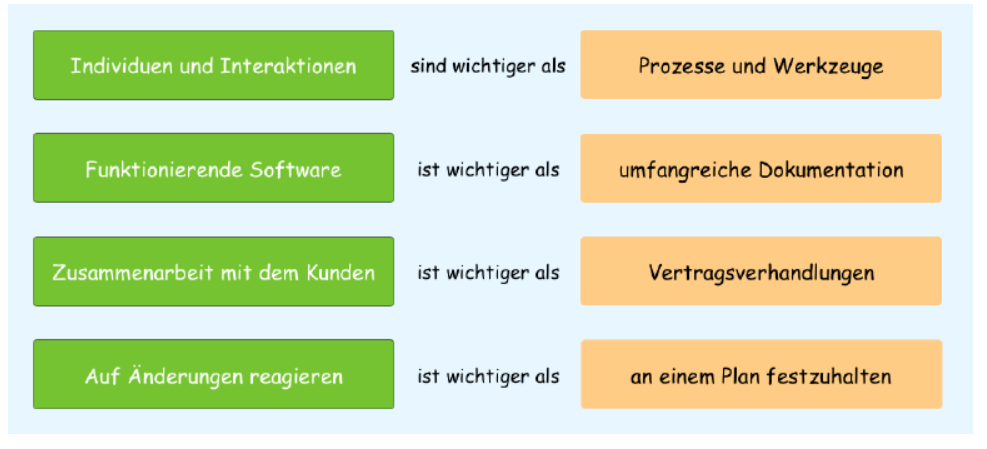
\includegraphics[width=1\textwidth]{figures/daniel/Bild-1.png}
  \caption[]{Scrum Prinzipien verglichen}
  \label{fig:scrum_prinzipien}
\end{figure}

Frei interpretiert wird beim Scrum Framework mehr Wert auf die einzelnen Stakeholder des Projekts gelegt als auf das Projekt selbst. Ebenso werden Bürokratie und umfangreiche Planungen auf ein nötigstes reduziert. Der Ansatz verfolgt dem klaren Ziel, Teilerfolge schnell sichtbar zu machen und den Kunden in frühen Stadien der Arbeit mit in den Projektfortschritt zu integrieren. 

\subsection{Scrum Rollen}
\subsubsection{Product Owner}
Als Product Owner, am ehesten zum klassischen Projektmanagement mit dem Projektleiter vergleichbar, repräsentiert die Bedürfnisse des Endkunden und steht im engen Austausch mit dem Auftraggeber. Seine Aufgabe ist es, die Bedürfnisse des Kunden genau zu verstehen und diese bestmöglich umsetzen zu lassen. Er hat eine klare Vision und vergleicht sprintweise den Fortschritt seines Teams und dem resultierenden Inkrement mit der tatsächlichen Wunschsoftware des Kunden. 

\subsubsection{Scrum Master}
Der Scrum Master, ist in dieser Rolle und Funktion einzigartig im gleichnamigen Framework. Er steht für Teamchemie und Prozessreife, gleichzeitig unterstützt er das Team und den Product Owner und gilt als Problemlöser. Der Zauber in seiner Funktion ist die Eigenständigkeit gegenüber dem eigentlichen Product Owner. Er steht als Mittelsmann in vielerlei Hinsicht. Das Team zu verstehen und die Zusammenarbeit und Kommunikation zu verbessern und fördern ist sein Ziel, nicht der direkte Projekterfolg und die Erfüllung der Kundenbedürfnisse.

\subsubsection{Team}
Das Team ist verglichen mit dem klassischen Projektmanagement eher selbstorganisierter und eigenverantwortlicher in der Erfüllung der vom Projektleiter vorgegebenen Aufgaben. Es wird in regelmäßigen Terminen, später näher erläutert viel über Kommunikation und Austausch koordiniert als stets das stumpfe Erledigen von Aufgaben. Das Einbringen von Ideen und das Kundtun von Problemen und Missständen ist essenziell für den Projekterfolg. 


\subsection{Scrum Artefakte}
\subsubsection{Product Backlog}
Das Product Backlog ist am ehesten mit einem Milestoneplan aus dem klassischen Projektmanagement zu vergleichen. Es stellt eine Liste aller offenen Aufgaben dar und wird vom Product Owner gehegt und gepflegt. Er priorisiert hier sprintweise die zu erledigenden Tätigkeiten nach Wichtigkeit und Dringlichkeit und will für den Kunden den maximal möglichen Umfang rausholen gleichzeitig aber mit enger Abstimmung seines Teams nach deren Möglichkeiten und mit deren technischer Expertise.

\subsubsection{Sprint Backlog}
Der Sprint Backlog ist ein Extrakt aus dem zuvor beschriebenen Product Backlog, reduziert auf die Tätigkeiten eines Sprints. Mit einer Laufzeit von beispielsweise 6 Wochen wird ein gemeinsames Ziel definiert und die dafür zu erfüllenden Aufgaben werden durch den Sprint Backlog als Liste festgehalten. Es erfolgt hier ebenso eine Priorisierung und Zuordnung auf Personen. Die einzelnen Teammitglieder nehmen sich den darin stehenden Aufgaben an und berichtet regelmäßig und eigenständig über den Status der Fertigstellung oder über auftretende Probleme oder benötigte Unterstützung jeglicher Art.

\subsubsection{Product Inkrement}
Das Product Inkrement stellt ein einzelnes Teilergebnis nach einem Sprint dar, auf welches im selbigen hingearbeitet wird. Es soll ein vorzeigbarer und erlebbarer Bestandteil des Gesamtergebnisses sein, welches mit dem Kunden gemeinsam diskutiert wird. Am Produkt Inkrement bekommt das gesamte Team relativ früh und konkret Kundenfeedback über die Zufriedenheit der bisher geleisteten Arbeit. Missverständnisse und Fehler in der Umsetzung sollen sehr schnell aufgezeigt werden.

\subsection{Scrum Events}
\begin{figure}[!htb]
  \centering
  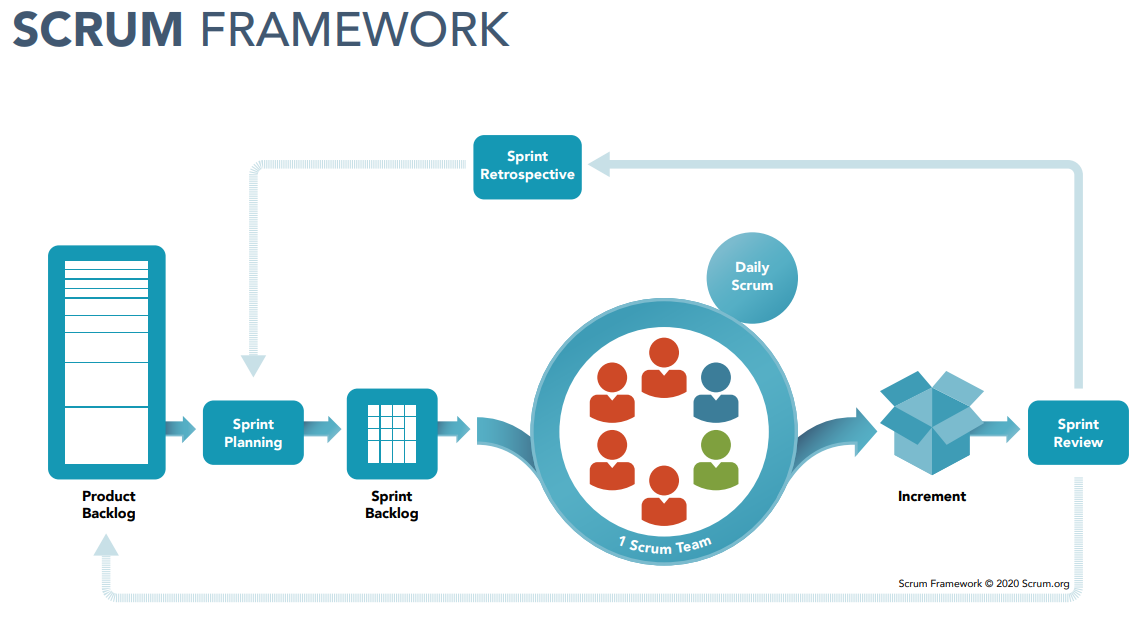
\includegraphics[width=1\textwidth]{figures/daniel/Bild-2.png}
  \caption[]{Scrum-Events im Überblick}
  \label{fig:scrum_events}
\end{figure}

\subsubsection{Sprint}
Der bereits erwähnte Sprint stellt einen Teilabschnitt des Projekts dar. Er besitzt einen eigenen Backlog und wird in der Regel auf 4-8 Wochen terminiert. Innerhalb des Sprints bestimmen weitere Events den Rahmen des Frameworks. Der Sprint selbst steht repräsentativ für das agile Projektmanagement und unterscheidet dich somit klar vom klassischen, oft im Wasserfall ausgelebten Projektmanagement, welches oft nur als Ganzes gesehen wird mit festen Milestones als Einzeletappen.

\subsubsection{Sprint Planning}
Das Sprint Planning stellt den Beginn eines neuen Sprints dar. Hier wird ein Product Inkrement festgelegt, ein gemeinsames Ziel formuliert und deren dafür benötigten Aufgaben definiert. Das Team als Ganzes ist in der Planung involviert. Die Planung selbst erfolgt oftmals über das sogenannte Planning Poker, jedoch kann dieses auch anders praktiziert werden. Jedes einzelne Teammitglied sollte im Austausch mit dem Team selbst und dem Produktowner sowie Scrum Master seinen Arbeitsumfang im Sprint festlegen.



\subsubsection{Weekly Standup}
Das Weekly Standup oftmals auch als Daily Standup praktizierte Event, stellt einen Regeltermin für das gesamte Team dar, in welchem die einzelnen Teammitglieder Ihren aktuellen Arbeitsfortschritt kundtun beziehungsweise kommende Aufgaben und Herausforderungen mit dem Team teilen. Es sollte als kurzes und agiles Event praktiziert werden in welchem auf Probleme und Schwierigkeiten offen und ehrlich mitgeteilt werden. Bei physisch gehaltenen Termin werden die Mitglieder des Termins oft stehend in den Austausch gebracht, online kann dieses zumindest jeder selbst frei entscheiden.

\subsubsection{Sprint Review}
Im Review wird der nun abgeschlossene Sprint begutachtet und der Fortschritt und der Erfolg und Misserfolg objektiv beurteilt. Jedes Mitglied kann seine Aufgaben und Ergebnisse individuell oder als Teil-Team vorstellen und diese gegenüber dem Kunden beziehungsweise dem restlichen Team präsentieren. Es ist darauf zu achten das Event selbst klar von der kommenden Retroperspektive abzugrenzen und persönliche Themen für dieses Event aufzuheben. Der Kunde selbst ist in diesem Event oft involviert.


\subsubsection{Sprint Retrospective}
Die Sprint Retrospective oder auch als Retro bezeichneter Termin, findet gegen Ende des vorangegangenen Sprints statt. Im Gegensatz zum zuvor erwähnten Review werden hier subjektive und zwischenmenschliche Themen miteinander diskutiert. Das Event soll die Möglichkeit schaffen, sich als Team auszutauschen und gegenseitig mit Lob und konstruktiver Kritik zu konfrontieren. Hier ist vor allem der Scrum Master gefragt, eine Atmosphäre zu schaffen und das Team zu ermutigen oft auch unangenehme Themen anzusprechen.

\section{Projektmanagement}
\label{sec:projectmanagement}
% \section{Projectmanagement}

In diesem Abschnitt wird der Bereich des Projektmanagements und der Projektplanung innerhalb des Digital Home Town Teams näher erläutert. Als Hilfsmittel wurde hierfür hauptsächlich die Software JIRA von Atlassian verwendet. Hierbei wird auch auf die einzelnen Tasktypen und deren Bedeutung eingegangen. Des Weiteren wurde ein eigener Arbeitsablauf für das Entwicklerteam definiert. Abschließend wird auf die Sprint-Planung und die spätere Verwendung einer sog. User Story Map eingegangen.

\subsection{JIRA}
JIRA ist ein Tool zur Unterstützung von Projektmanagement-Prozessen, das von vielen Unternehmen und Organisationen genutzt wird. Mit JIRA können Projekte geplant, verwaltet und kontrolliert werden, indem Aufgaben, Meilensteine und Prozesse visualisiert und koordiniert werden. Es bietet auch Funktionen zur Zusammenarbeit und Kommunikation innerhalb des Projektteams sowie zur Nachverfolgung von Fortschritten und Problemen. JIRA kann auch individuell angepasst werden, um den spezifischen Bedürfnissen eines Projekts gerecht zu werden. Im Zuge des Projekts wurden mehrere solcher Anpassungen vorgenommen sowie Teaminterne Regeln festgelegt. Diese sollen im Folgenden Abschnitt näher erläutert werden.

\subsubsection{Tasks}
Die Besonderheit an JIRA ist die Möglichkeit zur Aufteilung von mehreren Arbeiten in sogenannte Tasks. Ein Task hat normalerweise eine eindeutige Identifikationsnummer, eine kurze Beschreibung der Aufgabe, eine Zuweisung an einen Verantwortlichen, einen Status sowie ggf. zusätzliche Informationen wie z.B. Verknüpfungen mit anderen Tasks. 

\begin{figure}[ht!]
    \centering
    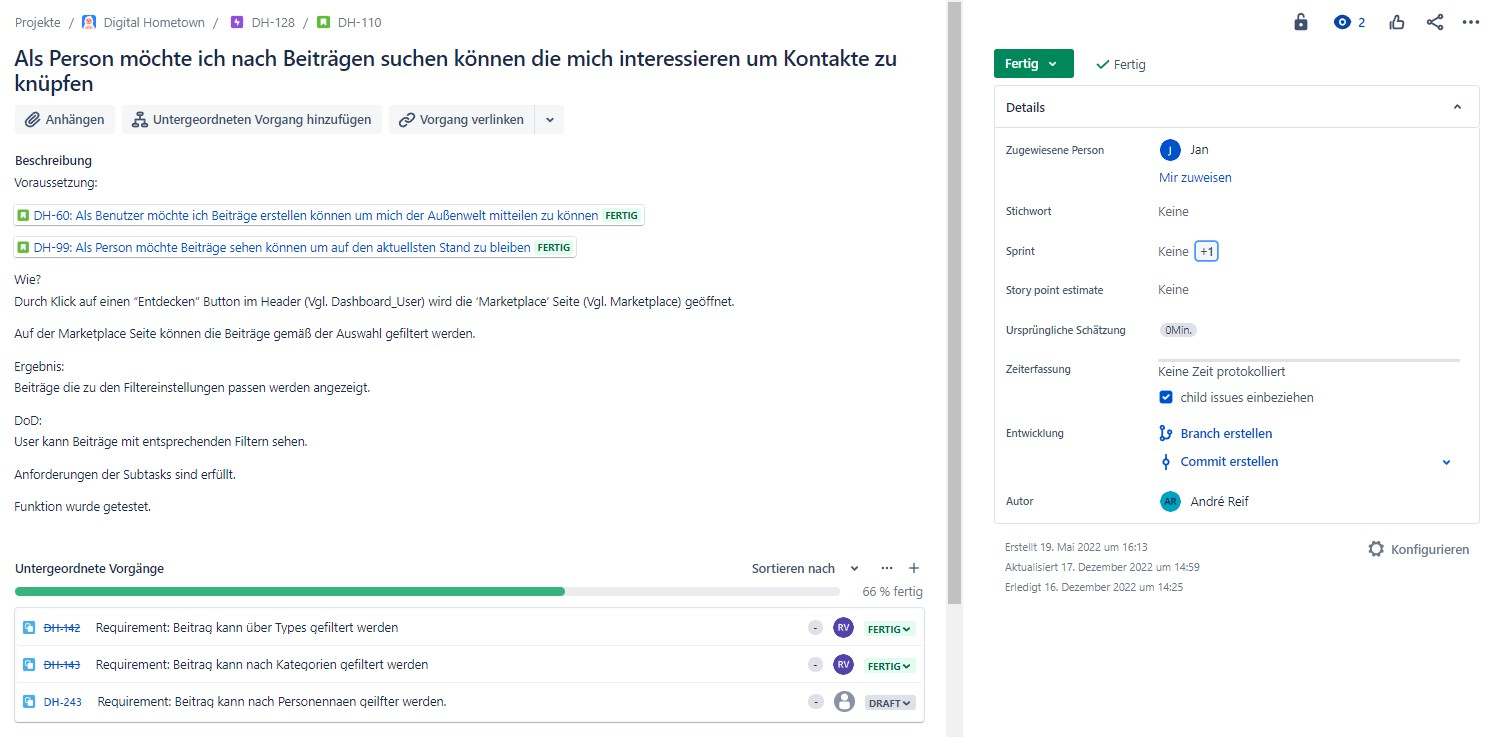
\includegraphics[width=0.6\textwidth]{figures/andre/jiratask.jpg}
    \caption{Beispiel für einen Task im JIRA}
    \label{fig:jiratask}
\end{figure}

Einzelne Tasks können in sog. Epics geclustert werden, um so die Aufgaben und langfristige Planung besser strukturieren zu können. Im Folgenden ist eine Übersicht der Epics innerhalb des Projekts sowie deren Fortschritt zu sehen.

\begin{figure}[ht!]
    \centering
    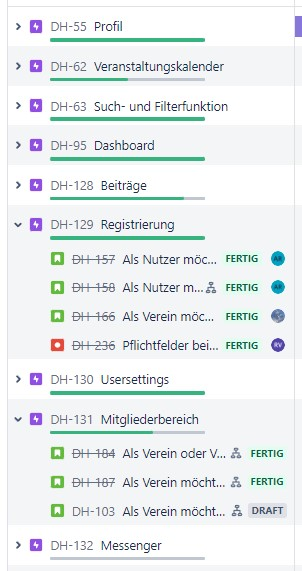
\includegraphics[width=0.6\textwidth]{figures/andre/epicsdesprojekts.jpg}
    \caption{Epic Übersicht des Projekts}
    \label{fig:epicsdesprojekts}
\end{figure}

Für die einzelnen Tasks wurden jeweils 4 verschiedene Typen unterschieden.

\subsubsection*{User-Story}
Eine User Story beschreibt eine neue Nutzeranforderung, also ein Feature, dass umgesetzt werden muss das der Benutzer die entsprechende Tätigkeit ausführen kann. Diese werden per Definition nach dem folgenden Prinzip geschrieben:

Als Nutzer möchte ich \textbf{<Auszuführende Tätigkeit>} um \textbf{<Vorteil oder Intention der ausgeführten Tätigkeit>}.

Eine User Story hat den Folgenden Aufbau:
\begin{itemize}
    \item \textbf{Titel} User Story nach Definition.
    \item \textbf{Wie?} Kurze Beschreibung wie die Funktion umgesetzt werden soll.
    \item \textbf{Ergebnis?} Beschreibung was passiert, wenn die Funktion ausgeführt wird.
    \item \textbf{DoD} Definition of Done, also eine Definition, wann der Task als erledigt gilt.
\end{itemize}

\subsubsection*{Sub-Task}
Sub-Tasks werden in der Regel dazu verwendet, um besonders aufwendige User Stories und Tasks in kleinere Arbeitseinheiten zu unterteilen. Für Digital Home Town wurden die Sub-Tasks verwendet, um Task-spezifische Anforderungen zu dokumentieren und hervorzuheben. 
\subsubsection*{Functional-Task}
Für unterstützende Arbeiten, die nicht direkt mit der Entwicklung der Plattform in Verbindung stehen, wurden sog. Functional Tasks eingeführt. Diese sind in der Regel nicht näher definiert oder Beschrieben und sind Anhand des Titels nachvollziehbar. 

\begin{figure}[ht!]
    \centering
    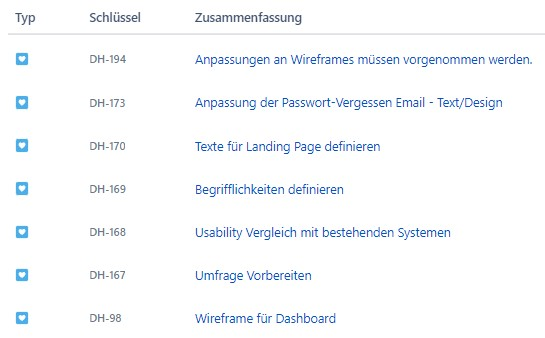
\includegraphics[width=0.6\textwidth]{figures/andre/functionaltasks.jpg}
    \caption{Beispiele für Functional Tasks}
    \label{fig:functionaltasks}
\end{figure}

\subsubsection*{Bug}
Ein Bug stellt einen gefundenen Fehler auf der Plattform da. Dieser spiegelt sowohl einen Fehlerbericht als auch einen neuen Arbeitsauftrag dar. Innerhalb des Entwicklerteams war es üblich, dass zumeist der Verursacher des Bugs auch für dessen Behebung verantwortlich war. Ein Bug durchläuft allerdings denselben Arbeitsablauf wie eine User-Story und nach den gleichen Standards getestet.

\begin{figure}[ht!]
    \centering
    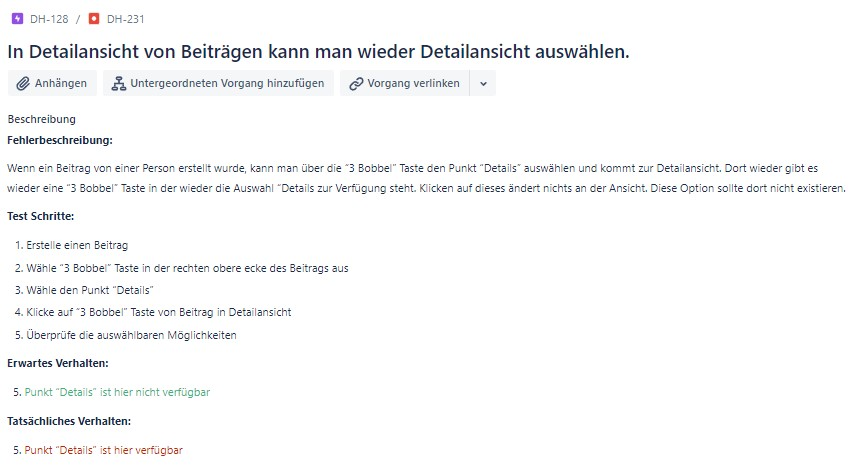
\includegraphics[width=0.6\textwidth]{figures/andre/bugticket.jpg}
    \caption{Beispiel für ein Bug Ticket}
    \label{fig:bugticket}
\end{figure}

Ein Bug besteht in der Regel aus:

\begin{itemize}
    \item \textbf{Titel} Kurze Beschreibung des Fehlers
    \item \textbf{Beschreibung} Detaillierte Beschreibung des Fehlers und des Fehlerhergangs
    \item \textbf{Test Schritte} Schritt-für-Schritt Angaben über den Ablauf des Tests
    \item \textbf{Verhalten} Erwartetes und Tatsächliches Verhalten
\end{itemize}

\subsubsection{Arbeitsablauf}
In der folgenden Abbildung ist der Allgemeine Arbeitsablauf für ein einzelnes JIRA Ticket zu sehen.

\begin{figure}[h!]
    \centering
    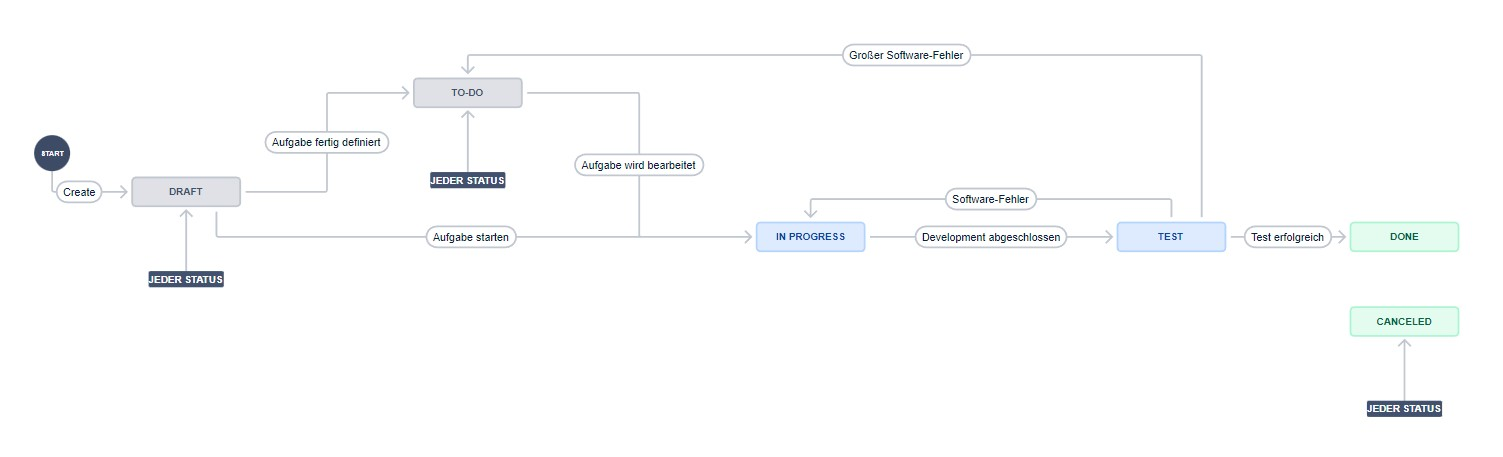
\includegraphics[width=0.6\textwidth]{figures/andre/workflow.jpg}
    \caption{Darstellung des Ablaufs eines einzelnen JIRA Tickets}
    \label{fig:workflow}
\end{figure}

Ein einzelner Task wurde zunächst mit dem Status „Draft“ erstellt. Dies wurde im Allgemeinen so interpretiert, dass das Ticket zwar angelegt wurde, jedoch nicht vom Team so akzeptiert wurde, dass jeder die Aufgabe verstanden hat. Dies wurde bei der Sprint Planung bzw. dem Task Refinement während der Planung Besprochen, ggf. angepasst, und dann festgelegt. 

Nachdem ein Task den Status „ToDo“ erhält, kann dieser in einem Sprint eingeplant und entsprechend bearbeitet werden. Der Status wechselt demnach zu „In Progress“. 

Nach der Bearbeitung wird ein Ticket mit Hilfe des Flags „Test“ zum Testen freigegeben. Das Bedeutet der Code läuft in der Entwicklungsumgebung und kann von einem Tester bearbeitet werden. Ob im Fehlerfall ein Task zurück in den Status „ToDo“ oder „In Progress“ versetzt wurde, lag in der Schwere des Fehlers und im Ermessen des jeweiligen Testers. Falls der Test erfolgreich war, wurde der Task auf den Status „Done“ verschoben und war somit abgearbeitet.

Aufgrund sich ändernder Anforderungen wurde später der „Canceled“ Staus eingeführt, um ggf. bereits begonnene Tasks abbrechen zu können.

Dieser Ablauf gilt in der Regel für jede User Story sowie jeden Bug. Die Stati „Draft“ und „Test“ hatten für Functional Tasks und Sub Tasks jedoch keine tiefergehende Bedeutung und konnten einfach übersprungen werden.

\subsection{Sprint Planning mit JIRA}
Die Sprints wurden in der Regel vorausgeplant. Dabei galt die Regel: der nächste Sprint steht am Ende des aktuellsten Sprints weitestgehend fest, der übernächste Sprint ist zu 50\% geplant. 

Während der Planungsmeetings wurden die geplanten Tasks und Bugs besprochen und auf deren Umsetzbarkeit und Priorität geprüft. Aufgrund der un-terschiedlichen Kenntnisse und Fertigkeiten der Entwickler war es jedoch schwierig den Aufwand einzelner Tasks verallgemeinert für das gesamte Entwicklungsteam einzuschätzen. Zuzüglich dazu mussten Urlaubs- und Abwesenheitszeiten bei der Planung berücksichtigt werden, sodass die definierten Sprint Ziele auch erreicht werden konnten.

\begin{figure}[h!]
    \centering
    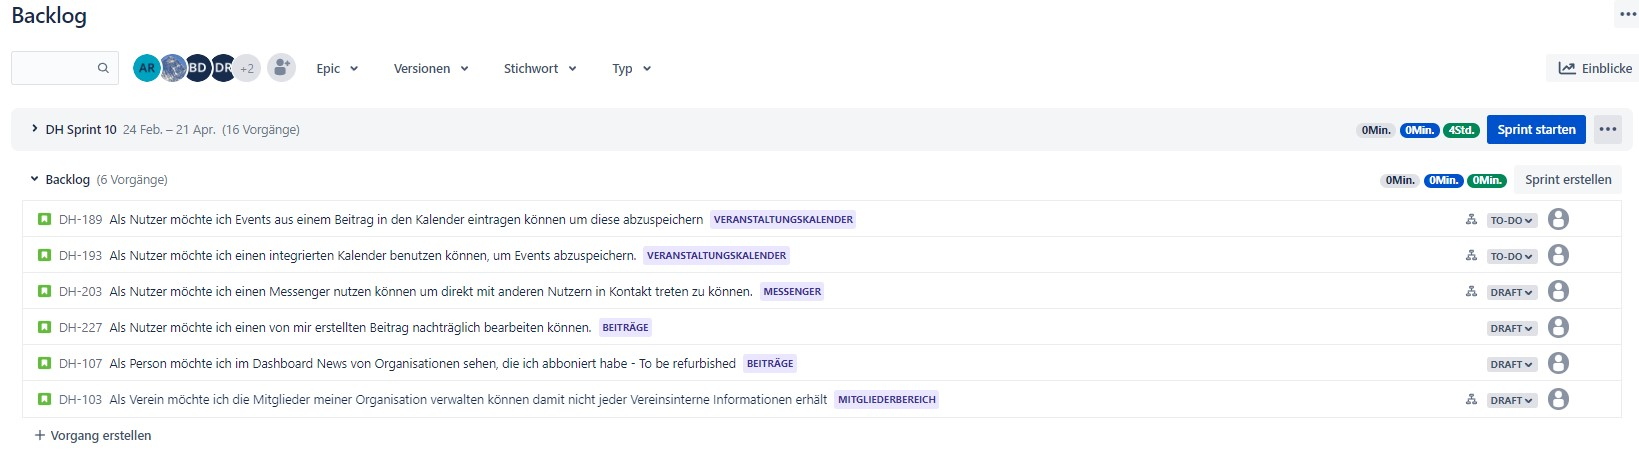
\includegraphics[width=0.6\textwidth]{figures/andre/jirabacklog.jpg}
    \caption{Backlog Funktion im JIRA}
    \label{fig:jirabacklog}
\end{figure}

Zur Planung der Sprints wurde die in der obigen Abbildung zu sehende Backlog Funktion verwendet. Hier sind zum sowohl die nicht geplanten Tasks zu sehen als auch die einem Sprint bereits zugeordnetem Task und können auch bei Bedarf entsprechend umgeplant werden. So war es nicht unüblich, dass nachdem das Sprintziel bereits vor dem Ende des Sprints erreicht wurde, noch offene Bugs oder kleinere Functional Tasks dem Sprint hinzugefügt und abgearbeitet wurden. Zum Sprintende begonnene Arbeitsaufträge wurden grundsätzlich in den nachfolgenden Sprint verschoben und fertiggestellt.

\subsubsection{User Story Map}
Als weiteres Tool zur Projektplanung wurde der Ansatz des sogenannten User Story Mapping verwendet. Per Definition ist eine User Story Map eine Technik zur Visualisierung von Benutzeranforderungen und -funktionen in einer hierarchischen Struktur.

\begin{figure}[h!]
    \centering
    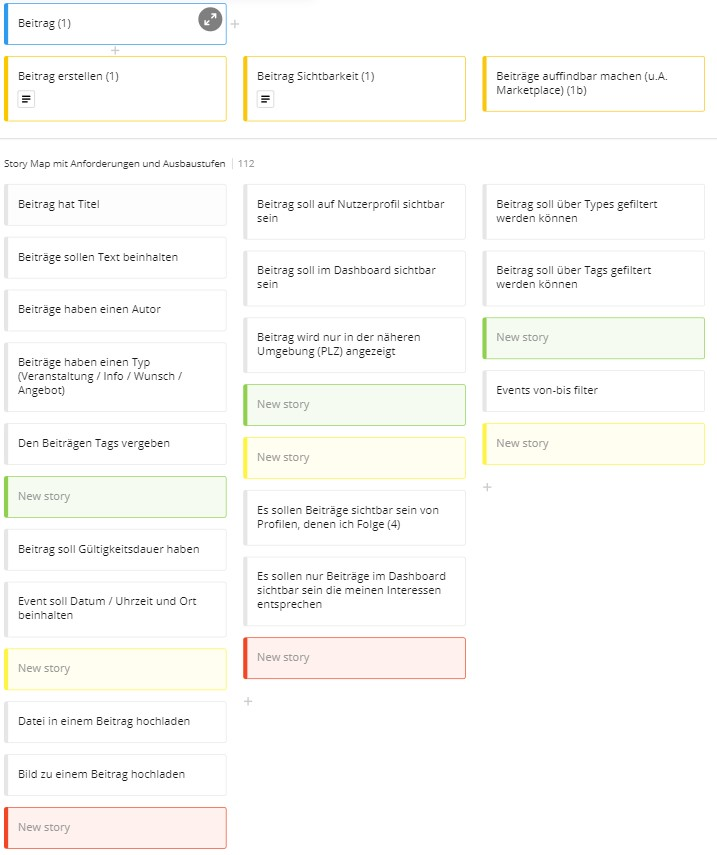
\includegraphics[width=0.6\textwidth]{figures/andre/userstorymap.jpg}
    \caption{Beiträge in der User Story Map}
    \label{fig:userstorymap}
\end{figure}

In der obigen Abbildung ist die User Story Map für einige Features der Beiträge zu finden. So gibt es zur User Story „Als Nutzer möchte ich einen Beitrag erstellen können um mich der Community mitteilen zu können“ verschiedene Anforderungen. Diese stehen unterhalb des jeweils gelben Blocks. 

Die Anforderungen jeweils wurden dann in 3 Iterationsstufen Priorisiert:

\begin{itemize}
    \item \textbf{Bis Grün} Minimum viable product, also die Minimalanforderungen die Umgesetzt werden sollen
    \item \textbf{Bis Gelb} Nice-to-Have, Anforderungen die umgesetzt werden sollen, aber nicht hoch Priorisiert werden
    \item \textbf{Bis Rot} Wird implementiert falls genügend Zeit dafür da ist
\end{itemize}

Aus dieser Map wurden dann die einzelnen User Story Tasks im JIRA angelegt und entsprechend in den Sprints verplant.

\section{Sprintübersicht}
\label{sec:sprintoverview}
\input{content/03_process/03_Sprintübersicht}

\chapter{Analyse}
\label{ch:analysis}

\section{Wettbewerbsanalyse}
\label{sec:competitionanalysis}
\label{sec:Wettbewerbsanalyse}

Um die Bedürfnisse zukünftiger Nutzer zu erfüllen und das Produkt langfristig wettbewerbsfähig zu halten, ist es unerlässlich, kontinuierlich alle relevanten Kundenanforderungen zu ermitteln und zu priorisieren. Zusätzlich ist es wichtig, sich mit Wettbewerbern, ihren Produkten und Strategien auseinanderzusetzen, um die eigenen Marktchancen zu bewerten. Eine Analyse gibt zudem Aufschluss darüber, welche Features bereits als grundlegend erwartet werden und welche Möglichkeiten es gibt, um sich von anderen Anbietern zu differenzieren.


Die Wettbewerbsanalyse wurde in mehreren Schritten durchgeführt:

\begin{itemize}
    \item Ermittlung der Hauptwettbewerber
    \item Erstellung eines Konkurrenzprofils
    \item Darstellung der einzelnen Wettbewerber
    \item Bewertung der strategischen Ausrichtung
    \item Zusammenfassung der Ergebnisse
\end{itemize}

\subsection{Ermittlung der Hauptwettbewerber}

Für die Identifikation der bedeutendsten Mitbewerber ist es wichtig, die Hauptmerkmale und Ziele des eigenen Dienstes zu kennen und mit potenziellen Wettbewerbern abzugleichen. Dabei sollte berücksichtigt werden, dass es in der digitalen Welt nicht immer Wettbewerber gibt, die exakt den gleichen Dienst anbieten oder dieselbe Strategie verfolgen. Dennoch können mittelfristig vollwertige Konkurrenzprodukte entstehen, die zum Zeitpunkt der Analyse nur wenige gemeinsame Parallelen oder Features aufweisen.

Die langfristige Ausrichtung von \acrfull{dht} besteht darin, den lokalen/regionalen Raum und seine sozialen Verflechtungen zu stärken, indem der digitale Austausch zwischen allen Personen und Institutionen gefördert wird, die das örtliche Dasein widerspiegeln. Die Schwerpunkte von \acrshort{dht} sind wie folgt:

\begin{enumerate}
    \item Das Vernetzen von Personen, die gleiche Interessen oder ähnliche Bedürfnisse haben und einen Austausch von Informationen, Waren und Dienstleistungen anstreben oder Unterstützung und Hilfestellung suchen bzw. anbieten.
    \item Die Stärkung lokaler Vereine und Dienstleistungen, damit diese ihre Angebote gezielter darstellen und leichter mit Interessenten in Kontakt treten können.
    \item Die Unterstützung öffentlicher Einrichtungen, um einen einfacheren Zugang zu amtlichen Informationen, Terminen und anderen Ressourcen zu ermöglichen.
\end{enumerate}

Zugleich verpflichtet sich \acrshort{dht} dazu, allen Nutzern einen barrierefreien Zugang zu ermöglichen.

Basierend auf den Zielen von \acrshort{dht} wurden verschiedene Webdienste identifiziert, die sich auf den lokalen Raum und den Austausch, die Vernetzung oder die Zusammenführung von Privatpersonen konzentrieren. Zunächst wurden als etablierte und aktive Vertreter in mindestens einem der genannten Bereiche identifiziert:

\begin{itemize}
    \item Facebook,
    \item Nebenan.de,
    \item Spontacts,
    \item eBay Kleinanzeigen und
    \item Doctolib.
\end{itemize}

Im Folgenden werden beispielhaft nur die Vertreter aus dem Bereich Social Networking näher betrachtet, zu denen Facebook, Nebenan.de und Spontacts zählen.

\subsection{Konkurrenzprofil}

Für eine eingehende Analyse der ermittelten Wettbewerber ist es notwendig, individuelle Konkurrenzprofile für jeden Marktteilnehmer zu erstellen. Diese Gegenüberstellung des eigenen Selbstprofils bietet eine transparente Bewertungsbasis, die wertvolle Erkenntnisse über Stärken, Potenziale und strategische Ziele liefert.

Folgende Punkte werden bei der Konkurrenzanalyse gesondert betrachtet:

\begin{itemize}
    \item Fokus des Dienstes und Zielgruppe
    \item Möglichkeiten der Selbstdarstellung und des Austauschs
    \item Benachrichtigungen über Änderungen und Neuigkeiten
    \item Entdecken von Inhalten
\end{itemize}

\subsection{Kurzdarstellung}

\subsubsection{Facebook}

\acrfull{fb} ist ein weltweit bekannter und etablierter Dienst, der es Nutzern ermöglicht, sich mit Menschen aus aller Welt zu vernetzen, in Kontakt zu bleiben und Inhalte aus ihrem Leben mit anderen zu teilen.
Ursprünglich richtete sich der Fokus von \acrshort{fb}  auf Studenten, aber im Laufe der Jahre hat sich die Zielgruppe verbreitert und ist heute sehr heterogen.

\begin{figure}[!htb]
    \centering
    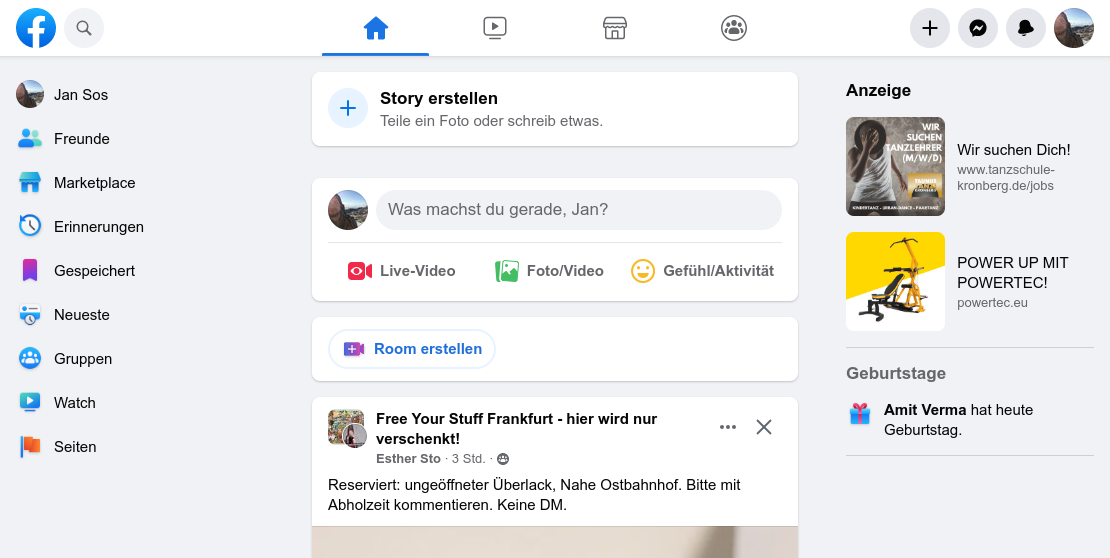
\includegraphics[width=\textwidth]{figures/jan/pic_facebook.png}
    \caption[Startseite von \acrshort{fb}]{Startseite von Startseite von \acrshort{fb}}
    \label{fig:facebook}
\end{figure}

Die Nutzung von \acrshort{fb} ist sehr vielfältig und hängt von den Bedürfnissen des einzelnen Nutzers ab. Neben reinen Darstellungs- und Austauschmöglichkeiten bietet \acrshort{fb} eine breite Palette von Anwendungen an, wie z.B. integrierte Video-, Game- und Datingportale sowie ein eigenes Bezahlsystem. Auf diese speziellen Anwendungen wird im weiteren Verlauf nicht weiter eingegangen.

\paragraph{Selbstdarstellung}

Für die Selbstdarstellung von Organisationen oder Personen bietet \acrshort{fb} ein eigenes Profil an, auf dem Bilder, persönliche Informationen und Vorlieben wie Musik öffentlich dargestellt werden können. Die Sichtbarkeit dieser Inhalte kann individuell angepasst werden. Neben den statischen Informationen enthält das Profil auch eine Pinnwand, auf der ältere und aktuelle Beiträge listenmäßig aufgeführt werden.

\paragraph{Formen des Austausches}

Beiträge ermöglichen den interaktiven Austausch und das Teilen von Momenten. Jeder Nutzer kann sie verfassen und auf seiner eigenen sowie auf fremden Pinnwänden veröffentlichen. Ereignisse wie das Hochladen von neuen Bildern generieren automatisch einen Beitrag, um Bekannte, Follower und andere Personen über Neuigkeiten im Profil zu informieren. Beiträge lassen sich neben einfachem Text auch mit Bildern oder Videos sowie mit Tags (Orte, GPS, Veranstaltungen, Personen, etc.) spezifizieren. Andere Nutzer können Beiträge kommentieren oder bewerten.

\acrshort{fb}-Gruppen ermöglichen den Austausch mit mehreren Personen zu gemeinsamen Themen. Ähnlich wie Profile haben Gruppen einen statischen Teil, in dem Administratoren eine Kurzbeschreibung der Gruppe veröffentlichen. Eine Pinnwand ermöglicht den Mitgliedern die Kommunikation untereinander. Durch das Erstellen von Events können Gruppenmitglieder gemeinsame Treffen oder Aktivitäten planen.\\
Gruppen werden sehr häufig und für verschiedene Themen genutzt. Insbesondere im städtischen Raum dienen sie zum Beispiel dem Verschenken von ungenutzten Dingen, dem Knüpfen neuer Kontakte in einer neuen Stadt oder dem Treffen von Menschen in der Nähe mit ähnlichen Hobbies. Auch der Austausch über diverse Themen in unterschiedlichen Bereichen auf regionaler, nationaler und internationaler Ebene ist weit verbreitet.

Der Austausch materieller Gegenstände findet hauptsächlich auf einem digitalen Marktplatz statt. Die geschalteten Anzeigen enthalten eine Überschrift, eine freie Beschreibung, Bilder, Angaben zum Zustand, zur Preisvorstellung, zum Ort und zum Herausgeber der Anzeige. Der Verfasser muss bei der Erstellung der Anzeige eine vordefinierte Kategorie auswählen, um die Auffindbarkeit zu erleichtern. Neben der direkten Kontaktaufnahme besteht für Interessenten die Möglichkeit, die Anzeige zu merken, mit einem Kontakt zu teilen oder einen Alarm zu erstellen, sobald ähnliche Produkte angeboten werden.

Auf \acrshort{fb} können Kontakte gepflegt werden, indem man sich gegenseitig in eine Freundesliste aufnimmt. Über diese Liste können Inhalte selektiv verteilt werden, so dass sie nur für \textit{Freunde} sichtbar sind. Zusätzlich werden \textit{Freunde} über das Dashboard gezielt informiert, wenn ein \textit{Freund} einen neuen Beitrag erstellt hat.

Für den direkten und privaten Austausch bietet \acrshort{fb} einen Chat an, in dem sowohl 1:1- als auch Gruppenchats möglich sind. Die Kommunikation erfolgt in Echtzeit und die Nachrichten können wie Beiträge Bilder, Links und andere Inhalte enthalten. In 1:1-Gesprächen besteht auch die Möglichkeit, Sprach- und Videoanrufe zu tätigen.

\paragraph{Neuigkeiten}

Um bei der Vielzahl der Beiträge und Reaktionen von Freunden oder Gruppen den Überblick zu behalten, bietet \acrshort{fb} ein Dashboard an, auf dem Neuigkeiten in Form einer endlosen und unsortierten Liste angezeigt werden. Das Dashboard enthält auch kommerzielle Werbung und Beiträge von Gruppen, die der Nutzer noch nicht abonniert hat, aber von Interesse sein könnten.

Neben dem Dashboard gibt es auch eine Notifications-Seite, die einen gezielteren Fokus auf das Wesentliche ermöglicht. Hier werden kurze Benachrichtigungen wie Geburtstage von \textit{Freunden}, bevorstehende Events, neue Beiträge aus abonnierten Gruppen sowie Reaktionen auf eigene oder kommentierte Beiträge angezeigt.

\paragraph{Recherche}

\acrshort{fb} bietet eine Suchfunktion, die es Nutzern ermöglicht, nach Personen, Gruppen und anderen Inhalten zu suchen. Die Suchergebnisse können durch verschiedene Filter wie Art des Inhalts, Verfasser, Gruppen, Zeitraum und mehr genauer spezifiziert werden.

Zusätzlich können Nutzer Beiträge und öffentliche Profile als \textit{Bookmarks} sichern. Die \textit{Bookmarks} können dann auf einer dafür vorgesehenen Seite je nach Typ aufgelistet und verwaltet werden.

\subsubsection{Nebenan.de}

Nebenan.de ist eine Plattform, die im Jahr 2015 gestartet wurde und wie \acrshort{fb} darauf abzielt, Menschen zu vernetzen (Abb. \ref{fig:nebenan}). Der Unterschied zu \acrshort{fb} besteht darin, dass sich Nebenan.de ausschließlich auf die unmittelbare Nachbarschaft des Nutzers konzentriert.

\begin{figure}[!htb]
    \centering
    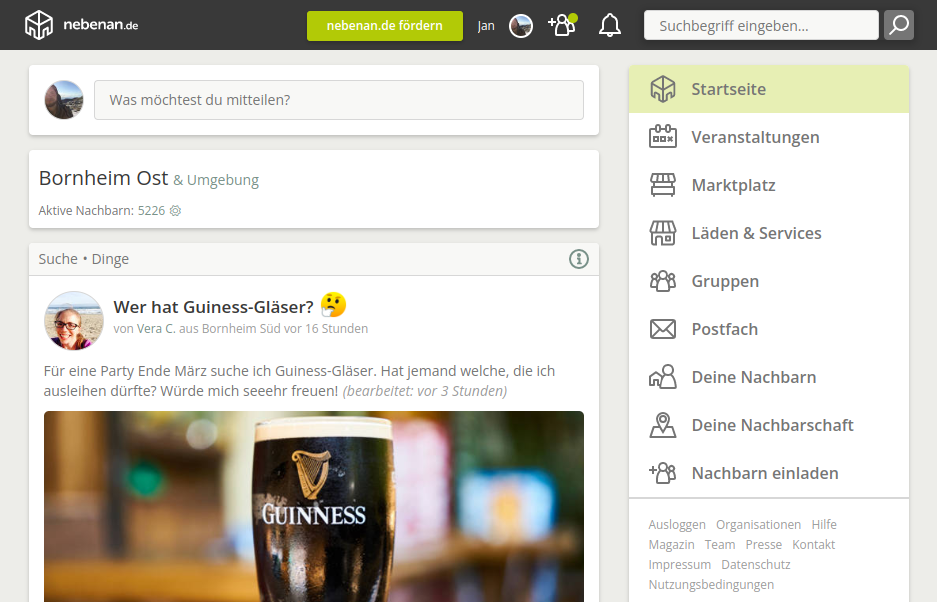
\includegraphics[width=\textwidth]{figures/jan/pic_nebenan.png}
    \caption[Startseite von nebenan.de]{Startseite von nebenan.de}
    \label{fig:nebenan}
\end{figure}

Die Zielgruppe umfasst alle Interessengruppen, die in der Nachbarschaft des Benutzers vertreten sind, wie z.B. Anwohner, Vereine, Firmen und Organisationen. Die Nachbarschaftsgrenze wird vom System anhand der eigenen Adresse des Nutzers definiert und kann nicht individuell angepasst werden.

\paragraph{Selbstdarstellung}

Für die Darstellung existieren auf Nebenan.de zwei Arten von Profilen. Die erste Profilart gilt für Einzelnutzer. Hierbei können sich Anwohner über ein Kurzprofil mit Foto, einem Freitext sowie ihren Interessen und Angeboten vorstellen. Zur Auswahl der Interessen und Angebote gibt es fest definierte Vorschläge, um zu beschreiben, was der Anwohner in die Nachbarschaft einbringen kann. Dazu zählen beispielsweise das \textit{Annehmen von Paketen}, das \textit{Blumengießen}, die \textit{Reparatur von Fahrrädern} oder das \textit{Gesellschaft leisten}. Das Profil zeigt auch die Aktivitäten des Anwohners an, wie beispielsweise beigetretene nebenan-Gruppen und die Anzahl der erhaltenen virtuellen Dankeschöns. \\
Organisationen und Läden/Services, die vor Ort angesiedelt sind und zum alltäglichen Leben in der Nachbarschaft beitragen, nutzen die zweite Profilart. Diese Profile enthalten im Vergleich zu den Anwohnerprofilen deutlich mehr Informationen und müssen beim Anlegen einer Kategorie zugeordnet werden, wie z.B. \textit{Restaurant}, \textit{Reisen}, \textit{Sport}, \textit{Political Party} oder \textit{Nachbarschaftsinitiative}. Neben grundlegenden Informationen wie Name, Adresse, Kontaktdaten und Öffnungszeiten können auch zukünftige Veranstaltungen, Gesuche, Bekanntmachungen, das Verkaufsangebot und weitere Informationen hinterlegt werden. Anwohner können auf den öffentlichen Profilen ihre eigenen Erfahrungen mit der Organisation oder dem Laden teilen und Empfehlungen aussprechen.

\paragraph{Formen des Austausches}

Nebenan.de nutzt den Beitrag als zentrales Mittel für den Austausch zwischen Anwohnern. Jeder Beitrag kann von allen Anwohnern kommentiert und positiv bewertet werden. Beiträge werden bei der Erstellung einer Kategorie zugeordnet, um zu kennzeichnen, ob es sich um ein \textit{allgemeines Thema}, ein \textit{Gesuch}, ein \textit{Angebot}, eine \textit{Empfehlung} oder eine \textit{Veranstaltung} handelt. Jede Kategorie wird in mehrere aufeinander aufbauende Unterkategorien unterteilt, um die Beiträge besser einordnen zu können. \\
Abhängig von der Art des Beitrags werden diese entweder auf dem öffentlichen Dashboard, dem Event-Feed oder dem Marktplatz angezeigt. Ein Beitrag besteht aus einem Titel, einem Freitext und optionalen Bildern. Bei Veranstaltungen können weitere Felder wie Datum und Ort hinzugefügt werden \\
Die Beiträge auf dem Marktplatz werden neben der Hauptkategorie \textit{Angebot} noch weiter in die Unterkategorien wie \textit{Hilfe}, \textit{Schenken}, \textit{Verleihen} oder \textit{Tauschen} unterteilt. Verkaufsangebote können zudem weiter spezifiziert werden, indem sie einer Angebotskategorie wie \textit{Essen}, \textit{Baby \& Kinder} oder \textit{Haustiere} zugeordnet werden. Alle Angebote sind in einer Liste verfügbar und können nach Kategorie gefiltert oder mithilfe der globalen Suchfunktion durchsucht werden.

Um den Austausch unter Menschen mit gemeinsamen Interessen zu erleichtern, bietet nebenan.de die Möglichkeit, Gruppen zu erstellen. Dabei kann der Zweck der Gruppe durch einen aussagekräftigen Namen und eine Beschreibung genauer erläutert werden. In diesen Gruppen können Mitglieder verschiedene Arten von Beiträgen wie Mitteilungen, Suchanfragen, Angeboten oder Veranstaltungshinweisen veröffentlichen. Diese Beiträge erscheinen auf der Gruppenpinnwand und können von allen Gruppenmitgliedern kommentiert werden.

Neben der Gruppenfunktion gibt es auch eine Chatfunktion für den direkten Austausch mit einzelnen Nutzern. Mit dieser Funktion können Nutzer neben reinem Text und Emojis auch Fotos und Empfehlungen verschicken.

\paragraph{Neuigkeiten}

Für die Anzeige von neuen Beiträge steht ein Nachbarschafts-Dashboard zur Verfügung. Hier werden alle Arten von Beiträgen nach dem Datum der letzten Änderung sortiert angezeigt. Der Austausch mit der Nachbarschaft findet hauptsächlich über das Dashboard statt, wo neue Beiträge entdeckt und beantwortet werden können. \\
Zusätzlich werden alle Beiträge, an denen man aktiv teilgenommen hat und bei denen neue Ereignisse aufgetreten sind, nochmals separat in einem Benachrichtungs-Feed aufgelistet, um einen besseren Überblick zu gewährleisten. Darüber hinaus werden im Benachrichtigungs-Feed alle zukünftigen Veranstaltungen in der Nachbarschaft angezeigt.

\paragraph{Recherche}

Die nebenan-Suche bietet eine Möglichkeit zur Suche von Beiträgen jeglicher Art. Interessante Beiträge oder solche, die wichtige Informationen für den Benutzer enthalten, können als Lesezeichen gespeichert werden. Diese Lesezeichen können je nach Art des Beitrages unter \textit{Feed} oder \textit{Marktplatz} eingesehen und bei Bedarf gelöscht werden.

\subsubsection{Spontacts}

Spontacts konzentriert sich im Gegensatz zu \acrshort{fb} und Nebenan.de ausschließlich auf die Organisation von Freizeitaktivitäten für Menschen in der gleichen Region (vgl. Abb. \ref{fig:spontacts}). Die Plattform richtet sich insbesondere an Personen, die Gleichgesinnte für bestimmte Aktivitäten suchen und dabei neue Kontakte knüpfen möchten.

\begin{figure}[!htb]
    \centering
    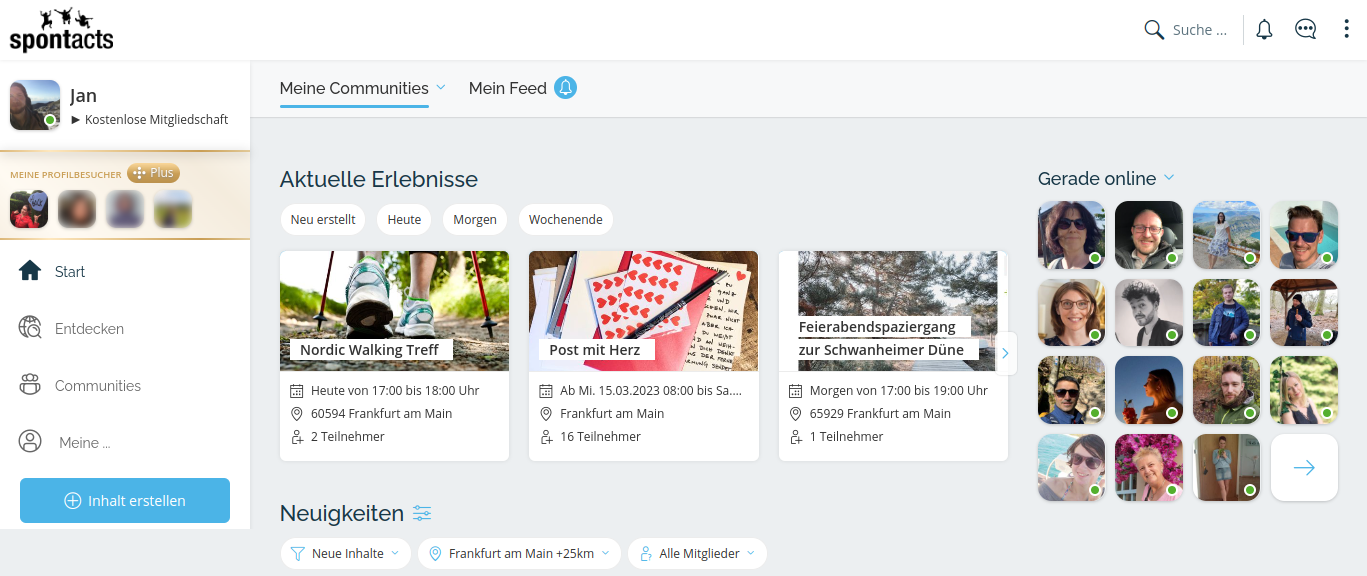
\includegraphics[width=\textwidth]{figures/jan/pic_spontacts.png}
    \caption[Startseite von Spontacts]{Startseite von Spontacts}
    \label{fig:spontacts}
\end{figure}

\paragraph{Selbstdarstellung}

Das Nutzerprofil auf Spontacts ähnelt dem anderer vergleichbarer Anwendungen und beinhaltet grundlegende Informationen wie den Namen, ein Profilbild, das Alter und den Wohnort. Es können jedoch auch weitere Angaben wie präferierte Kontakte für \textit{Freizeit}, \textit{Sport}, \textit{Reisen}, \textit{Tanzen} und \textit{Dating} oder zusätzliche Profilabschnitte (Hobbies, Interessen/Vorlieben usw.) hinzugefügt werden. Ein weiterer Abschnitt zeigt vergangene und zukünftige Aktivitäten des Nutzers sowie dessen Gruppenmitgliedschaften an.

\paragraph{Formen des Austausches}

Zur Interaktion mit anderen Benutzern können Beiträge in Spontacts erstellt werden. Diese Beiträge können je nach Art als einfacher Beitrag, als Aktivität oder als Frage/Diskussion verfasst werden und werden dann in Communities, Gruppen oder gegebenenfalls in Foren angezeigt. Wie gewohnt können sie kommentiert, gelikt und geteilt werden.

Die Communities sind eine Art Oberkategorie, die einen bestimmten Themenbereich (\textit{Ausgehen \&\ Party}, \textit{Essen \&\ Trinken}, \textit{Natur \&\ Umwelt} usw.) beschreiben und jedem Beitrag zugeordnet werden. Beim Erstellen einer Gruppe muss daher immer eine passende Community ausgewählt werden. Im Gegensatz zu den anderen vorgestellten Diensten sind Gruppen bei Spontacts das zentrale Feature der Anwendung. Sie ähneln in ihrem Funktionsumfang den Gruppen auf \acrshort{fb}.

Über die Beiträge hinaus können die Nutzer auch über den Chat eine private Unterhaltung führen. In diesem Chat können ausschließlich Textnachrichten ausgetauscht werden.

\paragraph{Recherche}

Um Beiträge, Veranstaltungen, Gruppen, Mitglieder und mehr zu entdecken, bietet Spontacts eine Suchfunktion mit spezifischen Filteroptionen je nach dem gesuchten Typ. Der Nutzer kann neben den allgemeinen Einstellungen wie Suchbegriff, Umkreis und Erstelldatum auch objektspezifische Kriterien wie Veranstaltungsdatum, Alter und ähnliches hinzufügen, um die Suche zu verfeinern.

Mitglieder können in die Kontakt- oder Merkliste aufgenommen werden, wenn sie für den Nutzer von Interesse sind. Die Merkliste ist eine private Liste, in die jedes Mitglied aufgenommen werden. Die Kontaktliste hingegen ist öffentlich und erfordert eine Bestätigung der Anfrage durch die betreffende Person. \\
Zusätzlich besteht die Möglichkeit, anderen Mitgliedern zu folgen, um ihre Aktivitäten besser verfolgen zu können. Wer wem folgt, kann in jedem Benutzerprofil eingesehen werden.

\paragraph{Neuigkeiten}

Um innerhalb der Plattform auf dem Laufenden zu bleiben, gibt es wie bei anderen Portalen ein Dashboard für Gruppen/Communities sowie einen Benachrichtigungs-Feed. Im Dashboard werden in der Rubrik \textit{Neuigkeiten} alle anstehenden Veranstaltungen und aktuellen Inhalte der Communities dargestellt. Unter der Rubrik \textit{Mein Feed} können hingegen alle Veränderungen in beigetretenen Gruppen eingesehen werden, wie beispielsweise neue Mitglieder und Veranstaltungen.\\
Der Benachrichtigungs-Feed enthält Informationen über neue Kontaktanfragen, Beiträge aus den Gruppen und Neuigkeiten über die Plattform.

\subsection{Strategische Ausrichtung}

Die drei Hauptwettbewerber weisen viele Gemeinsamkeiten auf, unterscheiden sich jedoch in ihrer strategischen Ausrichtung voneinander.

\acrshort{fb} ist eine sehr aktive Plattform, die sich darauf konzentriert, Menschen mit beliebigen Interessen, Themen und Bedürfnissen zu vernetzen, ohne dass der Nutzer dabei auf einen bestimmten geografischen Raum beschränkt ist. In letzter Zeit konnte keine intensive Weiterentwicklung der Plattform beobachtet werden, da sich das Unternehmen hauptsächlich der Entwicklung von zukünftigen Produkten im 3D-Umfeld widmet. Es ist daher lang- und mittelfristig keine Veränderung zu erwarten.

Nebenan.de ist der größte Konkurrent von \acrshort{dht}. Die Plattform ermöglicht es den Nutzern, sich in ihrer Nachbarschaft auszutauschen und zu vernetzen, wobei der Fokus auf der Stärkung der Gemeinschaft liegt. Eine große Herausforderung für Nebenan.de besteht darin, eine lebendige Community aufzubauen, die alle gesellschaftlichen Schichten und Altersklassen ansprechen.

Im Gegensatz dazu konzentriert sich Spontacts stark darauf, Menschen im privaten Bereich für gemeinsame Aktivitäten zu vernetzen. Die Plattform hat eine aktive Community, in der Nutzer Inhalte erstellen und an allen Veranstaltungen teilnehmen können, ohne harte lokale Einschränkungen wie bei nebenan.de. Darüber hinaus werden die Inhalte der Seite von lokal ansässigen Moderatoren betreut, die zusätzliche Veranstaltungen organisieren und durchführen. Strategisch setzt Spontacts zunehmend auf kostenpflichtige Accounts, die den Nutzern zusätzliche Funktionen wie verbesserte Filterfunktionen bieten sollen.

\subsection{Zusammenfassung}

Nach der Analyse der Konkurrenz wurde deutlich, dass die untersuchten Dienste ähnliche Funktionen wie Profile, Gruppen und Chats bereitstellen. Die Unterschiede zwischen den Features liegen eher in Nuancen, die von den jeweiligen Betreibern individuell gestaltet werden. \\
Die Plattformen unterscheiden sich jedoch in Bezug auf ihre Motivationen, Zielgruppen und geografischen Nutzerbereiche stark voneinander. Während einige Plattformen sich auf bestimmte Nachbarschaften beschränken, decken andere globale Communities ab. \\
Im Gegensatz dazu konzentriert sich \acrshort{dht} gezielt auf die Region/Gemeinde. Dadurch füllt \acrshort{dht} die Lücke zwischen \acrshort{fb} als weltweitem Akteur und nebenan.de mit Fokus auf die Nachbarschaft.

%Darüber hinaus hebt sich \acrshort{dht} von anderen Diensten durch die Einbindung von Vereinen und öffentlichen Einrichtungen ab, die die Plattform zur Kommunikation mit den Anwohnern nutzen können.

Ein weiterer Aspekt, der sich bei einem direkten Vergleich deutlich zeigt, ist die unterschiedliche Benutzerfreundlichkeit und Nutzerführung auf den verschiedenen Plattformen. Teils sind Inhalte schwer auffindbar und die zugrunde liegenden Konzepte sind nicht immer selbsterklärend. Um sicherzustellen, dass \acrshort{dht} für alle Altersgruppen verständlich ist, ist es unerlässlich, eine Plattform zu entwickeln, die einfach strukturiert und intuitiv zu bedienen ist.

Die Analyse zeigt anhand von nebenan.de und Spontacts, dass der Aufbau und die Etablierung eines sozialen Netzwerks viele Herausforderungen mit sich bringen. Als Vorreiter hat sich \acrshort{fb} in der Gesellschaft bereits stark etabliert und bietet mit einer breiten Palette von Features vielseitige Nutzungsmöglichkeiten für unterschiedliche Bedürfnisse. \\
Insbesondere für neue Plattformen stellt der Aufbau einer Community eine große Herausforderung dar. Als Newcomer müssen sie ohne bereits vorhandene Community und Content meist mit ähnlichen Funktionen wie Facebook die Nutzer überzeugen, dass ihre Plattform einen spürbaren Mehrwert im Vergleich zu Facebook bietet.
Gerade bei Plattformen, bei denen die Nutzer ausschließlich die Inhalte erstellen, gestaltet sich der Aufbau einer Community als besonders zäh, da neue Nutzer aufgrund mangelnder Inhalte schnell wieder abwandern können.\\
Daher ist es essentiell, dass kontinuierlich neue Inhalte zur Verfügung stehen, um sich zu etablieren. Spontacts setzt hierfür gezielt Moderatoren ein, um seinen Nutzern regelmäßig Angebote zu präsentieren. Alternativ kann die Bindung an ein Portal auch durch Angebote von Dritten erfolgen, wie zum Beispiel durch regelmäßige Informationen von Vereinen, Stadtverwaltungen oder Zeitungen, wie es bei \acrshort{dht} geplant ist. Zusätzliche Funktionen, wie ein Buchungsportal, können den Nutzern auch bei bestimmten Aktivitäten unterstützen.

\section{Anforderungsanalyse}
\label{sec:requirementanalysis}

\section{Visuelle Grundstrukturen}
\label{sec:visualstructure}
% \section{Visuelle Grundstrukturen}

Ein wichtiger Faktor für den Erfolg des Scrum-Teams ist es, dass jeder im Team das gleiche Verständnis über das zu entwickelnde Produkt hat. Die Sicherstellung dessen ist von hoher Bedeutung, um vermeidbaren Zeitfressern, wie lange Diskussionen, Missverständnisse, Nacharbeit und eine \ggf daraus hervorgehende Demotivation im Team entgegenzuwirken.
Darüber hinaus entstehen durch eine Visualisierung des Produktes Ideen und Lösungsansätze für Abläufe und Features, die frühzeitig im Entwicklungsprozess angesprochen, diskutiert und eingearbeitet werden können, ohne einen bemerkbaren Mehraufwand zu generieren.
Wireframes eignen sich für diese Aufgabe sehr gut, da sich diese schnell erstellen und abändern lassen und zugleich jedem Teammitglied einen ersten Entwurf des Produktes aufzeigen. Ein weiterer Vorteil besteht darin, dass bereits frühzeitig dem Kunden auf einfache Weise die ersten Designkonzepte vorgestellt werden können und dieser sein Feedback in einer frühen Entwicklungsphase mit einfließen lassen kann.

Das Erstellen von Wireframes beinhaltet zugleich, sich frühzeitig mit dem Aufbau und der Konzeption der Website auseinanderzusetzen. Aus diesem Grunde wird im weiteren Verlauf auch auf die Themen Seitenstruktur und Layout eingegangen.

\subsection{Grundlagen Seitenstruktur}

Die Seitenstruktur einer Website beschreibt die Art und Weise, wie die Inhalte einer Anwendung präsentiert, organisiert und verlinkt sind.

Die darzustellenden Informationen müssen daher nach Inhalt aufgeteilt und thematisch auf einzelnen Seiten organisiert werden. Jede Seite der Website besitzt somit ein klares Ziel, worüber sie informieren soll. Die einzelnen Seiten unterscheiden sich daher \bzgl ihres Ziels und Inhaltes. Jedoch existieren auf jeder Website eine Reihe von sogenannten Kernseiten, die oft aufzufinden sind. Klassische Seitentypen sind \bspw Startseite, Kontaktseite, Landingpage, Content- sowie Detailseiten.

Die Startseite, auch als Homepage bekannt, beschreibt die Seite, die den Startpunkt \bzw Ursprung einer Website darstellt. Von ihr aus kann über Verlinkungen zu allen Unterseiten navigiert werden.
Die Landingpage hingegen ist die erste Seite, die ein User wahrnimmt, wenn er von einem externen Link auf die Website geführt wird und eine Session beginnt. Die Landingpage wird oft für das Marketing hergezogen, um den Besucher für den Dienst zu begeistern und weitere Schritte anzuregen.
Die Contentseite hingegen gibt einen Überblick über die angebotenen Inhalte und verweist auf die zugehörige Detailseite, auf der die Inhalte detailliert aufgeführt sind.

Wie aus der Beschreibung der Seitentypen hervorgeht, werden die einzelnen Seiten zu unterschiedlichen Zeitpunkten oder in einer bestimmten Reihenfolge aufgerufen. Dies lässt sich auch als eine Art Hierarchie verstehen, die die einzelnen Seiten zueinander haben. Ob es sich hierbei um eine flache oder tiefe Hierarchie handelt, ist von der Navigationsstruktur abhängig. Allgemein werden häufig, wegen der besseren Orientierung, flache Seitenhierarchien empfohlen.

\begin{figure}
    \centering
    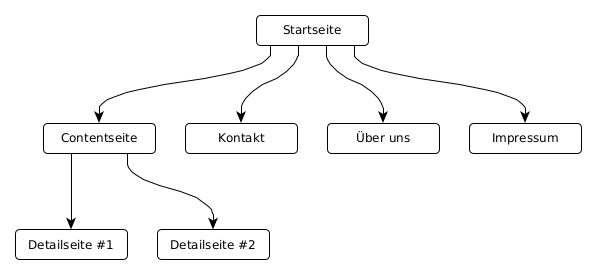
\includegraphics[width=\textwidth]{figures/jan/Wire_Hierarchie.png}
    \caption[Seitenstruktur einer Website]{Seitenstruktur einer Website}
    \label{fig:image}
\end{figure}

Die einzelnen Seiten einer Website unterscheiden sich jedoch \idR nicht vollständig voneinander. Sie folgen alle einem gleichbleibenden Aufbau. Dieses Grundgerüst einer Seite besteht oftmals aus einer Kopf- und Fußleiste und einem Inhaltsbereich. Die Kopf- und Fußleiste ist üblicherweise auf allen Seiten gleich ausgestaltet.

\begin{figure}
    \centering
    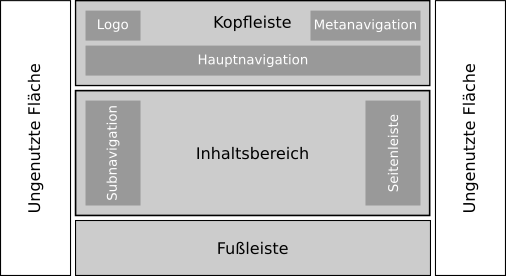
\includegraphics[]{figures/jan/Wire_Areas.png}
    \caption[Elemente einer Website]{Elemente einer Website}
    \label{fig:image}
\end{figure}

Der Kopfbereich einer Seite befindet sich im obersten Teil der Seite und umfasst das Logo, die Haupt- und Metanavigation. Der Kopfbereich wird häufig auch als Header bezeichnet.
Das Logo im Kopfbereich stellt ein wichtiges Erkennungs- und Differenzierungsmerkmal der Website dar und zielt auf das Erzeugen von Assoziationen mit der Website ab. Die Hauptnavigation gibt eine Übersicht über die verfügbaren Inhalte und stellt diese strukturiert dar. Die Hauptnavigation erweist sich für die Navigation als wichtigstes Element und wird häufig auffällig im oberen Bereich platziert. Eine weitere Navigationsleiste ist die Metanavigation, welche ergänzende Serviceinhalte wie \zB Accounteinstellungen der Seite verfügbar macht. Die Inhalte dieser Leiste haben keinen Bezug zu den Hauptthemen und werden daher gesondert aufgeführt.

Der Inhaltsbereich ist direkt unter dem Kopfbereich angeordnet und umfasst die zu vermittelnden Inhalte. Der Inhaltsbereich weist je nach Bedarf entweder nur die reinen Inhalte auf oder \ggf noch eine Subnavigation, die meist links angeordnet ist, sowie eine Seitenleiste (\engl Sidebar) für weiterführende Inhalte, die auf der rechten Seite untergebracht werden. Die zentralen Inhalte werden zwischen den Leisten, im sogenannten Inhaltsbereich, und meist nach Wichtigkeit absteigend sortiert aufgelistet.

Die untere Begrenzung der Internetseite bildet die Fußleiste (\engl Footer). Die Fußleiste beinhaltet meist Basisinformationen der Seite, ergänzende Inhalte oder auch \ggf weitere Navigationsmöglichkeiten.

Umschlossen werden die Seitenbereiche von einem umgebenden Block, der die ungenutzte Fläche der Website darstellt.

\subsection{Grundlagen Layout}
\subsection{Rastersystem}

Für die Überführung der ersten Skizzen in ein stimmiges Layout eignet sich die zur Hilfenahme eines Rastersystems. Ein Rastersystem stellt ein Netz mit Zeilen und Spalten dar, an welchen die Inhalte ausgerichtet und letztlich im Rastersystem platziert werden. Der Vorteil besteht darin, dass die Inhaltselemente und Einzelseiten in eine gleiche Struktur gebracht werden und die Seiten zunehmend abgestimmter und einheitlicher wirken. Das Raster wird lediglich für die Gestaltung herangezogen und sollte möglichst unauffällig oder dezent für den Endnutzer wirken,

Die Ausgangsbasis eines Rastersystems ist zu meist eine Leinwand mit definierten Abmessungen. Die Fläche wird in Spalten (\engl columns) unterteilt und \ggf wird zusätzlich noch zwischen den Spalten ein gleichbleibender Freiraum (\engl gutter) angelegt. Je höher die Spaltenanzahl gewählt wird, desto größer wird der gestalterische Spielraum, wobei der Nutzen des Rasters ab einer gewissen Anzahl zunehmend verschwindet.
In einem weiteren Schritt kann eine horizontale Unterteilung vorgenommen werden. Als Grundlage wird hier das sogenannte Baseline Grid verwendet, welches sich aus der Schriftgröße und dem Zeilenabstand zusammensetzt.
Die einzelnen Spalten und Zeilen können des Weiteren noch in Bereiche zusammengefasst werden, um ein modulares Rastersystem zu erstellen.
Die Website-Inhalte werden im Nachgang den Bereich zugeordnet und am Raster ausgerichtet.

\begin{figure}
    \centering
    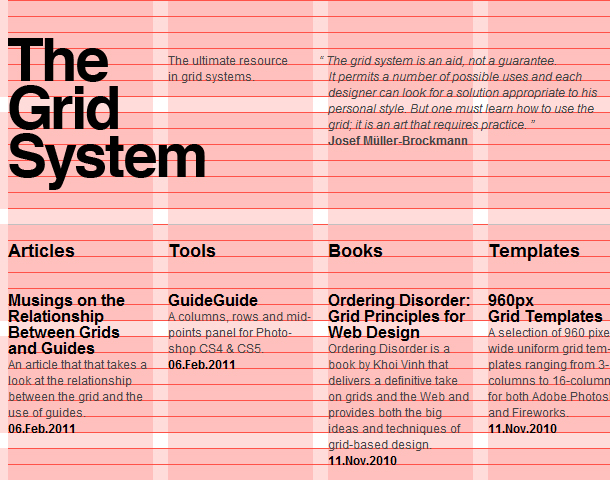
\includegraphics[width=0.6\textwidth]{figures/jan/Wire_Gridsystem.jpeg}
    \caption[Beispiel eines Rastersystems]{Beispiel eines Rastersystems}
    \label{fig:image}
\end{figure}

% ![Gridsystem](res/Wire_Gridsystem.jpeg)
% [//]: # (BILD Gridsystem: https://www.elmastudio.de/wp-content/uploads/2011/02/rastersysteme-webdesign-07.jpg)

\subsubsection*{Layouttypen}

Als es nur eine kleine Vielfalt an Endgeräten mit verschiedenen Auflösungen gab, wurde oft mit einem statischen Layout gearbeitet, welches für eine weit verbreitete Auflösung optimiert war. Heute lässt sich dieser Ansatz wegen der unüberschaubaren Menge an Geräten, die sich zudem stark in ihren Auflösungen unterscheiden, kaum noch heranziehen. Insbesondere schwer ist die Findung einer passenden Auflösung, die für einen Großteil der Geräte als ansprechend erscheint.
Heutzutage geht man hingegen nicht mehr von einer festen Breite bei der Layouterstellung aus, sondern erstellt Layouts, die sich je nach Auflösung individuell dem Gerät anpassen.

Während dieser Entwicklung sind verschiedene Layouttypen entstanden, die je nach Anwendungsfall zurate gezogen werden.

Das fixe Layout beschreibt einen Layouttyp, der mit festen Pixelwerten eine fixe Breite definiert. Bei einer passenden Auflösung werden alle Inhalte korrekt angezeigt. Je größer hingegen die Auflösung wird, desto größer wird der umgebende Block der Seite und viel ungenutzter Platz entsteht. Bei einer zu kleinen Auflösung tauchen horizontale Scrollbalken auf und die Inhalte erscheinen abgeschnitten \bzw werden nur noch unvollständig angezeigt.

\begin{figure}
    \centering
    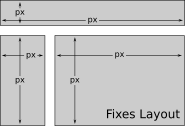
\includegraphics[scale=1.2]{figures/jan/Wire_Fixes-Layout.png}
    \hspace{0.05\textwidth}
    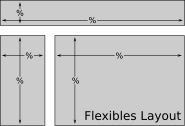
\includegraphics[scale=1.2]{figures/jan/Wire_Flexibles-Layout.png}
    \caption[Aufbau eines fixen und flexiblen Layouts]{Aufbau eines fixen und flexiblen Layouts}
    \label{fig:image}
\end{figure}

Das Gegenstück zum fixen Layout stellt das flexible Layout dar. Dieses passt sich allen Veränderungen unmittelbar an und behält dadurch zu jeder Zeit alle vorgegebenen Größenverhältnisse. Definiert wird es im Gegensatz zu den festen Pixelwerten mit relativen prozentualen Werten, wodurch es sich unterschiedlichen Varianten einer Website leicht anpassen kann. Der reine Layouttyp kommt jedoch eher selten zum Einsatz. Vielmehr lässt sich häufig eine Mischform aus fixem und flexiblem Layout vorfinden.

Eine weitere Layoutform ist das elastische Layout. Das elastische Layout verfolgt den Ansatz, dass sich die Inhalte einer Seite anpassen. Dieser Layouttyp ist besonders für Inhalte geeignet, die die vollständige Bildschirmbreite ausfüllen, was \bspw bei einer Produktpräsentation mit großformatigen Bildern und Videos der Fall ist. Die Inhalte müssen hierfür in der Lage sein sich automatisch flexibel anzupassen. Daher ist es für diese Form von Vorteil, wenn es eher wenige Inhalte zum Vorstellen gibt.

Auf Basis des flexiblen Layouts setzt das responsive Layout auf und erweitert die Möglichkeiten situationsgerecht ein passendes Layout für das Endgerät zur Verfügung zu stellen. Das responsive Layout besitzt als Erweiterung sogenannte Media-Queries, welche es ermöglichen beim Über- oder Unterschreiten fester Schwellwerte eine Veränderung der Ansicht zu starten und die Inhalte \bspw neu anzuordnen.

\subsection{Grundlagen Wireframes}

\subsubsection{Definition/ Inhalte}

Als Wireframe wird die schematische Darstellung von Inhalten und Elementen der Seitenoberfläche verstanden. Wireframes dienen insbesondere zur Konzeptionierung in der Planungsphase, um einerseits einen groben Entwurf für die Verteilung, Anordnung und Gestaltung von den Seitenelementen zu erhalten sowie zum anderen die Beziehungen zwischen den Seiten herzustellen.
Die Darstellung des Seitenlayouts ist zumeist eine skizzenhafte, in schwarz-weiß/ grau gehaltene Abbildung. Die einzelnen Bestandteile der Seite werden dabei durch einfache geometrische Formen verdeutlicht. Das Darstellen von Design, Farben, Schrift und Bilder ist kein Bestandteil der Methode. Ein fertiges Wireframe gibt dem Betrachter final Aufschluss über die Platzierung der Informationsinhalte, die Struktur und Navigation der Seite und die Interaktionselemente (Interface), mit welchen der Nutzer interagiert.
Die ausgearbeiteten Wireframes stellen weiter fort die Grundlage für die visuelle und funktionale Detaillierung des Produktes dar. Anschließende Schritte können \ua das Erstellen von Mockups oder Prototypen sein.

\subsubsection{Arten}

Wireframes werden allgemein in Low-Fidelity- und High-Fidelity-Wireframes unterschieden.
Low-Fidelity-Wireframes (LFW) stellen das klassische Verständnis von Wireframes dar, bei denen der Fokus allein auf dem funktionalen Design liegt. Die Seitenschemas werden mit einfachsten Formen und ohne konkrete Inhalte erstellt.
Die High-Fidelity-Wireframes (HFW) hingegen stellen die nächste Entwicklungsstufe für die Ausarbeitung des Designs dar. In ihr kommen zunehmend mehr und mehr Designkomponenten wie Farben, Typografie, Abstände, Icons, Text, Bilder und Grafiken zum Einsatz. In den Seiten werden zunehmend auch mehr reale Textlängen und Größenverhältnisse der Elemente und Inhalte mit einbezogen.

\begin{figure}
    \centering
    % [//]: # (BILD Beispiel LFW und HFW)
    % https://mentormate.com/blog/low-fidelity-wireframes-vs-high-fidelity-wireframes/
    % https://www.resolutesoftware.com/news/ux-wireframes/
    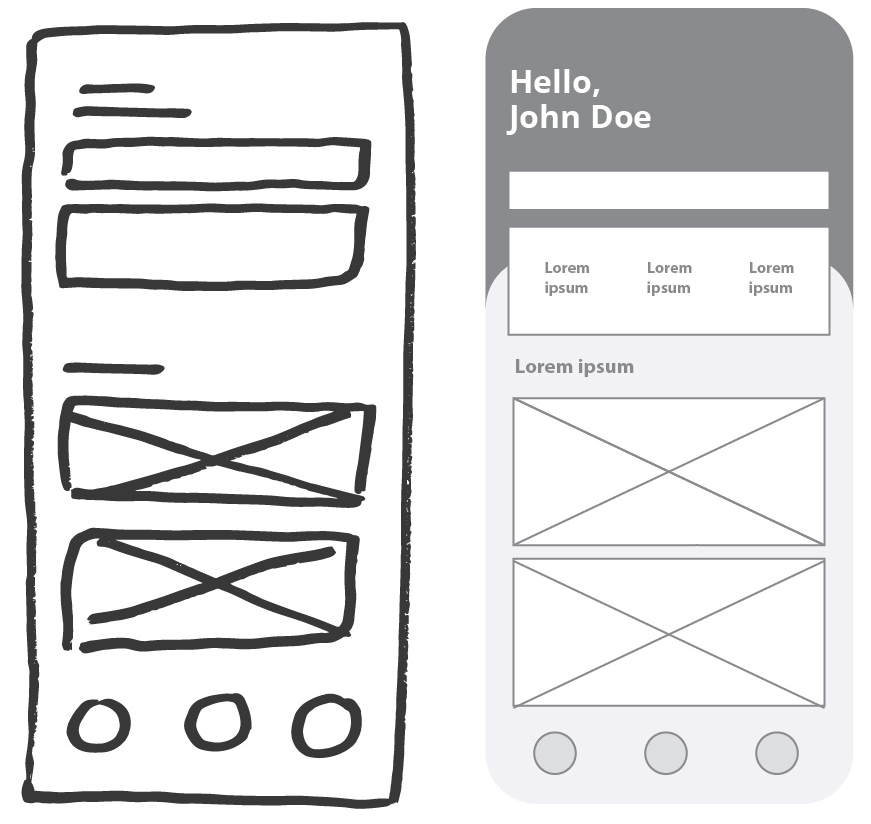
\includegraphics[scale=1]{figures/jan/Wire_Fixes-LFWvsHFW2.png}
    \caption[Beispielhafte Darstellung von LFW und HFW]{Beispielhafte Darstellung von LFW und HFW}
    \label{fig:image}
\end{figure}

\subsubsection{Abgrenzung}

Häufig werden im Zusammenhang mit Wireframes noch weitere visuelle Methoden in Verbindung gebracht. Weit verbreitet sind hier insbesondere Mockups und Prototypen. Diese Methoden verwenden jeweils Wireframes als Grundlage und zielen auf die zunehmende reale Veranschaulichung des zukünftigen Produktes.

Unter Mockups wird das Nachbilden eines Produktes oder auch ein maßstabsgerechtes Modell verstanden. Im Vordergrund der Methode steht das visuell-interaktive Design. Hierzu wird das Konzept der Wireframes übernommen und mit den Elementen der Benutzeroberflächen erweitert. Funktionale oder animierte Elemente sind nicht Bestandteil der Methode und werden nicht für einen Mockup aufgegriffen. Mockups werden im natürlichen Umfeld des Produktes dargestellt - zum Beispiel auf einem Gerätebildschirm. Das Ziel besteht darin das Produkt so echt wie möglich visuell nachzubilden, um dem Kunden ein reales Gefühl über die Erscheinung seines Produktes zu vermitteln.

% \begin{figure}
%     \centering
%     % [//]: # (Bild Mockup in Bildschirm)
%     \includegraphics[scale=0.25]{image.png}
%     \caption[]{image.png}
%     \label{fig:image}
% \end{figure}

Als Prototyp wird ein vereinfachtes Versuchsmodell des geplanten Produktes verstanden. Der Prototyp baut auf die Ergebnisse eines Mockups auf und erweitert dieses mit funktionalen Elementen, um die Interaktion eines Users mit dem Dienst simulieren zu können.
Ein klassisches Beispiel für einen Prototypen ist der Klick-Dummy. Ein Klick-Dummy ist ein teilweise interaktionsfähiges Demo einer Bedienoberfläche, welches alle relevanten Merkmale eines Produktes widerspiegelt und \ua zur Vorstellung oder für Testläufe genutzt werden kann.

\begin{figure}
    \centering
    % https://www.appschopper.com/blog/quick-guide-on-mobile-app-wireframe-vs-mockup-vs-prototype/
    % [//]: # (BILD Reihenfolge LFW - HFW - MockUp - Prototyp)
    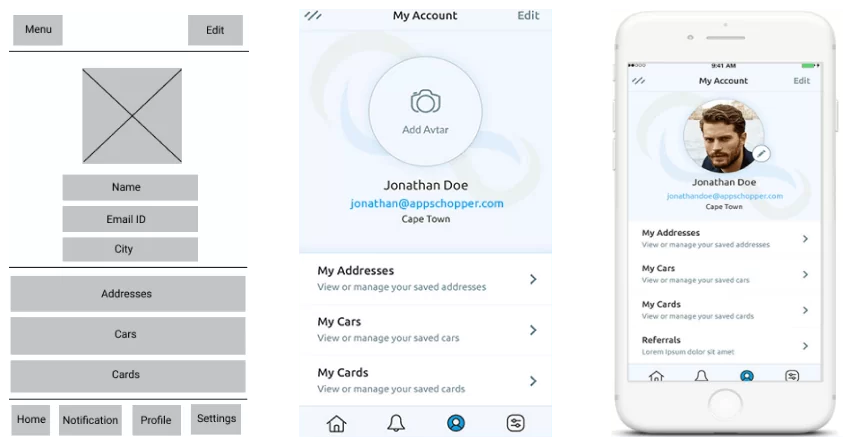
\includegraphics[scale=2]{figures/jan/Wire_Fixes-Wire-prototyp.png}
    \caption[Interationsschritte an einem Beispiel: Wireframe - Mockup - Prototyp]{Interationsschritte an einem Beispiel: Wireframe - Mockup - Prototyp}
    \label{fig:image}
\end{figure}

\subsection{Anwendung}
\subsubsection{Integration}

Die Wireframes wurden innerhalb des Projektverlaufes kontinuierlich für die Ausgestaltung und Kommunikation der User-Stories während des Backlog Refinement verwendet. Hierfür wurden in einer frühen Phase die jeweiligen User-Stories vom PO erläutert und ein erster Wireframe-Entwurf konzipiert. Erkenntnisse, die bereits während der Konzipierung entstanden, wurden an den PO übermittelt und nach Absprache noch während des Sprints direkt in die Wireframes aufgenommen.
Im Refinement dienten sie einerseits dem PO zur Vorstellung und Erklärung der User-Stories und andererseits zur Präzisierung und Detaillierung der Story im Team.
Die daraus neu gewonnenen Informationen wurden vom PO ins Backlog aufgenommen und erneut zum nächsten Refinement in die Wireframes eingearbeitet.

% \begin{figure}
%     \centering
%     % [//]: # (BILD Ablauf: Refinement 0 - 1 - 2 - 3, Feature A, B, C, Iteratives Vorgehen)
%     \includegraphics[scale=0.25]{image.png}
%     \caption[]{image.png}
%     \label{fig:image}
% \end{figure}

Neben der Definition und Veranschaulichung der jeweiligen Features wurden die Wireframes auch im Entwicklungsprozess herangezogen. In diesem wurden sie als gestalterischer Entwurf berücksichtigt und so weit wie es dem Entwickler möglich war, implementiert.

\subsubsection{Auswahl Tool}

Für die Erstellung von Wireframes stehen eine Vielzahl von verschiedenen Softwarelösungen zur Verfügung. Grundsätzlich lassen sich diese in desktop- und webbasierte Anwendungen unterscheiden. Für die Erstellung der Wireframes war es essenziell, dass diese leicht erstellt und angepasst werden können, \ggf auch paralleles Arbeiten möglich ist und dass das Teilen der aktuellen Entwürfe ohne zusätzlichen Aufwand geschieht. Anhand der Basisanforderungen konzentrierte sich die Auswahl zunehmend auf rein webbasierte Lösungen. Als Anbieter kristallisierte sich im weiteren Rechercheverlauf zunehmend Figma als ein passender Dienst heraus.

\begin{figure}
    \centering
    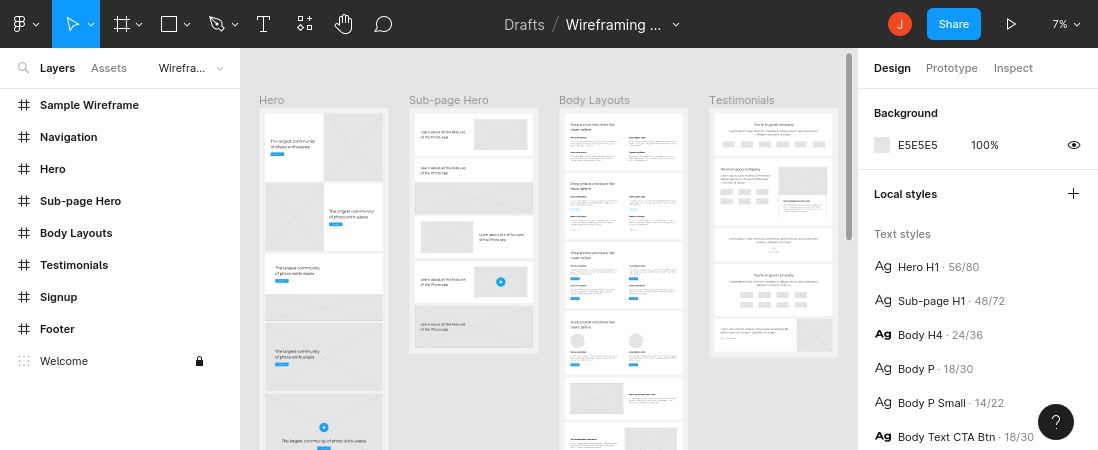
\includegraphics[width=\textwidth]{figures/jan/Wire_Figma.png}
    \caption[Figmas-Arbeitsumgebung]{Figmas-Arbeitsumgebung}
    \label{fig:figma}
\end{figure}

Figma ist eine Onlineanwendung, die sich auf die Erstellung von Wireframes, Mocks und Prototypen spezialisiert und sich in diesem Bereich etabliert hat. Gerade durch die Etablierung des Dienstes lässt sich schließen, dass es als Werkzeug ausgereift ist und die Erstellung einfacher Wireframes durchgängig unterstützt.
Für das Erstellen der Wireframes wurde sich auf die grundlegenden Funktionen von Figma beschränkt. Der verfolgte Ansatz während der Ausarbeitung mit Figma lag hierbei besonders auf der Beschränkung der wesentlichen Elemente, um die Kerninhalte der Features deutlich hervorzuheben. Eingesetzt wurden hierbei \ua zur Gestaltung die Elemente Rechtecke und Text sowie zur Orientierung und Ausrichtung der Inhaltselemente das Raster und die Gruppierfunktion.

\#\#\#\# Anforderungen an die GUI

Für die Ausarbeitung der Wireframes wurden vorab einige Anforderungen festgelegt, welche bei der Erstellung beachtet werden mussten. Die Anforderungen bezogen sich zum einen auf die Gestaltung der Oberfläche und zum anderen auf die technologiekonforme Gestaltung der Wireframes.

Eine wichtige Anforderung an die Plattform war es, die UI generationsübergreifend zu konzipieren. Aus diesem Ansatz heraus ließen sich die folgenden Ansprüche an die UI ableiten:

- Einfache und intuitive Seitengestaltung, um die Inhalte, den Funktionsumfang und die Bedienung schnell selbstständig erfassen zu können,
- Reduzierung der Inhalte auf das Wesentliche, um Verwirrungen/ Ablenkungen zu vermeiden,
- Flache Hierarchien, um direkte Zugriffe auf die gewünschten Inhalte zu ermöglichen.

Von der technologischen Seite her war es erforderlich, dass die erstellten Konzeptentwürfe sich auch mit den ausgewählten Web-Technologien umsetzen lassen. Die Entwickler sollten in die Lage versetzt werden die Entwürfe entweder mittels Eigenentwicklungen oder durch das Heranziehen von Bibliotheken umzusetzen, ohne auf größere Herausforderungen zu stoßen. Das Ziel war es darüber hinaus einen hohen Grad an Wiederverwendbarkeit der Komponenten zu erreichen.

\#\#\#\# Pages

Als geeigneter Wireframetyp wurde ein Hybrid aus LFW und HFW gewählt. Die erstellten Wireframes umfassten alle layouttypischen Bereiche wie Kopf-, Inhalts- und Fußbereich, deren Inhalte in Feldern vereinfacht symbolisiert wurden. Die einzelnen Felder beinhalteten Texte, Dummy-Blöcke \bspw für Bilder und Interaktionselemente (Buttons, Dialoge \usw).
Die Wireframes wurden sehr schlicht in Graustufen gehalten und ohne die Berücksichtigung von Designelementen (Farbe, Typografie \usw) erstellt. Für die regelmäßige Erstellung und Anordnung der Komponenten hat sich nach einigen Entwürfen die Leinwandbreite von 1160 Pixel mit einem Raster von 27×37 Pixel als vorteilhaft ergeben.

Wireframes wurden für die Seiten/ Dialoge

\begin{itemize}
    \item Landingpage,
    \item Registrierung,
    \item Dashboard,
    \item Chat,
    \item Profil,
    \item Accounteinstellungen,
    \item Merkzettel und
    \item Marktplatz
\end{itemize}

erstellt.

Die Art und Detailtiefe der Ausgestaltung zeigen exemplarisch die folgenden Wireframes.

\begin{figure}
    %\centering
    % https://latex.org/forum/viewtopic.php?t=29653
    \begin{minipage}[t]{0.5\textwidth}
        % [//]: # (BILD Wireframes)
        \includegraphics[page=2, width=1\textwidth]{figures/jan/wire_example.pdf}
        \caption[Startseite (DHT)]{Startseite (DHT)}
        \label{fig:image}
    \end{minipage}
    \begin{minipage}[t]{0.5\textwidth}
        % [//]: # (BILD Wireframes)
        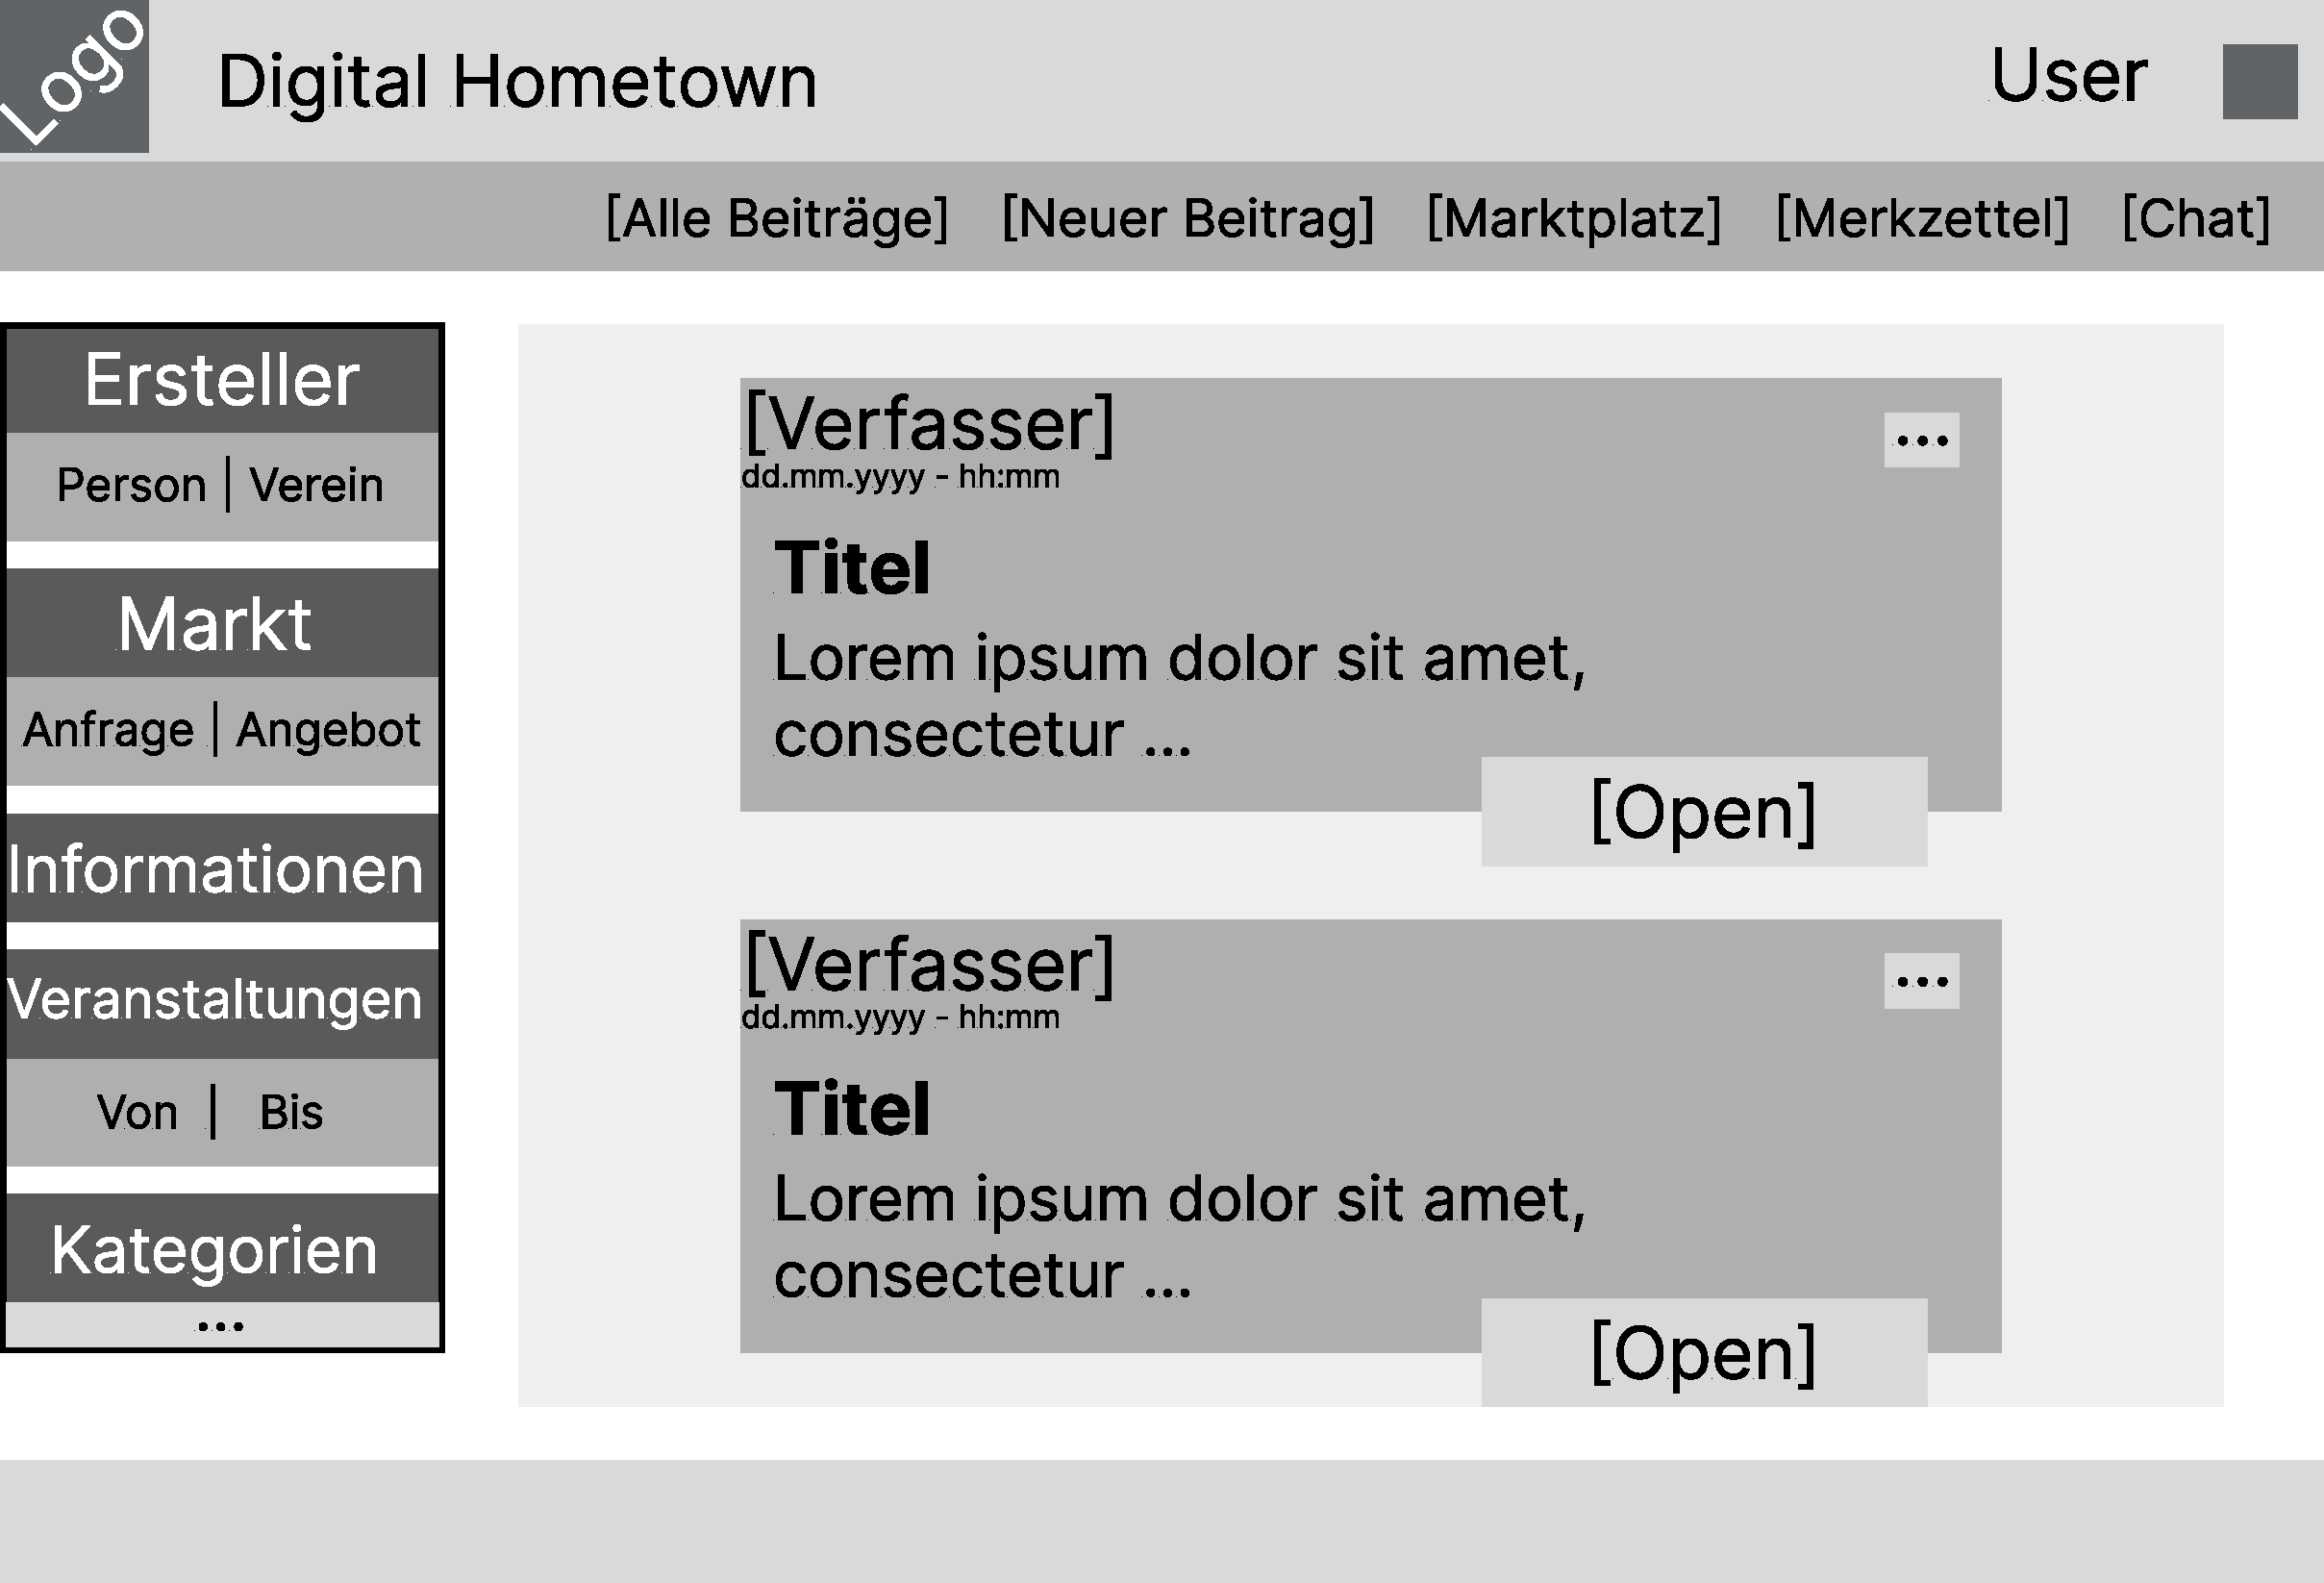
\includegraphics[page=1, width=1\textwidth]{figures/jan/wire_example.pdf}
        \caption[Marktplatz (DHT)]{Marktplatz (DHT)}
        \label{fig:image}
    \end{minipage}
\end{figure}


\section{Usabilityanalyse}
\label{sec:usabilityanalysis}

\chapter{Architektur}
\label{ch:architecture}

Auf Grundlage der Technologie Entscheidungen wurde folgende Architektur für das Projekt entwickelt.
Diese ist in folgender Abbildung dargestellt und wird in diesem Kapitel noch genauer erklärt:

\begin{figure}[ht!]
  \begin{centering}
    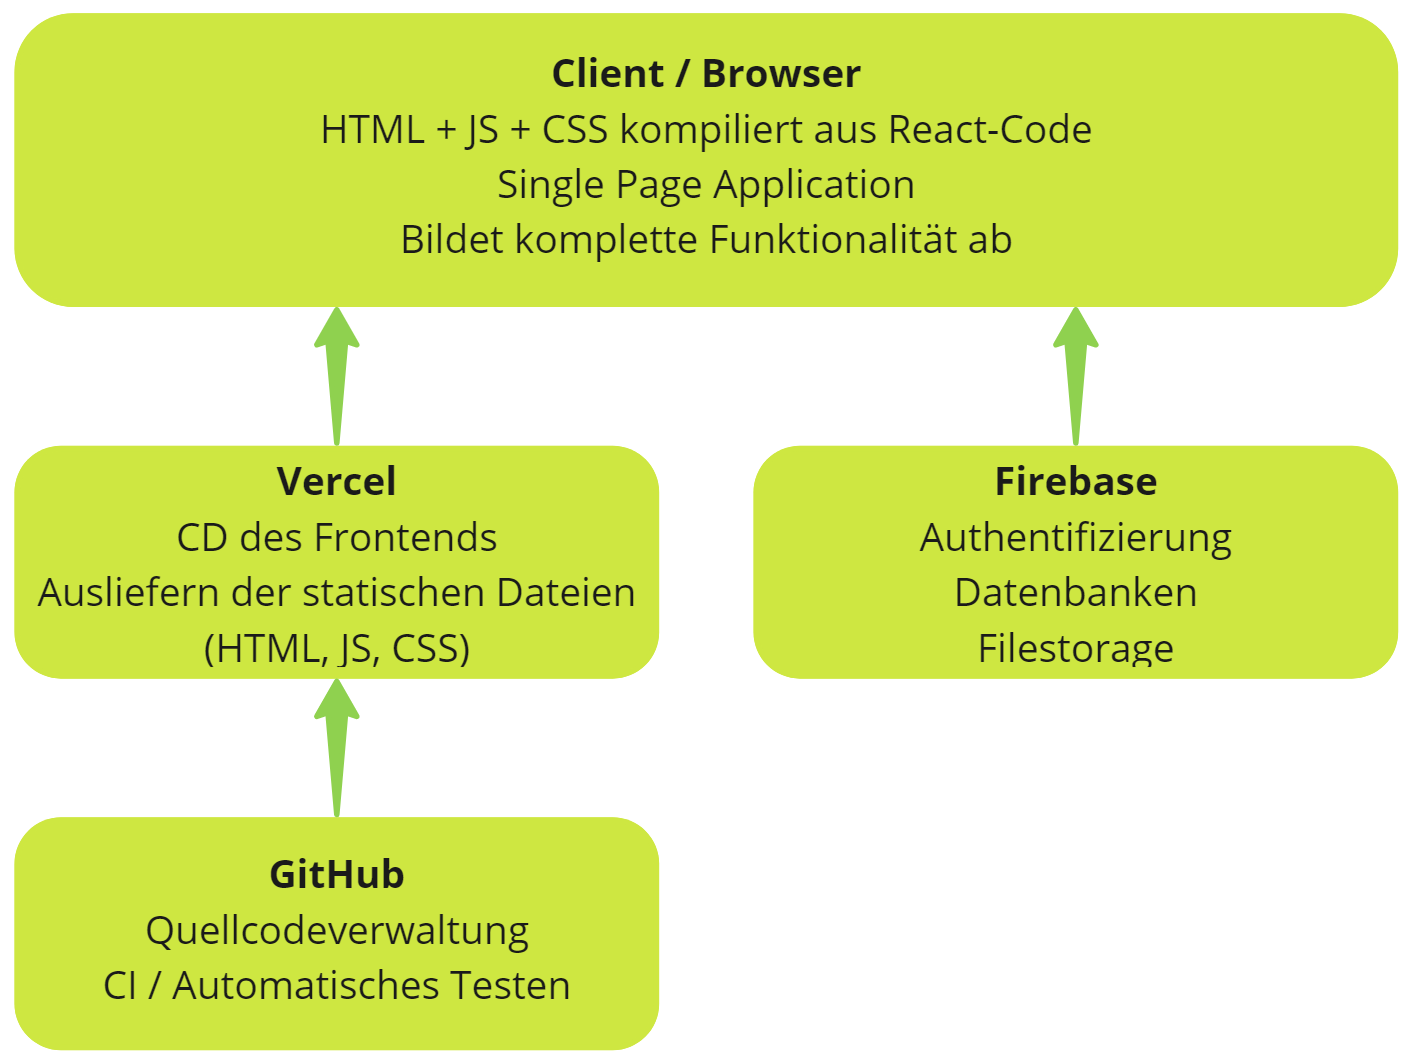
\includegraphics[width=.75\textwidth]{figures/architecture/architecture.png}
    \caption{Übersicht der technischen Softwarearchitektur}
    \label{fig:technicalArchitecture}
  \end{centering}
\end{figure}

Das Frontend wird in React entwickelt. Dieses enthält die Single Page Application (SPA) für die Benutzeroberfläche. Die gesamte Funktionalität wird in diesem Frontend implementiert.
Um im Team bei der Entwicklung effizient zusammenzuarbeiten, wir als Quellcodeverwaltungstool Git bzw. Github verwendet.
Wird eine Änderung am Quellcode veröffentlicht, werden automatisch die CI / CD Prozesse gestartet.
Sind die Tests erfolgreich, wird die neue Version über Vercel gehostet.

Wird der entsprechende Internetlink im Browser aufgerufen, erhält der anfragende Client (Browser) die statischen Dateien für die Benutzeroberfläche.
Der Browser führt das darin enthaltene Javascript aus, das ein dynamisches Laden der Inhalte der Datenbank (Firebase) ermöglicht.

\chapter{Technologien}
\label{ch:technical}

Für die Entwicklung eines Softwaresystems ist insbesondere bei der Implementierung entscheidend, welche Technologien verwendet werden.
Aus diesem Grund widmet sich diese Kapitel werden die technischen Aspekte der Plattform beschrieben.
Dabei werden die Technologien und Frameworks vorgestellt, die für die Entwicklung der Plattform verwendet wurden.

Die Plattform wurde mit den folgenden Technologien und Frameworks entwickelt:
\begin{itemize}
  \item \textbf{TypeScript} als Programmiersprache
  \item \textbf{React} als Frontend-Framework
  \item \textbf{\gls{mui}} als UI-Framework
  \item \textbf{Firebase} als Backend as a Service (\gls{baas})Plattform
  \item \textbf{Vercel} als Hosting-Plattform
  \item \textbf{Github} als Versionsverwaltungs-Plattform
  \item \textbf{Jira} als Projektmanagement-Plattform
\end{itemize}

Diese werden im Folgenden kurz vorgestellt.

\section{Grundlage für Technologieentscheidung}
\label{sec:technicalDecision}

Die einzige aus der Aufgabenstellung ersichtliche Vorgabe ist, dass das Softwareprodukt „Digital Hometown“ eine Plattform für den Austausch bieten soll.
Die Wahl der Technologie ist uns hierbei offengelassen.
Was daraus jedoch hervorgeht ist, dass es sich um eine für möglichst viele Nutzer verwendbare Web- oder Mobilanwendung handeln soll.
Insbesondere bei der Wahl einer Webanwendung, die dem Nutzer jeglichen Installationsaufwand erspart, ist die Hemmschwelle sehr gering, ein Softwareprodukt auszuprobieren.

Da, wie beschrieben, für eine solche Plattform des sozialen Austauschs eine ausreichend große Nutzerzahl entscheidend ist, fiel die Entscheidung schnell auf eine Webanwendung.
Obwohl beim aktuellen Stand der Plattform „Digital Dahoam“ nicht in erster Linie auf die Benutzbarkeit auf mobilen Endgeräten gelegt wurde, sei an dieser Stelle erwähnt, dass sich Webanwendungen mit etwas mehr Aufwand sehr gut auch für mobile Geräte wie Smartphones oder Tablets entwickeln lassen.
Der Fachbegriff hierfür ist die Umsetzung einer „Progressive Web-App“.

\section{TypeScript}
\label{sec:typescript}

TypeScript ist eine Erweiterung von Javascript, die statische Typisierung und Klassen hinzufügt.
Dadurch wird die Entwicklung von Software vereinfacht, da die Typisierung die Lesbarkeit des Codes verbessert und die Klassen die Wiederverwendbarkeit von Code ermöglichen.
Die Programmiersprache wird von Microsoft entwickelt und ist Open Source.\footnote{Vgl. TypeScript 2022 \cite{typescript2022}}

\subsection{Einsatz im Projekt}
\label{sub:typescriptUsage}

TypeScript wurde im Projekt verwendet, um die Entwicklung der Plattform zu vereinfachen. Der komplette Code der Website wurde mit TypeScript, HTML und CSS geschrieben, wobei TypeScript hierbei die Hauptrolle spielt.

\subsection{Grund für Technologieentscheidung}
\label{sub:typescriptReason}

Da TypeScript in großen Teilen der Javawelt inzwischen als de facto Standard ist um vor allem große Anwendungen sicher und effizient zu entwickeln, wurde diese Technologie für die Entwicklung der Plattform verwendet.
React (\ref{sec:react}), das größte Frontend-Framework der Welt, wird inzwischen auch in TypeScript entwickelt.\footnote{Vgl. TypeScript 2023 \cite{typescript2023}}

\section{React}
\label{sec:react}

React ist ein Open-Source Frontend-Framework, das von Facebook entwickelt wird.
Es ermöglicht die Entwicklung von Benutzeroberflächen für Webanwendungen.
Dabei wird die Benutzeroberfläche in einzelne Komponenten aufgeteilt, die unabhängig voneinander entwickelt werden können.
Diese Komponenten werden in einer \texttt{.\gls{jsx}} Datei definiert, die eine Kombination aus Javascript und HTML ist.
Die Komponenten werden in einer \gls{react} Anwendung in einer \texttt{.\gls{jsx}} Datei eingebunden.
In einer neueren Version, ist es auch möglich mit TypeScript zu arbeiten.
 Die neue Dateierweiterung für diese TypeScript ist \texttt{.\gls{tsx}}.
Diese Dateien werden dann in eine Javascript Datei kompiliert, die von einem Browser ausgeführt werden kann.\footnote{Vgl. React 2022 \cite{react2022}}

\subsection{Allgemeines in Bezug auf die Implementierung mit React}
\label{sub:reactGeneral}

React basiert auf dem Model-View-Controller Design Pattern. Der Browser Document Object Model (DOM) fungiert dabei als die View-Komponente. Die Model-Komponente, ist der Virtual DOM, das vom Controller (React) manipuliert wird.

\subsubsection{Einrichten und Starten der React-Anwendung}
\label{sub:reactSetup}

Für die Entwicklung von React-Anwendungen eignen sich alle moderne Entwicklungsumgebungen. Im Projektteam wurde sich auf den weitverbreiteten Texteditor „Visual Studio Code“ geeinigt. Neben einer Entwicklungsumgebung wird Node.js benötigt, um Javscript-Code auf der Entwicklungsmaschine ausführen zu können. Die notwendigen Abhängigkeiten werden mit dem Paketmanager „yarn“ installiert.
Mit dem in der Datei package.json definierten Alias yarn dev startet der lokale Node.js Entwicklungsserver automatisch, nachdem alle benötigten Pakete installiert wurden.
Handelt es sich um eine lauffähige Version, wird automatisch im Browser die Startansicht der entwickelten React-Anwendung geöffnet.

\subsubsection{React Components}
\label{sub:reactComponents}

React besteht aus Komponenten, die automatisch neu gerendert werden, wenn sich die Parameter der Komponente ändern.
Komponenten können als Functional- bzw. als Class-Komponenten implementiert werden.
Während die Verwendung von Class-Komponenten in älteren React-Versionen üblich war, wird in den aktuellen Versionen meist die funktionelle Implementierung verwendet.

\begin{lstlisting}[language=JavaScript, label=reactComponent, title={Beispiel einer React-Komponente}]
  function Component(props: {name: string}) {
    return <div>Hallo {props.name}!</div>
  }
\end{lstlisting}

\subsubsection{React Hooks}
\label{sub:reactHooks}
Die Komponenten bilden die Basis jeder React-Anwendung. Durch die React-Hooks wird es einer Komponente ermöglicht, dynamische Bestandteile und einen Zustand zu besitzen. Es gibt mehrere Hooks für verschiedene Anwendungsfälle und es lassen sich auch eigene Hooks definieren. Eines der wichtigsten React-Hooks ist useState. Durch useState wird es ermöglicht, eine Variable über ein oder mehrere Komponenten hinweg zu benutzen und manipulieren. Die Verwendung eines useState Hooks wird in Code 2 gezeigt. Hier wird auch ein weiterer wichtiger Hook aufgeführt. Der useEffect Hook ermöglicht es, auf die Änderung eines Zustands zu reagieren.

\begin{lstlisting}[language=JavaScript, label=reactComponentHooks, title={Beispiel einer React-Komponente mit Hooks}]
function Component() {
  // count ist der aktuelle Wert
  // setCount ist die Funktion, um den Wert zu ändern
  const [count, setCount] = React.useState<number>(0)

  React.useEffect(() => {
    // wird ausgeführt, wenn count sich ändert
    console.log("count changed")
  }, [count])

  return (
    <div>
      <p>{count} mal geklickt.</p>
      <button onClick={() => setCount(count + 1)}></button>
      Button
    </div>
  )
}
\end{lstlisting}

Es lassen sich beliebig viele Komponenten verschachteln. Das Durchreichen der Parameter wird bei größeren Projekten sehr aufwändig – insbesondere in Bezug auf die Wartbarkeit. Um dies zu entschärfen, gibt es weitere Konzepte wie der React Context, der im Folgenden beschrieben wird.

\subsubsection{React Context}
\label{sub:reactContext}

Der React Context ermöglicht es einen Zustand über mehrere Komponenten hinweg zu benutzen, ohne ihn mittels Parameter an alle Unterkomponenten durchzureichen. Man kann den React Context mit einer globalen Variable vergleichen.
Ein typischer Anwendungsfall für den React Context ist das Verwenden von Authentifizierungsdaten wie der Name über die gesamte Anwendung hinweg.

\subsection{Einsatz im Projekt}
\label{sub:reactUsage}

React wurde verwendet, um die gesamte Website aufzubauen.
Sie bildet alles ab, was der Benutzer sieht und mit der Plattform interagiert.

\subsection{Grund für Technologieentscheidung}
\label{sub:reactReason}

React wurde für die Entwicklung der Plattform verwendet, da es das meistgenutzte Frontend-Framework der Welt ist.
Außerdem gab es ein großes Interesse der verschiedenen Entwickler, sich in dieses Framework einzuarbeiten.

\begin{figure}[ht!]
  \begin{centering}
    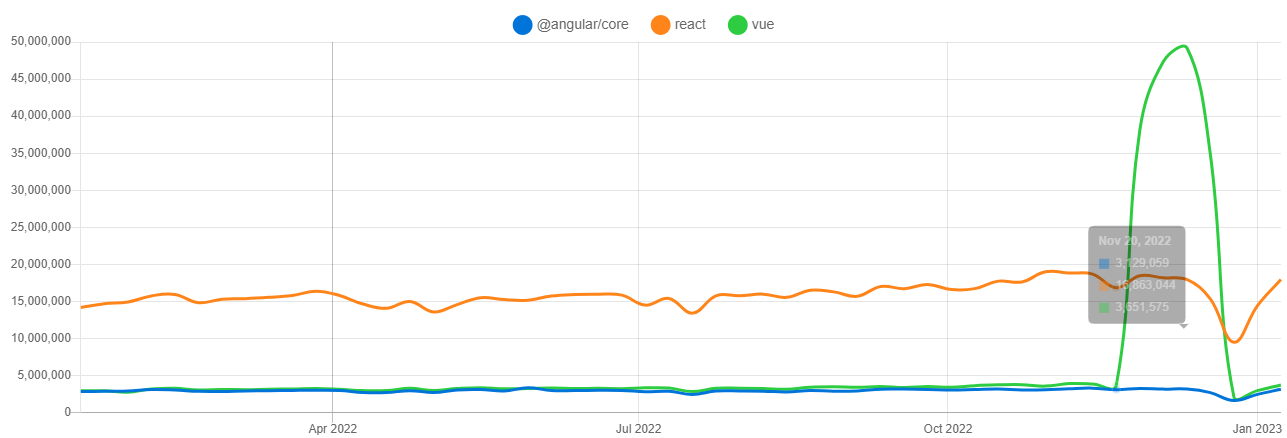
\includegraphics[width=.75\textwidth]{figures/technical/frontendFrameworks.png}
    \caption{Vergleich Downloadzahlen verschiedener Frontend Frameworks \cite{npm2023}}
    \label{fig:downloadFrontendFrameworks}
  \end{centering}
\end{figure}

\section{Material-UI}
\label{sec:material-ui}

Material-UI (kurz \gls{mui}) ist eine Bibliothek, die es ermöglicht, Komponenten aus dem Material Design zu verwenden.
Diese Komponenten sind konfigurierbar und können so an die eigenen Bedürfnisse angepasst werden.
Trotzdem entsprechen Sie alle einer einheitlichen Designsprache, die von Google entwickelt wurde. \footnote{Vgl. Google 2021 \cite{google2021}}

MUI bietet Komponenten für folgende Bereiche an:

\begin{itemize}
  \item \textbf{Navigation} – Komponenten für die Navigation.
  \item \textbf{Inputs} – Komponenten für die Eingabe von Daten.
  \item \textbf{Layout} – Komponenten für das Layout der Website.
  \item \textbf{Data Display} – Komponenten für die Anzeige von Daten.
  \item \textbf{Feedback} – Komponenten für die Rückmeldung an den Benutzer.
  \item \textbf{Surfaces} – Komponenten für Oberflächen.
  \item \textbf{Utils} – Komponenten für die Unterstützung.
\end{itemize}

Diese Bibliothek wird von Material-UI SAS. entwickelt und ist Open-Source auf Github verfügbar.
MUI bietet eine direkte Integration mit React. \footnote{Vgl. Material-UI 2022 \cite{mui2022}}

\subsection{Einsatz im Projekt}
\label{sub:material-uiUsage}

Da React nur sehr rudimentäre Komponenten für die Benutzeroberfläche bereitstellt, wurde MUI verwendet, um die Benutzeroberfläche zu gestalten.
Es bietet eine große Auswahl an Komponenten, die direkt in React verwendet werden können.

\subsection{Grund für Technologieentscheidung}
\label{sub:material-uiReason}

MUI vereinfachte die Gestaltung der Benutzeroberfläche, da es eine große Auswahl an Komponenten bietet, die direkt in React verwendet werden können.
Aus diesem Grund konnten die Entwickler schnell mit der Gestaltung der Benutzeroberfläche beginnen.

\section{Firebase}
\label{sec:firebase}

Firebase ist eine \gls{baas} Plattform, die die Bereitstellung von Backend-Funktionalität ermöglicht inklusive Datenbank, Authentifizierung, Datei-Upload, etc.
Dabei wird die Funktionalität in einzelne Module aufgeteilt, die unabhängig voneinander verwendet werden können.
Die Plattform wird von Google entwickelt\footnote{Vgl. Firebase 2022 \cite{firebase2022}} und besteht aus mehreren Komponenten, die nun kurz vorgestellt werden.

\subsection{Firebase Authentication}
\label{sub:firebase-authentication}

Firebase Authentication ist ein Modul von Firebase, das die Authentifizierung von Nutzern ermöglicht.
Dabei werden verschiedene Authentifizierungsmethoden unterstützt, wie z. B. E-Mail und Passwort, Google, Facebook, etc.
Außerdem ist es möglich eigene Authentifizierungsmethoden zu implementieren, sowie Nutzer über Telefonnummern zu authentifizieren.
Dabei können Nutzer auch in mehreren Geräten gleichzeitig eingeloggt sein.

Bis auf die Authentifizierungsmethode über Telefonnummern, die nur in den USA verfügbar ist, werden alle Authentifizierungsmethoden kostenlos angeboten. \footnote{Vgl. Firebase Authentication 2022 \cite{authentication2022}}

\subsection{Firebase Realtime Database}
\label{sub:firebase-realtime-database}

Firebase Realtime Database ist ein Modul von Firebase, das die Bereitstellung einer Datenbank ermöglicht.
Diese Datenbank ist eine NoSQL Datenbank, ähnlich wie MongoDB.
Hier werden die Daten nicht relational in Dokumenten gespeichert, sondern in einer Baumstruktur.
Updates in der Datenbank werden in Echtzeit an alle Nutzer gesendet, die sich mit der Datenbank verbinden.\footnote{Vgl. Firebase Realtime Database 2022 \cite{realtimedatabase2022}}

\subsection{Firebase Cloud Firestore}
\label{sub:firebase-cloud-firestore}

Firebase Cloud Firestore ist ein Modul von Firebase, das die Bereitstellung einer Datenbank ermöglicht.
Dabei wird die Datenbank in einzelne Dokumente aufgeteilt, die in einer Baumstruktur organisiert sind.
Firestore ist die Weiterentwicklung der Realtime Database und bietet einige Vorteile gegenüber dieser.
So ist die Datenbank in mehrere Regionen aufgeteilt, was die Verfügbarkeit erhöht.
Außerdem ist es möglich, die Datenbank in mehrere Projekte aufzuteilen, was die Sicherheit erhöht.
Abfragen in der Datenbank können mit Indexen optimiert werden, was die Performance verbessert. \footnote{Vgl. Firebase Cloud Firestore 2022 \cite{firestore2022}}

\subsection{Firebase Storage}
\label{sub:firebase-storage}

Firebase Storage ist ein Modul von Firebase, das die Bereitstellung von Datei-Upload ermöglicht.
Dabei können Dateien in einem Bucket gespeichert werden, das in einzelne Ordner aufgeteilt ist.
Der Datei-Upload kann über die Firebase Konsole oder über die Firebase SDK’s erfolgen.
Diese Funktion ist vergleichbar mit AWS S3 Buckets.\footnote{Vgl. Firebase Storage 2022 \cite{cloudstorage2022}}

\subsection{Einsatz im Projekt}
\label{sub:firebase-use}
Firebase wurde im Projekt für die Bereitstellung der Datenbank und der Authentifizierung verwendet.
Außerdem speichert es die Bilder, die von den Nutzern hochgeladen werden.


\subsection{Grund für Technologieentscheidung}
\label{sub:firebase-reason}
Durch Firebase konnte die Entwicklung der Backend-Funktionalität beschleunigt werden, da die Entwickler sich nicht um die Bereitstellung dieser Funktionalität kümmern mussten.

\section{Github}
\label{sec:github}

Github ist eine Plattform, die es ermöglicht, Softwareprojekte zu verwalten.
Diese Plattform wird von Github Inc. entwickelt. Github bietet eine direkte Integration mit Git.
Die wichtigsten Funktionen von Github sind in Tabelle \ref{tab:github} aufgeführt.\footnote{Vgl. Github 2022 \cite{github2022}}

\begin{table}[ht]
  \begin{tabularx}{\textwidth}{|l|X|}
  \hline
  \textbf{Funktion} & \textbf{Beschreibung} \\ \hline
  Versionsverwaltung & Github bietet Versionsverwaltung auf Grundlage von Git an. \\ \hline
  Projektmanagement & Anforderungen können als Issues angelegt und verwaltet werden. \\ \hline
  Dokumentation & Mithilfe von Markdown Wikis. \\ \hline
  Teamarbeit & In Form von Kommentaren, Reviews, etc. \\ \hline
  Hosting & Bereitstellung statischer Seiten. \\ \hline
  \gls{ci}/\gls{cd} & Automatisierte Tests und Deployment. \\ \hline
  \end{tabularx}
  \caption{Funktionen von Github}
  \label{tab:github}
\end{table}

\subsection{Einsatz im Projekt}
\label{sub:github-use}

Github wurde im Projekt für die Versionsverwaltung und \gls{ci} verwendet.
Die Versionsverwaltung wurde durch die Integration mit Git ermöglicht.
Außerdem wurden Github Actions benutzt, welches automatisierte Tests und andere Sanity-Checks ermöglicht.

\subsection{Grund für Technologieentscheidung}
\label{sub:github-reason}

Github wurde im Projekt eingesetzt, da es eine gute Integration mit Git bietet und somit die Versionsverwaltung vereinfacht.
Außerdem wurde durch die verfügbare \gls{ci} Funktionalität die Qualität des Codes verbessert und stetig getestet werden.
Die Entwicklungsgeschwindigkeit wurde dadurch vereinfacht.

\section{Vercel}
\label{sec:vercel}

Vercel ist eine Hosting-Plattform, die es ermöglicht, statische Webseiten zu hosten.
Diese Plattform wird von Vercel Inc. entwickelt.
Vercel bietet eine direkte zu \ref{sec:github} und erstellt neue Deployments und Builds, sobald ein neuer Commit in Github verfügbar ist.
Dies funktioniert auch mit mehreren Branches und Pull Requests. Jedes Deployment wird mit einer eigenen URL versehen, sodass mehrere Versionen der gleichen Webseite gleichzeitig verfügbar sind.
So können Pull Requests getestet werden, bevor sie in den Master Branch gemerged werden.\footnote{Vgl. Vercel 2022 \cite{vercel2022}}

\subsection{Einsatz im Projekt}
\label{sub:vercel-use}

Vercel wurde im Projekt für die Bereitstellung der Webanwendung verwendet.
Sobald bei Github ein neuer Commit verfügbar ist, wird automatisch ein neues Deployment erstellt.
Dies geschah für den main-Branch auf der Domain \url{https://dahoam.roser.dev} und für den dev-Branch auf der Domain \url{https://dev.dahoam.roser.dev}.
Jeder andere Branch bekam sein eigenes Deployment auf einer eigenen Domain, welche von Vercel erstellt wurde.

\subsection{Grund für Technologieentscheidung}
\label{sub:vercel-reason}

Vercel wurde verwendet, um die Bereitstellung der Webanwendung zu vereinfachen.
Nach Errichtung des Github Repositories und initialer Projekterstellung wurde die Integration mit Vercel in wenigen Klicks aktiviert und hostet seitdem kostenlos die Webanwendung.

\clearpage
\section{Jira}
\label{sec:jira}

Jira ist eine Plattform, die es ermöglicht, Softwareprojekte zu verwalten.
Diese Plattform wird von Atlassian entwickelt.

Die wichtigsten Funktionen von Jira sind in Tabelle \ref{tab:jira} aufgeführt.\footnote{Vgl. Atlassian 2023 \cite{attlassian2023}}

\begin{table}[ht]
  \begin{tabularx}{\textwidth}{|l|X|}
  \hline
  \textbf{Funktion} & \textbf{Beschreibung} \\ \hline
  Projektmanagement & Anforderungen können als Issues angelegt und verwaltet werden. \\ \hline
  Dokumentation & Mithilfe von Markdown Wikis. \\ \hline
  Teamarbeit & In Form von Kommentaren, Reviews, etc. \\ \hline
  \end{tabularx}
  \caption{Funktionen von Jira}
  \label{tab:jira}
\end{table}

\subsection{Einsatz im Projekt}
\label{sub:jira-use}

In Jira wurden die einzelnen User Stories verwaltet und bearbeitet, sowie in Sprints eingeplant.
Durch ein Kanbanboard wurden die einzelnen User Stories in den einzelnen Sprints angezeigt.
Jira bietet eine direkte Integration mit Github.

\subsection{Grund für Technologieentscheidung}
\label{sub:jira-reason}

Jira wurde verwendet, um die Verwaltung der User Stories zu vereinfachen.
Durch die direkte Integration mit Github wurden die einzelnen User Stories mit den dazugehörigen Commits verknüpft.
Dadurch konnte die Entwicklung der einzelnen User Stories nachvollzogen werden.
Außerdem ist es ein sehr simples Tool, welches für die Verwaltung von User Stories sehr gut geeignet ist.

\chapter{Implementierung}
\label{ch:implementation}

In diesem Kapitel wird die Implementierung der Anwendung beschrieben.
% Hierbei wird exemplarisch auf zwei wichtige Funktionen der Anwendung eingegangen.
% Diese sind die Verwaltung des Benutzerprofils und die Erstellung und Anzeige von Beiträgen.

Da der komplette Code und viele Screenshots den Rahmen dieses Kapitels sprengen würden, wird in den einzelnen Kapiteln nur ein Auszug gezeigt.
Den kompletten Code findet man direkt im Github Repository unter \url{https://github.com/Jonasdero/digital-hometown-frontend}.

 \section{Landing Page}
 \label{sec:landing_page}
 
Bei dem Aufruf der Plattform \glqq Digital Dahoam\grqq \ wird der Nutzer auf die Landing Page (s. \autoref{fig:landing_page}) weitergeleitet. Diese ist abhängig davon, ob der Nutzer eingeloggt ist oder nicht.

Auf der Landing Page wird die Vision der Plattform vorgestellt. Bei dem Projekt \glqq Digital Dahoam\grqq \ geht es darum, dass sich Menschen in der Nachbarschaft vernetzen können. Die Plattform soll zudem die Menschen dazu motivieren, anderen zu helfen, bzw. selbst um Hilfe zu bitten. Insbesondere für neu zugezogene Menschen soll die Plattform eine Möglichkeit sein, die Umgebung zu entdecken und interessante Vereine kennenzulernen.

\begin{figure}[!htb]
  \centering
  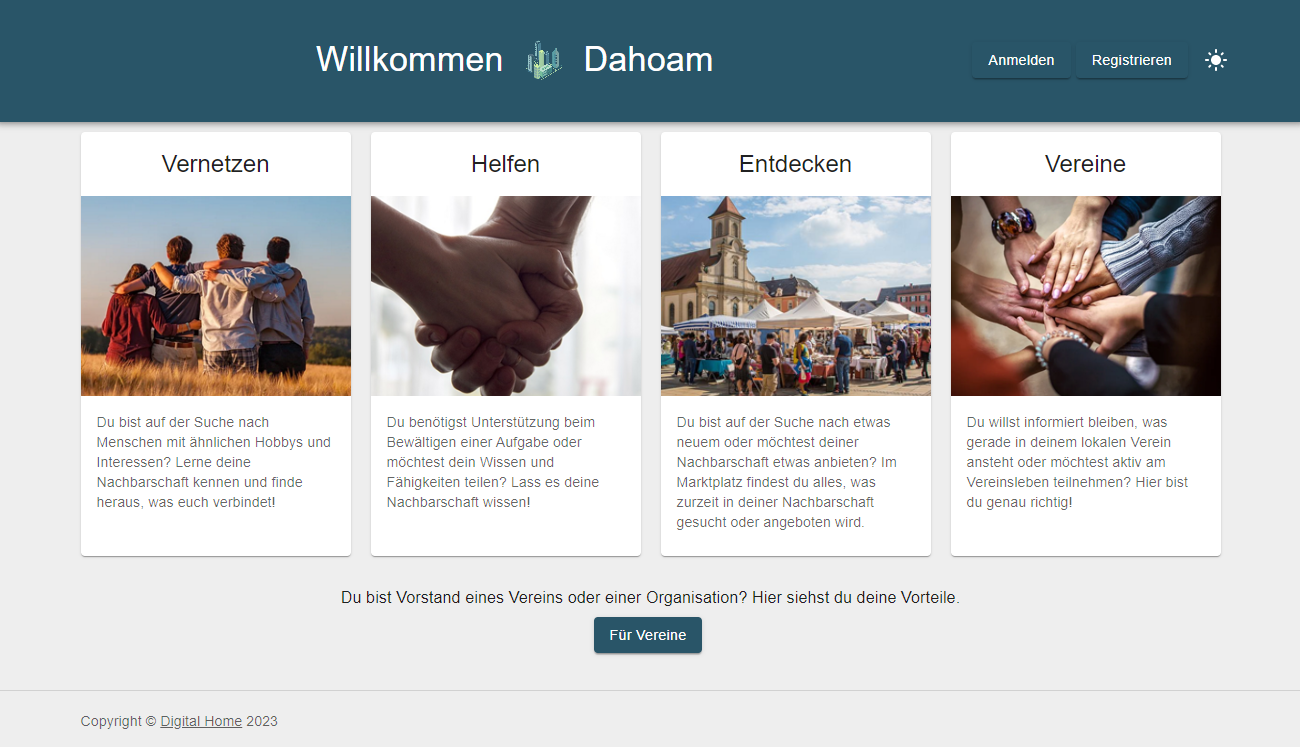
\includegraphics[width=.9\textwidth]{figures/boas/21_landing_page.png}
  \caption[]{Bildschirmaufnahme der Startseite für nicht eingeloggte Nutzer}
  \label{fig:landing_page}
\end{figure}

Will sich ein Benutzer bspw. ein Vereinsvorstand mit seinem Verein registrieren, kann er über den Button \glqq Für Vereine\grqq \ zur Landing Page für Vereine navigieren. Über die Landing Page für Vereine kann der Vorstand seinen Verein bei der Plattform registrieren oder sich einloggen (s. \autoref{fig:landing_page_verein}). Der Inhalt der Landing Page beschreibt, welche Vorteile die Plattform für Vereine bietet.

\section{Profil}
\label{sec:profile}

Die Profile eines Nutzers sind in der Anwendung sehr wichtig.
Jeder Nutzer verwaltet sein eigenes Profil, welches er mit anderen Nutzern teilt.
Dazu gehören Informationen wie Name, E-Mail-Adresse, Geburtsdatum, Geschlecht und ein Profilbild.
Damit andere Nutzer die Informationen des Profils sehen können, muss das Profil öffentlich sein.
Zudem sollen Benutzer der Anwendung durch Interessen, Profilbilder und persönliche Beschreibungen voneinander unterscheidbar sein und sich so besser vernetzen können.
Um sich mit anderen Nutzern zu verbinden, ist es wichtig, dass diese Informationen in der Anwendung gespeichert werden.

Außerdem soll die soziale Interaktion zwischen Nutzer ermöglicht werden.
Dazu gehören Funktionen wie das Folgen von anderen Nutzern oder auch das Schreiben von Nachrichten zwischen zwei Nutzern oder in Gruppen.
Dies soll direkt vom Profil eines Nutzers aus möglich sein.

\begin{figure}[ht!]
  \begin{centering}
    
\includegraphics[width=1\textwidth]{figures/implementation/profile-header.png}
    \caption{Übersicht eines Benutzerprofils}
    \label{fig:userProfileHeader}
  \end{centering}
\end{figure}

Hier sieht man die verschiedenen Informationen, die ein Nutzer in seinem Profil angeben kann.
In den nächsten Seiten wird die Implementierung dieser Funktionen beschrieben.
Diese wird aufgeteilt in die verschiedenen Bereiche: \textit{Anmeldung \& Registrierung}, \textit{persönliches Accountmanagement}, \textit{Profilseite \& Profilbilder} und \textit{blockierte Nutzer}.

\subsection{Anmeldung \& Registrierung}
\label{sec:login}

Den Nutzern wird die Möglichkeit gegeben, sich mit einer E-Mail-Adresse und einem Passwort anzumelden oder eine direkte Anmeldung über OAuth mit Google zu nutzen.
Dies wird beides durch die Firebase Authentication API ermöglicht.

Sobald ein Nutzer sich registriert hat, wird von Firebase intern ein Benutzerprofil erstellt, welches wichtige Nutzermetadaten und Authentifizierungsinformationen enthält.
Außerdem wird bei der Anmeldung über Google das Profilbild mit in Firebase gespeichert.
Die Anmeldemaske sieht wie folgt aus:

\begin{figure}[ht!]
  \begin{centering}
    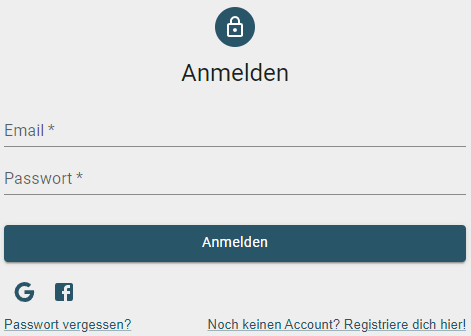
\includegraphics[width=.75\textwidth]{figures/implementation/anmeldemaske.png}
    \caption{Anmeldemaske}
    \label{fig:login}
  \end{centering}
\end{figure}

Um diese Daten in der Anwendung zu speichern, wird ein eigener Benutzerdatensatz angelegt, sobald ein Nutzer registriert wurde und Daten aus dem internen Benutzerprofil von Firebase mit übertragen.
Hierbei wird unterschieden, ob der aktuelle Benutzer ein normaler Nutzer oder ein Verein ist.
Diese werden in unterschiedlichen „Collections“ gespeichert.
Bei der Anmeldung wird dann geprüft, welchen Typ der Benutzer hat und die Daten entsprechend geladen.
Dadurch kann mit einer Datenstruktur gearbeitet werden, die für beide Typen geeignet ist.
Andere Ansichten basieren dann häufig auf der Unterscheidung zwischen Nutzern und Vereinen.
Die Struktur des Datensatzes kann man in Abbildung \ref{fig:firestoreUser} sehen.

\section{Authentifizierung}
\label{sec:authentifizierung}

Essentiell für ein soziales Netzwerk ist es, dass die Benutzer sich mit einem Profil registrieren können. Wie das im Detail funktioniert und wie die Authentifizierung implementiert wurde, wird in diesem Kapitel beschrieben.

\subsection{Verwendung des \glqq Firebase-Authentication\grqq-Services}
\label{sec:firebase_authentifizierung}
Die Implementierung der Authentifizierung wird mit dem Backend-as-a-Service-Anbieter Firebase durchgeführt. Firebase bietet eine Schnittstelle, die es ermöglicht, Profile anzulegen sowie den Anmelde- und Registrierungsprozess mit wenigen Zeilen Code zu implementieren.

Durch die verschiedenen Authentifizierungsmethoden, die Firebase anbietet, kann der Nutzer sich mit E-Mail und Passwort, Google oder Facebook anmelden. Die Authentifizierungsmethoden können einfach in der Firebase-Konsole aktiviert werden.

Es wird zu dem die Möglichkeit geboten, dass Nutzer, die ihre Zugangsdaten vergessen haben, eine E-Mail mit einem Link zum Zurücksetzen des Passworts erhalten.

Die Beschriebenen Funktionen decken also einen standardmäßigen Anmelde- und Registrierungsprozess ab.

\subsection{Zugriff auf die Profilinformationen}
\label{sec:zugriff_profilinformationen}
Wie bei der React-Einführung beschrieben, ist es aufwendig, Informationen wie die des Profils über die gesamte Anwendung hinweg durchzureichen. Dafür wurde auch bereits die Möglichkeit des React Contexts vorgestellt. Da dieses Konzept auch für die Profilinformationen eingesetzt wird hier nochmal ein Beispiel der Implementierung gezeigt.

Das in \autoref{lst:authcontext} stellt das Interface des Contexts dar, das für alle Components befüllt wird. Die Profilinformationen sind im Attribute \texttt{currentUser} gespeichert.

\begin{lstlisting}[language=JavaScript, caption=Auszug aus dem Interface des Authentifizierungscontexts, label={lst:authcontext}]
interface AuthContextI {
  currentUser: User | Club | undefined | null
  setCurrentUser: React.Dispatch<React.SetStateAction<User | Club | undefined | null>>
  logOut: () => void
  logIn: (email: string, password: string) => void
  signUpWithEmail: (email: string, password: string, displayName: string, isOrg: boolean) => Promise<void>
  signUpOAuth: (providerName: "google" | "facebook", isOrg: boolean) => void
  // usw.
}
\end{lstlisting}

% \autocite{attlassian2023}
Um den Vorteil des Contexts für die Codequalität hervorzuheben wird in \autoref{lst:authcontext_impl} dargestellt, wie einfach es möglich ist, die zentral befüllten Attribute in einer beliebigen React-Komponente zu verwenden.
Hierbei wird das Prinzip der Higher-Order-Components (HOC) genutzt, das zuvor implementiert wurde. Es ist lediglich notwendig, die implementierte Komponente mit dem HOC \texttt{withAuth} zu umschließen. Dieses HOC stellt der jeweiligen Komponente die Attribute des Contexts als Props zur Verfügung.

\begin{lstlisting}[language=JavaScript, caption=Verwendung des Authentifizierungscontext-HOCs, label={lst:authcontext_impl}]
function SignOut({ logOut }: AuthContextI) {
  useEffect(() => logOut(), [logOut])
  return <Navigate to="/" />
}

export default withAuth(SignOut)  
\end{lstlisting}

Das Component \texttt{SignOut} bekommt hier beispielsweise durch das HOC automatisch die Funktion \texttt{logOut} als Prop übergeben, die dann zum Ausloggen des Benutzers verwendet wird.

\subsection{Authentifizierungsprozess}
\label{sec:authentifizierungsprozess}

Im folgenden wird nun anhand von Bildschirmaufnahmen gezeigt, wie der Authentifizierungsprozess abläuft.

Beim Klick auf den Registrieren-Button der Landing-Page wird man auf eine Seite weitergeleitet, über die Benutzername, Email und Passwort eingegeben werden können (s. \autoref{fig:registrierung}). Fehlerhafte Eingaben der E-Mail-Adresse, sowie die redundante Eingabe des Passworts werden hierbei validiert.

\begin{figure}[!htb]
  \centering
  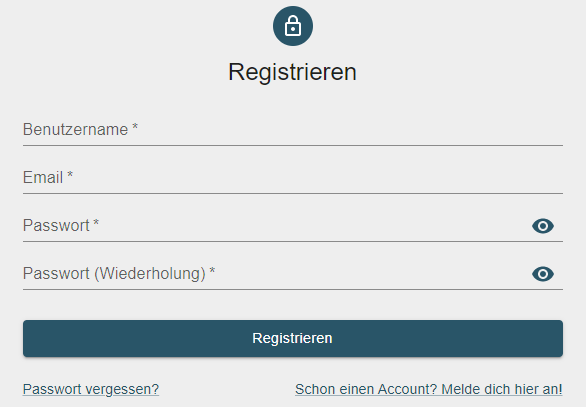
\includegraphics[width=0.5\textwidth]{figures/boas/21_registrieren.png}
  \caption[]{Registrierungsseite}
  \label{fig:registrierung}
\end{figure}

Nach der erfolgreichen Registrierung des Nutzers, wird er zunächst auf eine Seite geführt, auf der er seine Profilinformationen um das Geburtsdatum und die Postleitzahl ergänzen kann (s. \autoref{fig:registrieren_profilinfo}).

\begin{figure}[!htb]
  \centering
  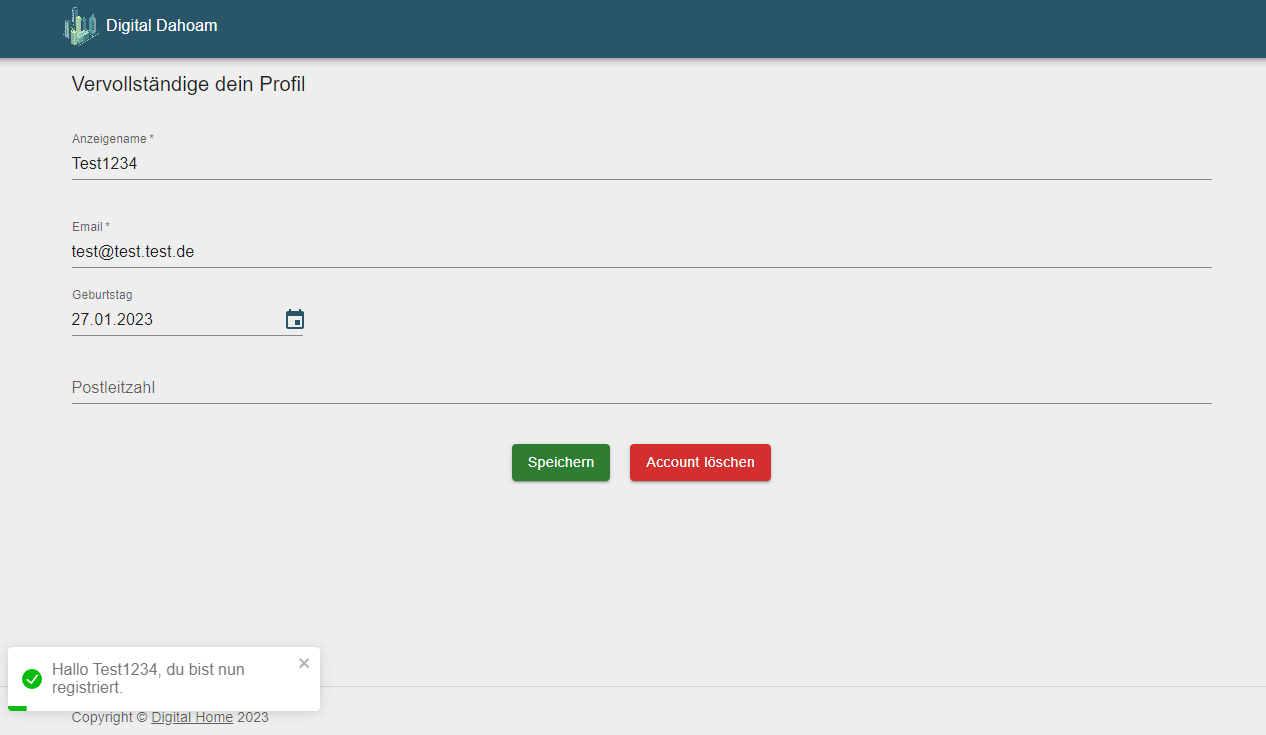
\includegraphics[width=0.9\textwidth]{figures/boas/21_registrieren_profilinfo.png}
  \caption[]{Ergänzen der Profilinformationen beim ersten Anmelden}
  \label{fig:registrieren_profilinfo}
\end{figure}

Nach der erfolgreichen Registrierung wird der Nutzer auf sein Profil weitergeleitet, wo er u. a. Interessen hinterlegen kann, um von Nutzern gefunden zu werden, welche die gleichen Interessen haben. Details hierzu sind dem Projektbericht von Jonas Roser zu entnehmen.

Eine besonders einfache Möglichkeit, sich bei der Plattform zu registrieren, bzw. anzumelden ist die Authentifizierung über Google. Beim Klick auf das Google-Icon öffnet sich direkt der Google-OAuth-Dialog (s. \autoref{fig:anmelden_google}). Dies steigert die Usability der Plattform, da der Nutzer nicht mehr die E-Mail-Adresse und das Passwort eingeben muss.

\begin{figure}[!htb]
  \centering
  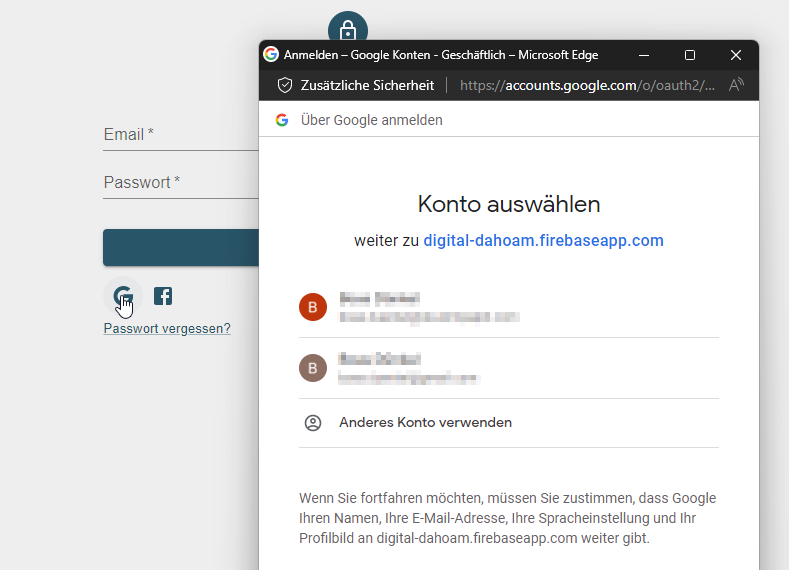
\includegraphics[width=0.6\textwidth]{figures/boas/21_anmelden_google.png}
  \caption[]{Authentifizierungs-Dialog beim Anmelden mit Google}
  \label{fig:anmelden_google}
\end{figure}

Wenn der Nutzer sich mit einer E-Mail-Adresse registriert hat, kann er sich auf folgender Seite anmelden (s. \autoref{fig:anmeldung}).

\begin{figure}[!htb]
  \centering
  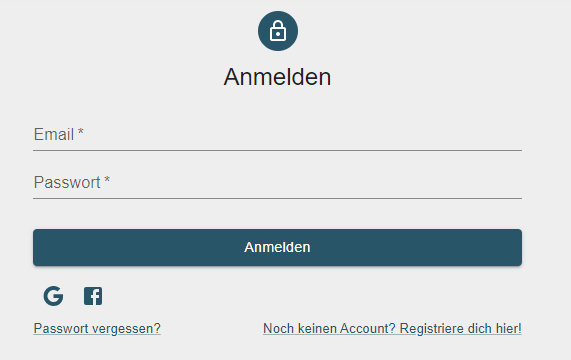
\includegraphics[width=0.5\textwidth]{figures/boas/21_anmelden.png}
  \caption[]{Anmeldeseite}
  \label{fig:anmeldung}
\end{figure}

\clearpage

\subsection{Persönliches Accountmanagement}
\label{sec:accountmanagement}

Um die Daten des Benutzerprofils zu verwalten, gibt es eine Seite, auf der der Nutzer seine persönlichen Daten ändern kann.
Diese werden dann in der Anwendung aktualisiert und in der Datenbank gespeichert. Er hat hier die Möglichkeit seinen Namen, seine E-Mail, sein Geburtsdatum und seine Postleitzahl zu ändern.
Hier kann außerdem der komplette Account gelöscht werden, um die Daten des Nutzers zu löschen.

\begin{figure}[ht!]
  \begin{centering}
    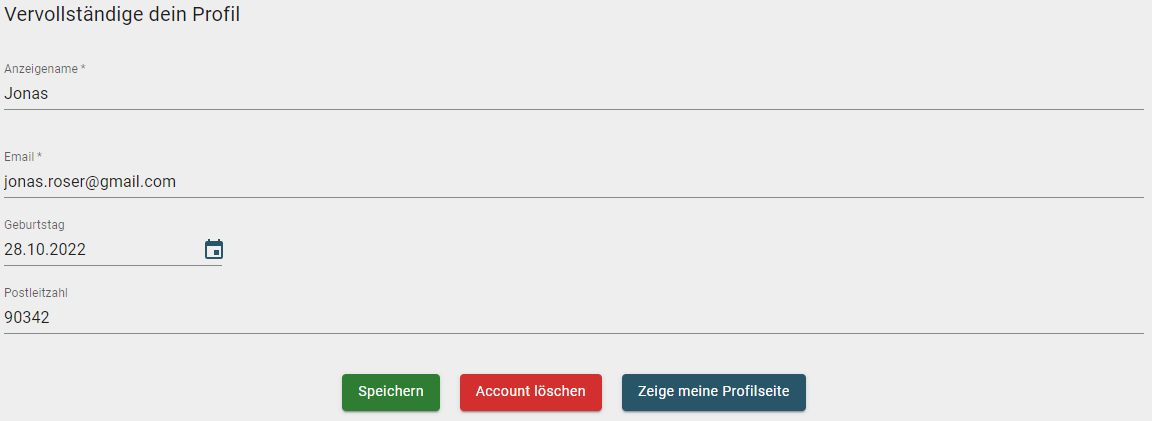
\includegraphics[width=1\textwidth]{figures/implementation/userSettings.png}
    \caption{Benutzereinstellungen}
    \label{fig:userSettings}
  \end{centering}
\end{figure}

\subsection{Profilseite \& Profilbilder}
\label{sec:profilepictures}

Auf der Profilseite des Nutzers kann er seine persönlichen Daten einsehen und bearbeiten. Hier können Interessen und eine Beschreibung hinzugefügt werden.
Außerdem kann er sein Profilbild ändern, indem er auf das Profilbild oder auf den Knopf mit der Kamera klickt.
Dies wird dann im Firebase Storage gespeichert und in der Datenbank verlinkt.

Das Ganze ist so aufgebaut, dass Nutzer zwischen einer Vorschau, also der Sicht, die auch andere Nutzer von seinem Profil sehen und der Bearbeitungssicht unterscheiden können.

\begin{figure}[ht!]
  \begin{centering}
    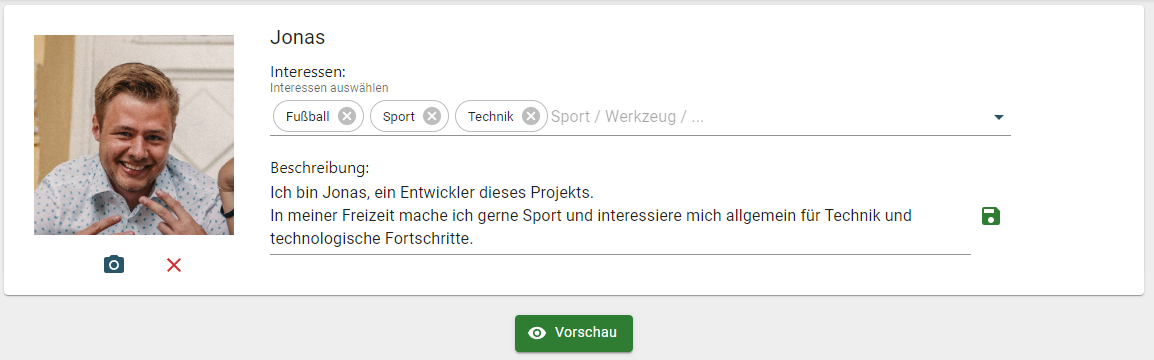
\includegraphics[width=1\textwidth]{figures/implementation/my-profile-header.png}
    \caption{Persönliches Profil}
    \label{fig:myProfileHeader}
  \end{centering}
\end{figure}

\subsection{Blockierte Nutzer}
\label{sec:blockedusers}

Um die Privatsphäre der Nutzer zu schützen, können diese andere Nutzer blockieren.
Blockierte Nutzer können dann nicht mehr auf das Profil des Blockierenden zugreifen und auch keine Nachrichten mehr schreiben.

Über die Profilseite kann ein Nutzer einen anderen Nutzer blockieren.

\begin{figure}[ht!]
  \begin{centering}
    
\includegraphics[width=1\textwidth]{figures/implementation/profile-header.png}
    \caption{Blockieren eines Nutzers}
    \label{fig:blockUser}
  \end{centering}
\end{figure}

Blockierte Nutzer kann man dann in der Anwendung unter dem Menüpunkt \textit{Blockiert} einsehen.
Dort wird jeder Nutzer oder Verein aufgeführt, welcher blockiert ist.
Mit einem Klick auf das „X“ wird der Block aufgehoben.

\begin{figure}[ht!]
  \begin{centering}
    
\includegraphics[width=.5\textwidth]{figures/implementation/blocked.png}
    \caption{Blockierte Nutzer}
    \label{fig:blocked}
  \end{centering}
\end{figure}

\section{Beiträge}
\label{sec:contributions}

Beiträge sind ein anderes wichtiges Feature von „Digital Dahoam“.
Hiermit können Nutzer Informationen austauschen, die für andere Nutzer interessant sein könnten.
Beiträge können von allen Nutzern erstellt werden, die sich registriert haben.
Es gibt folgende Typen von Beiträgen:

\begin{itemize}
  \item \textbf{Anfrage}: Hier können Nutzer eine Anfrage stellen, die dann von anderen Nutzern beantwortet werden kann. Anfragen können auch benutzt werden, wenn bestimmte Gegenstände im Haushalt fehlen, z. B. ein bestimmtes Werkzeug oder ein bestimmtes Lebensmittel.
  \item \textbf{Angebot}: Hier können Nutzer ein Angebot erstellen, das dann von anderen Nutzern angenommen werden kann. Dies kann wie Ebay-Kleinanzeigen benutzt werden, um überflüssige Gegenstände zu verkaufen.
  \item \textbf{Information}: Hier können Nutzer Informationen teilen, die für andere Nutzer interessant sein könnten.
  \item \textbf{Veranstaltung}: Hier können Nutzer Veranstaltungen erstellen, die dann von anderen Nutzern besucht werden können.
\end{itemize}

\subsection{Beiträge erstellen}
\label{sec:createpost}

Beiträge können mit einem Klick auf den Button \textit{Beiträge erstellen} erstellt werden.
Hier öffnet sich ein Pop-up, welchem der Nutzer den Titel, die Beschreibung, den Beitragstyp und die Kategorie des Beitrags eingeben kann.
Außerdem werden für jeden Beitrag das Startdatum, also ab wann der Beitrag gültig ist und angezeigt wird, und das Enddatum, also bis wann der Beitrag gültig ist und angezeigt wird, festgelegt.
Für Veranstaltungen gibt es zusätzlich noch den Ort und das Datum.
Sobald auf \textit{absenden} geklickt wird, wird der Beitrag in der Datenbank gespeichert und auf der Startseite angezeigt.

\begin{figure}[ht!]
  \begin{centering}
    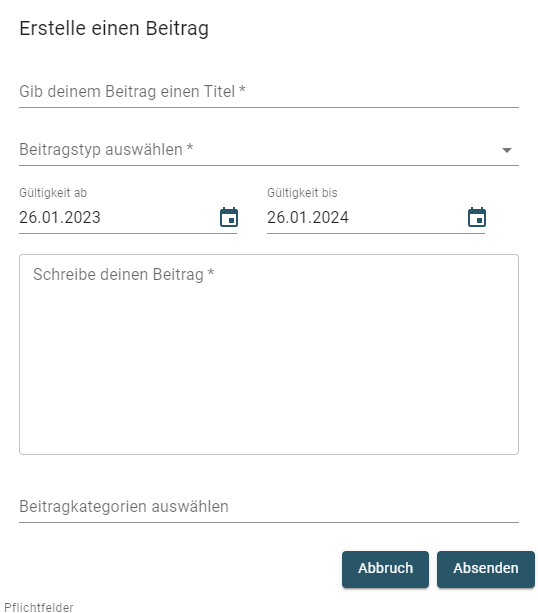
\includegraphics[width=.65\textwidth]{figures/implementation/createpost.png}
    \caption{Beiträge erstellen}
    \label{fig:createpost}
  \end{centering}
\end{figure}


\subsection{Alle Beiträge}
\label{sec:allposts}

Unter \textit{Alle Beiträge} findet man alle Beiträge, die ein valides Gültigkeitsdatum haben. Diese werden mit Titel, Beschreibung, Kategorie und Beitragstyp angezeigt.
Für Veranstaltungen gibt es zusätzlich noch den Ort und das Datum.

\begin{figure}[ht!]
  \begin{centering}
    
\includegraphics[width=.8\textwidth]{figures/implementation/beitrag.png}
    \caption{Beitrag}
    \label{fig:beitrag}
  \end{centering}
\end{figure}

Ein Problem, was es während der Implementierung zu lösen galt, war die richtige Filterung der Beiträge. Die hier verwendete Sortierfunktion (siehe \ref{code:filterPosts}) wurde dann für die restlichen Listen verwendet und die gefilterten Beiträge dort nur noch verfeinert.
Diese musste folgendes erfüllen:

\begin{itemize}
  \item Eigene Beiträge werden immer angezeigt.
  \item Beiträge, die nicht mehr gültig sind, werden nicht angezeigt.
  \item Beiträge von blockierten Nutzern werden nicht angezeigt.
  \item Beiträge müssen nach Datum sortiert werden.
\end{itemize}

Mit dem Klick auf die 3 kleinen Punkte in der rechten oberen Ecke öffnet man das Beitragsmenü. Hier gibt es folgende Punkte:

\begin{itemize}
  \item \textbf{Beitrag zum Merkzettel}: Hinzufügen eines Inhalts zum Merkzettel.
  \item \textbf{Details}: Anzeigen der Details des Beitrags. (siehe \ref{fig:details})
  \item \textbf{Zum Autor}: Direkter Link zum Profil des Autors.
  \item \textbf{Nachricht an Autor}: Direkter Link zur Nachrichtenfunktion, um dem Autor eine Nachricht zu schicken.
\end{itemize}

\begin{figure}[ht!]
  \begin{centering}
    \includegraphics[width=.25\textwidth]{figures/implementation/beitragsmenü.png}
    \caption{Beitragsmenü}
    \label{fig:beitragsmenü}
  \end{centering}
\end{figure}

\clearpage
\subsection{Profilseite}
\label{sec:profilepage}

Auf der Profilseite kann der Nutzer werden seine Beiträge angezeigt.
Hier werden auch abgelaufene Beiträge angezeigt und grau hinterlegt.

\begin{figure}[ht!]
  \begin{centering}
    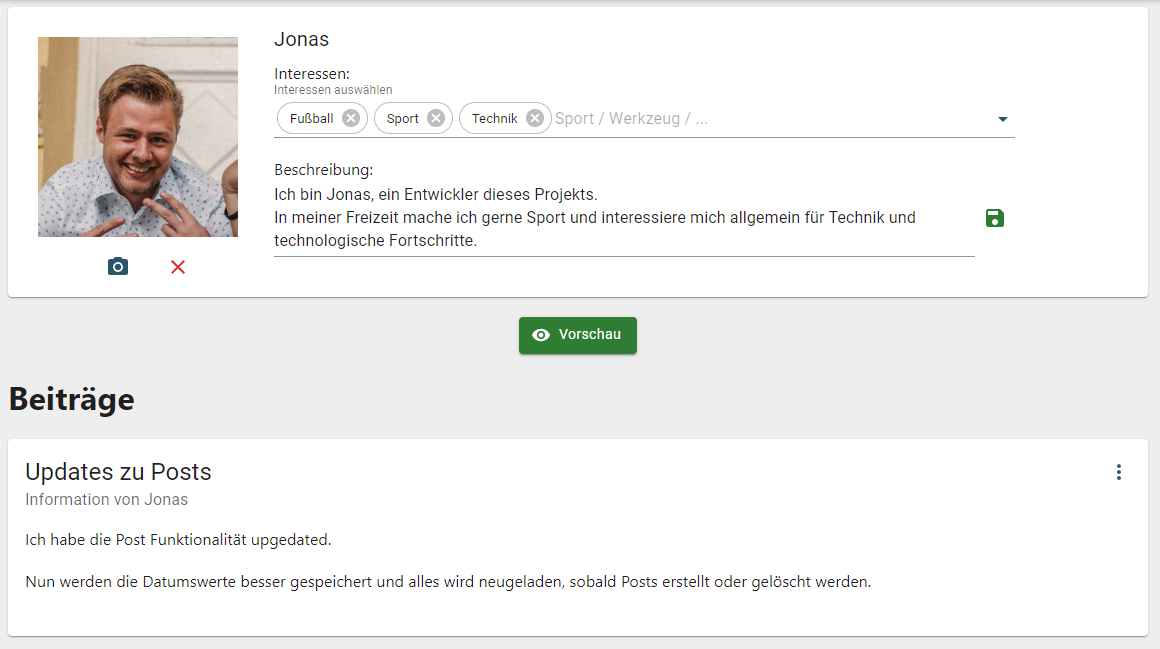
\includegraphics[width=1\textwidth]{figures/implementation/userposts.png}
    \caption{Beiträge des Nutzers}
    \label{fig:userposts}
  \end{centering}
\end{figure}

\subsection{Merkzettel}
\label{sec:bookmark}

Beiträge, die für den Merkzettel markiert sind erscheinen dort, und können dort auch wieder entfernt werden.
Außerdem werden sie nach Beitragstyp gruppiert.

\begin{figure}[ht!]
  \begin{centering}
    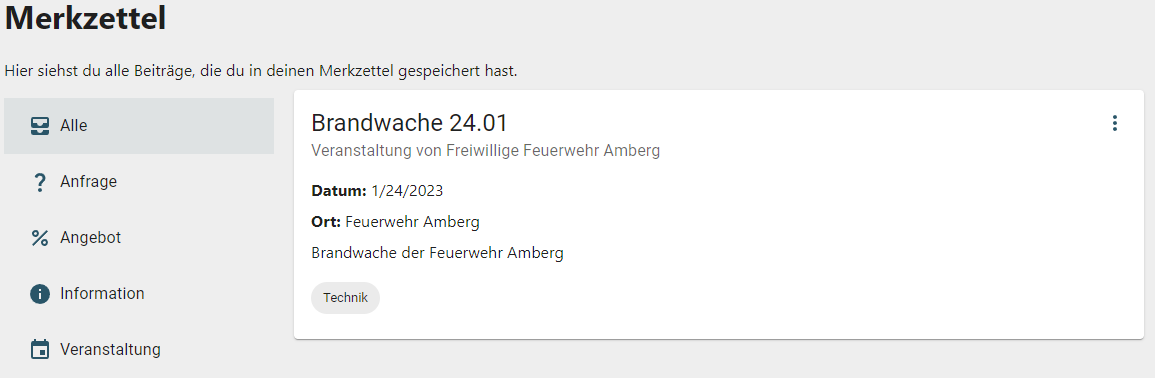
\includegraphics[width=1\textwidth]{figures/implementation/merkzettel.png}
    \caption{Merkzettel}
    \label{fig:merkzettel}
  \end{centering}
\end{figure}

\clearpage
\subsection{Marktplatz}
\label{sec:marketplace}

Auf dem Marktplatz können Personen und Beiträge durchsucht werden.
Durch den Filter auf Kategorien, Informationen oder Veranstaltungen findet man schnell den richtigen Beitrag.

\begin{figure}[ht!]
  \begin{centering}
    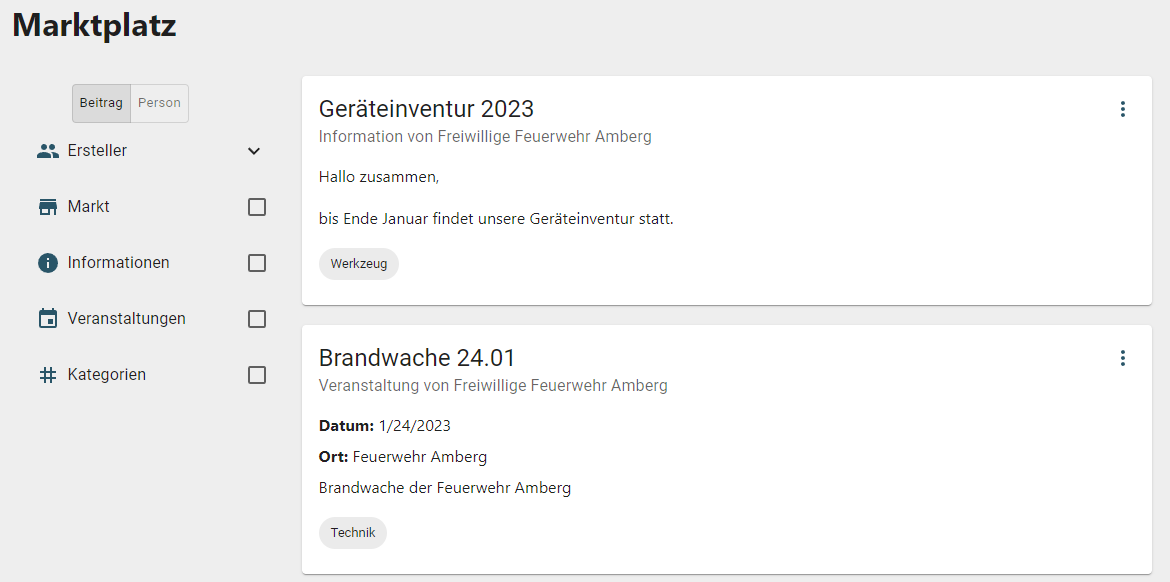
\includegraphics[width=1\textwidth]{figures/implementation/marktplatz.png}
    \caption{Marktplatz}
    \label{fig:marktplatz}
  \end{centering}
\end{figure}


\subsection{Dashboard}
\label{sec:dashboard}

Auf der Startseite werden aktuelle Beiträge aus der Nähe angezeigt, sowie die Veranstaltungen, die der Nutzer auf dem Merkzettel hat.

\begin{figure}[ht!]
  \begin{centering}
    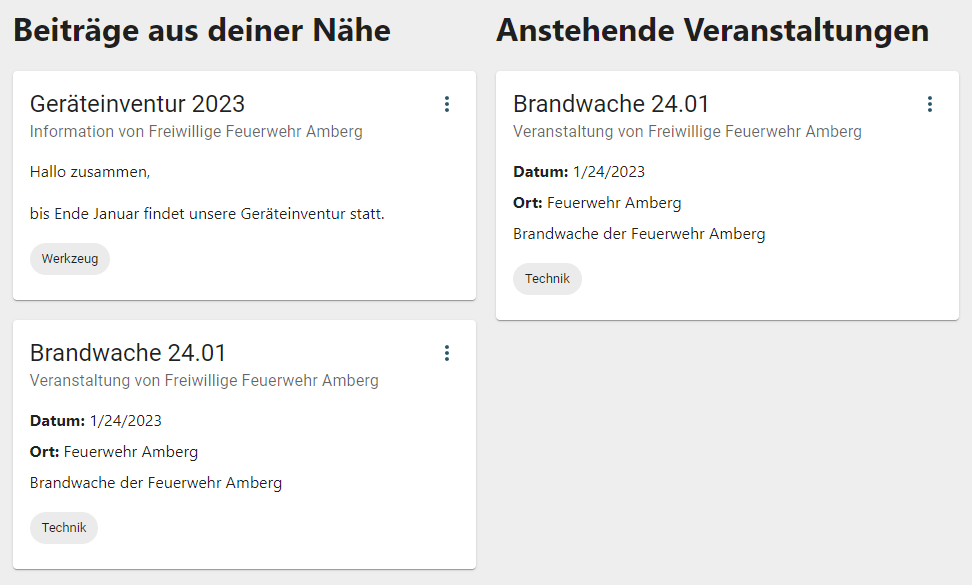
\includegraphics[width=.8\textwidth]{figures/implementation/dashboard.png}
    \caption{Dashboard}
    \label{fig:dashboard}
  \end{centering}
\end{figure}

\section{Chat}
\label{sec:chat}

Ein wichtiges Tool für das soziale Netzwerk \glqq Digital Hometown\grqq \ ist der Chat, da hier die Personen in Kontakt treten und sich austauschen können.

Auf technischer Ebene sind für einen Chat mehrere Technologien erforderlich, wodurch die Umsetzung nicht trivial ist. Neben den Laden der Bereits gesendeten Nachrichten und dem Absenden von Nachrichten, ist es für eine gute Usability notwendig, dass neue Nachrichten sofort bei allen Chatteilnehmern sichtbar sind. Diese Anforderung kann in effizienter Weise durch die Verwendung von bidirektionalen WebSocket-Verbindungen ermöglicht werden.

\subsection{Firebase Realtime Database für den Chat}
\label{sec:firebase_realtime_db_chat}

Für den Chat wird die Firebase Realtime Database (Realtime DB) verwendet. Dadurch wird die Implementierung deutlich vereinfacht, da die entsprechende JavaScript Bibliothek einfach in die React Anwendung integriert werden kann. Eine Echtzeitsynchronisation zwischen den Clients (Browseranwendungen der User) und der Datenbank kann mit geringem Aufwand umgesetzt werden. Die Realtime DB ist eine NoSQL Datenbank.
Die Firebase DB wird in diesem Projekt ausschließlich für den Chat verwendet und hat dabei zwei Hauptwurzelelemente (s. \autoref{fig:hauptwurzel_realtime_db}) verwendet werden. Bei dem Design wurde darauf geachtet, dass die einzelnen Hauptwurzelelemente keine zu große Verschachtelung aufweisen, um eine gute Performanz zu gewährleisten.

\begin{figure}[!htb]
  \centering
  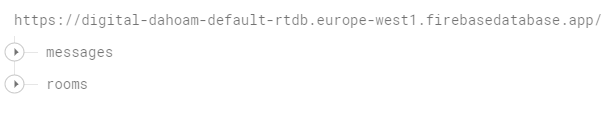
\includegraphics[width=0.8\textwidth]{figures/boas/21_hauptwurzel_realtime_db.png}
  \caption[]{Hauptwurzelelemente der Realtime DB}
  \label{fig:hauptwurzel_realtime_db}
\end{figure}


\subsection{Autorisierung der Nachrichten und Chaträume}
\label{sec:autorisierung_chat}
Eine wichtige Anforderung für die Implementierung einer Chatfunktionalität ist es, dass Nachrichten nur von Mitgliedern des jeweiligen Chatraums gelesen werden können. Dies wird mit den Realtime DB Regeln umgesetzt. Ein Auszug hiervon ist in \autoref{lst:rules_realtime_db} dargestellt. Kurz zusammengefasst ermöglicht diese Konfiguration, dass nur Nachrichten von Benutzern gelesen und geschrieben werden können, die ein Mitglied des Chatraumes sind.

\begin{lstlisting}[language=JavaScript, caption=Realtime DB Regeln für Chatnachrichten, label={lst:rules_realtime_db}]
{
  "rules": {
    "messages": {
      "$roomUid": {
        ".read": "root.child('rooms/' + $roomUid + '/members').hasChild(auth.uid)",
        ".write": "root.child('rooms/' + $roomUid + '/members').hasChild(auth.uid)"
      },
      "messages": {
        ".indexOn": "sendAt"
      }
    },
    ...
  }
}
\end{lstlisting}

\subsection{Benutzung des Chats}
\label{sec:benutzung_chat}

Im folgenden wird anhand von Screenshots die Benutzung des Chats beschrieben. \autoref{fig:chat_screenshot} zeigt die Standardansicht des Chats. Auf der linken Seite sind die Chaträume aufgelistet. Die Chaträume sind in zwei Kategorien unterteilt. Zum einen gibt es die Chaträume, die mit Einzelpersonen erstellt wurden und zum anderen die Chaträume mit mehreren Personen (Gruppenchats). In der Liste der Chaträume werden Gruppenchats mit einem Gruppenicon hervorgehoben.

\begin{figure}[!htb]
  \centering
  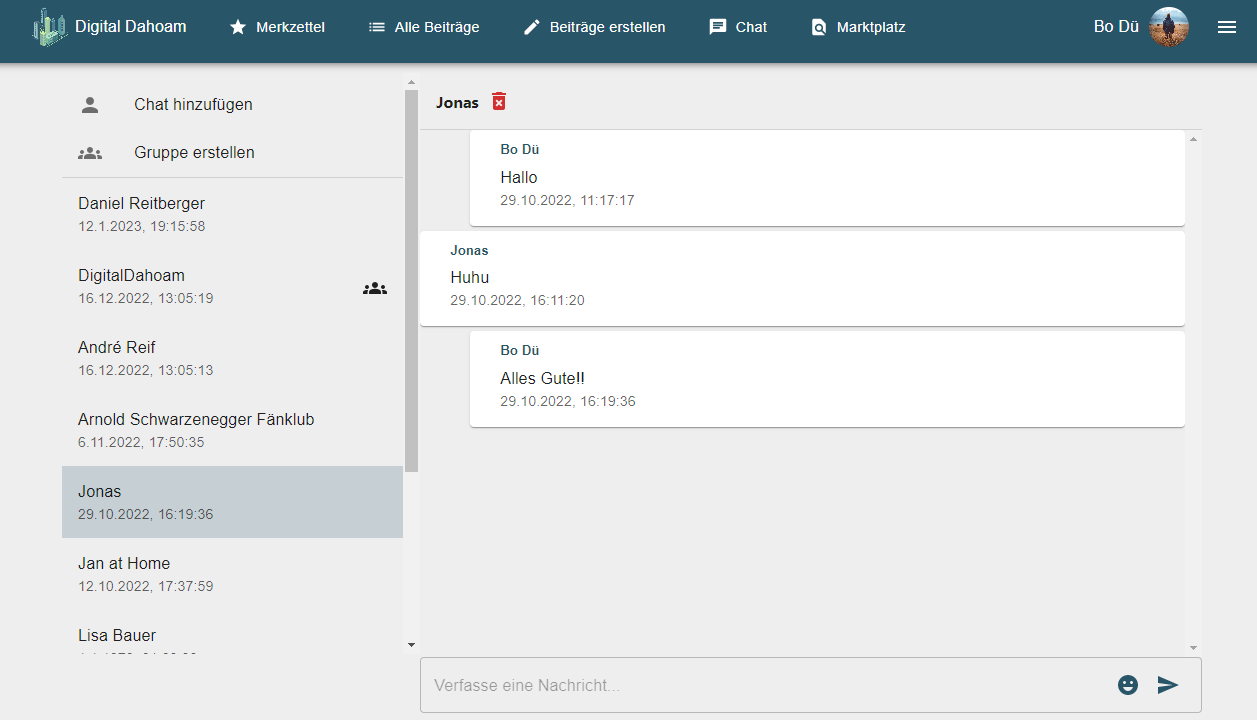
\includegraphics[width=1\textwidth]{figures/boas/21_chat.png}
  \caption[]{Ansicht des Chats in der Anwendung}
  \label{fig:chat_screenshot}
\end{figure}

Über den Button \glqq Chat hinzufügen\grqq \ wir die in \autoref{fig:new_personal_chat} dargestellte Ansicht geöffnet, wo alle Personen der Plattform angezeigt werden. Hier kann ein neuer Chat mit einer Einzelperson erstellt werden.

\begin{figure}[!htb]
  \centering
  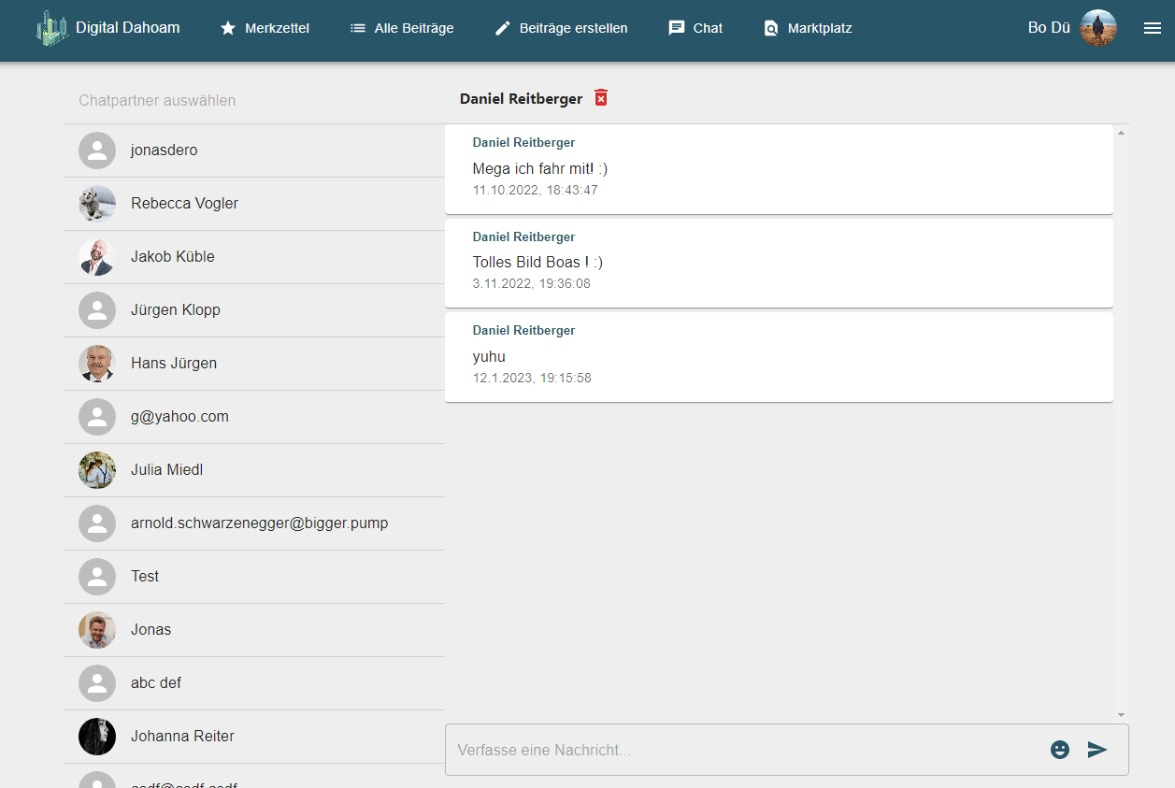
\includegraphics[width=.9\textwidth]{figures/boas/21_new_chat.jpeg}
  \caption[]{Hinzufügen von Chats mit Einzelpersonen}
  \label{fig:new_personal_chat}
\end{figure}

Das Hinzufügen von Gruppenchats erfolgt über den Button \glqq Gruppe hinzufügen\grqq. Der Ablauf sieht hier wie folgt aus. Zuerst wird automatisch ein neuer Chatraum erstellt. Wird dieser ausgewählt, lässt sich über einen Button die in \autoref{fig:edit_chat_group} dargestellte Ansicht öffnen. Hier können die Mitglieder des Chatraumes hinzugefügt werden, indem die entsprechenden Personen aus der Liste ausgewählt werden. Es besteht zudem die Möglichkeit, der Chatgruppe einen anderen Namen zu geben.

\begin{figure}[!htb]
  \centering
  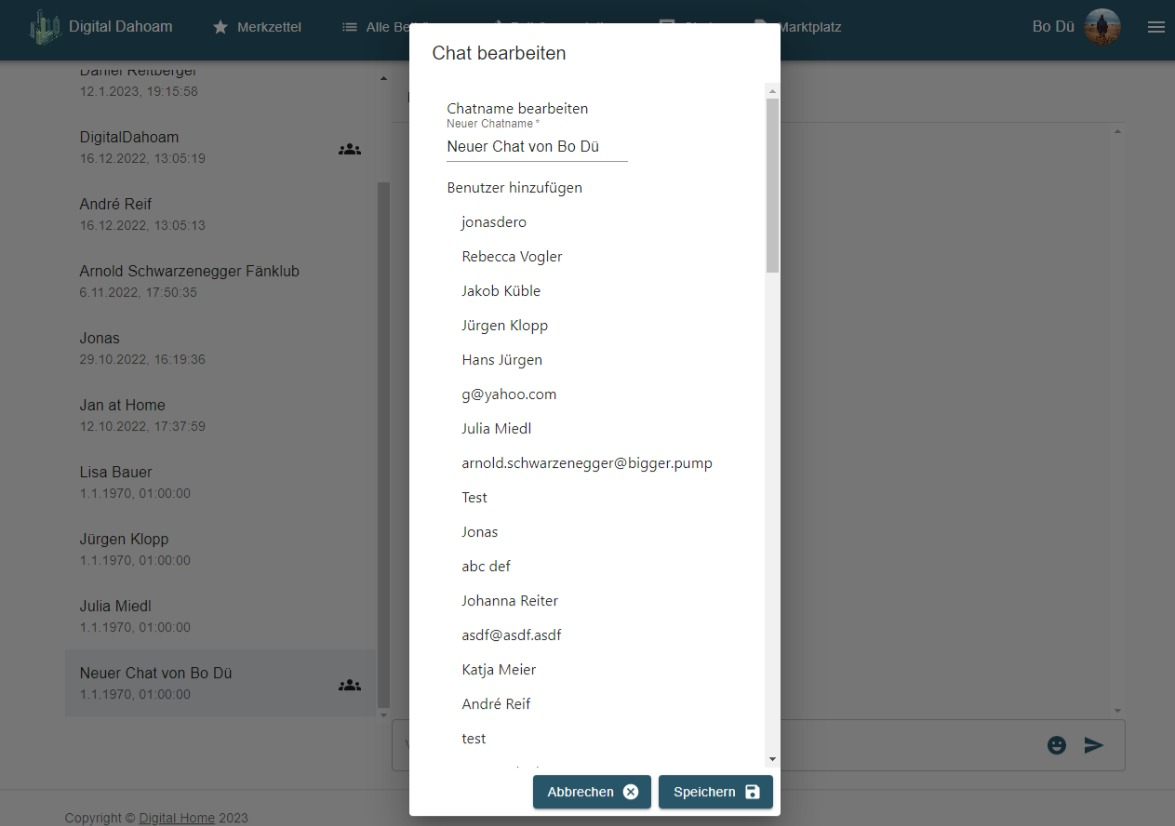
\includegraphics[width=.9\textwidth]{figures/boas/21_edit_chat_group.jpeg}
  \caption[]{Chatgruppe umbenennen und Mitglieder hinzufügen}
  \label{fig:edit_chat_group}
\end{figure}

\subsection{Verknüpfung von Beitragen mit dem Chatraum des Beitragautors}
\label{sec:beitrag_chat_verknüpfung}

Die Motivation des in diesem Absatz beschriebenen Features wird mit folgendem Fallbeispiel erläutert.

Angenommen, ein Benutzer meldet sich an, da er an Fußball interessiert ist und gerne mit Menschen aus seiner Nachbarschaft gerne zum Fußball spielen treffen möchte. Er sieht nun einen Beitrag, der genau diesem Bedürfnis entspricht. Wie in \autoref{fig:beitrag_nachricht} dargestellt, kann er nun über den Button \glqq Nachricht an Autor\grqq direkt zum Chatraum des Beitragautors gelangen. Dort kann er den Beitragautor anschreiben und sich mit ihm zum Fußball spielen treffen.

\begin{figure}[!htb]
  \centering
  \includegraphics[width=.7\textwidth]{figures/boas/21_beitrag_nachricht.jpg}
  \caption[]{Möglichkeit von einem Beitrag direkt zum Chatraum des Beitragautors zu gelangen}
  \label{fig:beitrag_nachricht}
\end{figure}

Im Hintergrund muss dafür der gemeinsame Chatraum ermittelt werden. Falls dieser noch nicht existiert, muss er erstellt werden. Wird dann der Nutzer auf die Chatseite weitergeleitet, öffnet sich automatisch der entsprechende Chatraum.

\chapter{Testing}
\label{ch:testing}

Diese Kapitel beschäftigt sich mit dem Prozess des Testens in diesem Projekt. Dabei soll zunächst wird etwas Theorie vorgestellt, in der klar gemacht werden soll, was Testen eigentlich ist, wie der Test Prozess im Projekt nach SCRUM gelebt wurde und welche Aufgaben dem Tester zufallen. Abgeschlossen wird dieses Kapitel dem beispielhaften Aufzeigen der Umsetzung der definierten Testmethoden in diesem Projekt.

\section{Definition Testen}
\label{sec:DefTest}

Softwaresysteme sind ein wesentlicher Bestandteil des Lebens: von Fachanwendungen (z.B. im Bankwesen) bis hin zu Verbraucherprodukten (z.B. Autos). Die meisten Menschen haben bereits Erfahrungen mit Software gemacht, die nicht wie erwartet funktioniert hat. Software, die nicht korrekt arbeitet, kann zu vielfältigen Problemen führen, u.a. zu Geld-, Zeit- oder Imageverlust, sogar bis hin zu Verletzungen oder Tod.
Softwaretesten ist ein Mittel, die Qualität von Software zu beurteilen und das Risiko einer Fehlerwirkung im Betrieb zu reduzieren.
Es ist eine gängige Fehleinschätzung, dass Testen ausschließlich darin besteht, Tests auszuführen, d.h. im Sinne von: die Software auszuführen und die Ergebnisse zu prüfen. Softwaretesten ist ein Prozess, der viele unterschiedliche Aktivitäten umfasst. Testen beinhaltet also auch die Prüfung von Arbeitsergebnissen wie Anforderungen, User-Stories und Quellcode im Rahmen von Reviews. Eine weitere gängige Fehleinschätzung ist, dass sich Testen ausschließlich auf die Verifizierung von Anforderungen, User-Stories oder anderen Spezifikationen konzentriert. Auch wenn das Testen es erfordert, zu prüfen, ob das System spezifische Anforderungen erfüllt, so umfasst es auch die Validierung, also die Prüfung, ob das System in seiner Einsatzumgebung die Bedürfnisse von Benutzern und anderen Stakeholdern erfüllen wird.

\section{Aufgabengebiet als Tester}
\label{sec:AufgTest}

Das Testen ist untrennbar mit der Entwicklung verwoben. Teammitglieder mit Testfokus decken mehrere Rollen ab: zum einen, die des Testers (operative Aufgaben), zum anderen die des Testmanagers (Strategische Aufgaben) und schließlich auch die des Qualitätsmanagers.

Jedes agile Team besteht aus zumindest ein bis zwei ausgebildete Tester. Weiterhin stehen dem Team ergänzend noch einige Support-Teams oder auch einzelne Fachexperten zur Verfügung, die für Spezialthemen herangezogen werden können (s. \autoref{fig:AufgGebietTester}).

\begin{figure}[!htb]
  \centering
  \includegraphics[width=.9\textwidth]{figures/rebecca/Aufgaben_Tester.png}
  \caption[]{Aufgabengebiete des Testers}
  \label{fig:AufgGebietTester}
\end{figure}

Vereinfacht kann die Teamzusammenstellung wie folgt dargestellt werden (\autoref{fig:team_position_tester}).

\begin{figure}[!htb]
  \centering
  \includegraphics[width=.9\textwidth]{figures/rebecca/Position_Tester.png}
  \caption[]{Teamzusammenstellung und Position der Tester}
  \label{fig:team_position_tester}
\end{figure}

\section{Testen im agilen Projekt}
\label{sec:testen_agil}

Das Testen hat auch in SCRUM einen hohen Stellenwert. Die Rolle des Testers sollte ein fester Bestandteil eines cross-funktionalen Teams, die Qualitätssicherung automatisch in jedem Entwicklungszyklus integriert sein. Das agile Testen im SCRUM muss so gestaltet sein, dass es die Ziele der agilen Entwicklung unterstützt. Das heißt, es muss auf hohe Kundenzufriedenheit, hohe Produktivität und hohe Entwicklungsgeschwindigkeit ausgerichtet sein. Es muss schnell auf Änderungen reagieren können und selbstorganisiert sein.
Als agiles Testen wird das Testen von Software im Rahmen eines agilen Entwicklungsprojekts bezeichnet. Testen in agilen Entwicklungsprojekten bedarf dabei vor allem eines Fokus auf die Unterstützung des Entwicklungsteams.


\subsection{Wann in Scrum Testen}
\label{sub:WannTestenScrum}

Es gilt der Grundsatz von Realisierung und Test non-stop. Während des Sprints muss dafür gesorgt werden, dass die „Tester“ vom ersten Tag an ins Team integriert sind und parallel mit (bzw. zusammen mit) den „Entwicklern“ an der Realisierung der Stories arbeiten. Schlüsselfertigkeiten hierfür sind:

\begin{itemize}
  \item Die Beteiligung der Tester an der Sprint-Planung und den Weekly Scrum Meetings
  \item Die zeitliche Verschränkung von Entwicklungs- und Testaktivitäten. Hierzu sind Prinzipien wie „Test Driven Development“ bzw. „Test First“ und Pairing zwischen Entwicklern und Testern geeignet
  \item Die Kombination von systematischen Tests und explorativen Tests. Letztere liefern besonders schnell Feedback und finden Fehler, die von systematischen Tests ggf. nicht gefunden werden können. Diese wurden von mir als Tester durchgeführt.
  \item Die transparente Repräsentation von Tests in der Planung und Statusverfolgung durch geeignete Darstellung auf dem Taskboard, dem zentralen Planungsmittel des agilen Teams
\end{itemize}

\begin{figure}[!htb]
  \centering
  \includegraphics[width=.9\textwidth]{figures/rebecca/Wann_In_Scrum_Testen.png}
  \caption[]{Wann in Scrum Testen}
  \label{fig:WannTesten}
\end{figure}

\section{Test-Prozess}
\label{sec:TestProzess}

Der fundamentale Testprozess (FTP) ist einer der am verbreitetsten Testprozesse und mittlerweile internationaler ISTQB-Standard. Der Prozess beinhaltet verschiedene Testaktivitäten, welche während des gesamten Testprozesses abgedeckt sein sollten. Diese Aktivitäten sind die Testplanung, der Testentwurf, die anschließende Testimplementierung sowie deren Ausführung, eine anschließende Testauswertung sowie ein abschließender Testabschluss. Jeder der im Folgenden erklärten Testtypen (Entwicklertest, Inkrement Test und Release-Test) soll all diese Testaktivitäten strukturiert in unterschiedlicher Intensität anwenden. Die Testplanung findet während des Sprint-Plannings und des Daily Scrums (weekly), der Testentwurf, die Testimplementierung und -ausführung während des Sprints, die Testauswertung während des Sprint-Reviews sowie der Testabschluss während der Sprint-Retrospektive stattfinden sollen. Für die einzelnen Testaktivitäten in den jeweiligen Testtypen sollten die folgenden Aspekte genutzt werden: eine Testbasis, gegen welche getestet wird (z.B. Anforderungen im Backlog), die Testobjekte, welche getestet werden (z. B. ein Inkrement), die Teststufen und Testarten, welche durchgeführt werden (z. B. Systemtest als Teststufe und Regressionstest als Testart) sowie die verschiedenen Testwerkzeuge, welche das Testen unterstützen. (s. \autoref{fig:TestProzessBild})

\begin{figure}[!htb]
  \centering
  \includegraphics[width=.9\textwidth]{figures/rebecca/Testprozess.png}
  \caption[]{Testprozess}
  \label{fig:TestProzessBild}
\end{figure}

\subsection{Entwicklertest}
\label{sub:EntwicklerTest}

Der Entwicklertest findet während der täglichen (in diesem Projekt wöchentlichen) Entwicklungsarbeit statt. Das Test Ziel ist die Validierung der täglichen (wöchentlichen) Entwicklungsergebnisse gegen die Sprint-Tasks. Jeder Entwickler kümmert sich um seine aktuellen Sprint-Tasks, welche hier als Testbasis dienen, aus der die Testfälle abgeleitet werden müssen. Das Daily Scrum findet wie üblich, es werden allerdings zusätzlich auch die Testaufgaben und Testfälle besprochen. Diese Tests (s. \autoref{fig:EntwicklerTest}) werden vom Entwickler übernommen.

\begin{figure}[!htb]
  \centering
  \includegraphics[width=.9\textwidth]{figures/rebecca/Entwickler_Test.png}
  \caption[]{Entwickler-Test}
  \label{fig:EntwicklerTest}
\end{figure}

\subsection{InkrementTest}
\label{sub:InkremenTest}

Der Entwicklertest findet im täglichen Rahmen statt, wohingegen der Inkrement-Test erst gegen Ende eines Sprints durchgeführt, wenn das Inkrement fertig wird. Obwohl Aktivitäten im Entwicklertest eine kontinuierliche Qualitätsüberwachung des Inkrements ermöglichen, ist am Ende eines Sprints ein dedizierter Inkrement-Test notwendig, um folgende Testziele zu gewährleisten.

\begin{itemize}
  \item Die korrekte Funktionsweise des im Sprint entwickelten Inkrements und des korrekten Zusammenspiels mit früher entwickelten Inkrementen soll gezeigt werden.
  \item Es soll sichergestellt werden, dass frühere Inkremente nicht verändert wurden. Der Test kann je nach Sprintlänge nach einer Woche oder auch erst nach vier Wochen durchgeführt 
\end{itemize}

Gegen Ende des Sprints ist ein Regressionstest sehr wichtig ist, damit die alte Funktionalität immer noch richtig läuft, nachdem neue Funktionalität hinzugefügt wurde.
Die Testbasis sind im Gegensatz zum Entwicklertest nicht nur die einzelnen Sprint-Tasks, sondern das gesamte Sprint-Backlog, welches das zu liefernde Inkrement, hier auch das Testobjekt, definiert. Die Definition of Done besagt, wann ein Task wirklich fertig ist, wozu u. a. auch das Testen gehört. Im abschließenden Review Meeting, wird diese „Definition of Done“ vom Team zusammen mit dem Product Owner ausgewertet, ob sie für die Entwicklung und das Testen des Inkrements erfüllt wurde. Zur Testdurchführung gehören im Inkrement-Test als Teststufen neben dem Entwicklertest insbesondere auch der Systemtest, der prüft, ob das entsprechende Inkrement als ein Ganzes funktioniert und so vom Benutzer akzeptiert wird. Als Testarten gehören zu diesem Test-Typ nicht nur die funktionalen Tests und Regressionstests, sondern insbesondere auch die nicht-funktionalen Tests, wie beispielsweise Performanz Tests, Usability-Tests usw.

\begin{figure}[!htb]
  \centering
  \includegraphics[width=.9\textwidth]{figures/rebecca/Inkrement_Test.png}
  \caption[]{Inkrement-Test}
  \label{fig:InkrementTest}
\end{figure}

\subsection{Release-Test}
\label{sub:release_test}

Der Release-Test wird das Produkt in seiner Gesamtheit getestet. Der Release-Test findet abschließend nach den Inkrementtests in Form eines dedizierten Sprints statt. Häufig wird eine Software inpotenziell fertigen Inkrementen entwickelt, welche aber anschließend zu einem gesamten Release zusammengefasst wird. Am Anfang wird geplant, nach wie vielen Sprints ein Release üblicherweise fertig sein soll. Der Release-Test kann nun ebenfalls als ein Sprint aufgebaut werden und ist damit weiter Scrum-Konform. Die Testbasis ist hier nun das gesamte Product Backlog, da hier nicht nur ein Inkrement nach einem Sprint, sondern das gesamte Produkt das Testobjekt ist. Anstatt eines Sprint-Backlogs kann analog ein sogenanntes Test-Backlog erstellt werden, welches die gesamten Release-Tests enthält. Als Teststufen enthalten diese Release-Tests Systemintegrationstests, Inbetriebnahmetests und insbesondere Akzeptanztests. Im Release-Test können die Testfälle aus den Inkrementtests wiederverwendet werden, sodass für den Testentwurf kein erheblicher Zusatzaufwand entsteht. Als Testart ist hier neben den funktionalen und nicht-funktionalen Tests auch das sogenannte End-To-End-Testing zu finden, welches über das gesamte System und Produkt im Zusammenspiel aller Komponenten stattfindet. Für die Durchführung der Tests wird das Test-Backlog analog zum Sprint-Backlog in Test-Tasks aufgeteilt, welche täglich entwickelt und durchgeführt werden. Weiterhin findet ein Daily Scrum statt um die Arbeit zu besprechen. Auf stündlicher Basis findet neben den Tests auch das Debugging statt, um Fehler zu finden und zu beheben. Am Ende des Tages steht ein Test-Report an. Am Ende des Sprints findet nicht nur eine Auswertung der speziellen Definition of Done bezüglich des Releases statt, sondern ebenfalls die finale Kundenabnahme des Produktes.

\begin{figure}[!htb]
  \centering
  \includegraphics[width=.9\textwidth]{figures/rebecca/Release_Test.png}
  \caption[]{Release-Test}
  \label{fig:ReleaseTest}
\end{figure}

\section{Umsetzung im Projekt}
\label{sec:UmsetzungTest}

Hier soll nun genauer erläutert werden, welche der Testmethoden in dem Projekt genutzt wurden, um möglichste hohe fehlerfrei Qualität unsere Plattform zu gewährleisten.

\subsection{Testen gegen User-Stories}
\label{sub:UmsetzungTestGGUserStories}

Beim Abtesten der User-Stories wurde das Verfahren des Black-Box Testens angewandt. Bei einem Black-Box-Test werden die Testfälle ausschließlich aus der Spezifikation (User-Stories) des zu testenden Objekts abgeleitet, ohne dabei dessen innere Struktur, also Architektur und Code, zu berücksichtigen (- diese werden als „Black Box“ behandelt). Es wird also nur das von außen sichtbare Verhalten des Testobjektes beobachtet.

\begin{figure}[!htb]
  \centering
  \includegraphics[width=.9\textwidth]{figures/rebecca/Black_Box_Testing.jpg}
  \caption[]{Black-Box-Testing}
  \label{fig:BlackBoxTest}
\end{figure}

Dabei wurde als Akzeptanzkriterium die Defintion of Done der einzelnen User Stories genutzt. Dabei wurde der Fokus auf das positive Testing und negative Testing gelegt. Zusätzlich wurden aber auch einige Grenzwert-Testfälle spezifiziert, wo dies nötig war, und durchgeführt.

\textbf{Positive Testing:} \\
Positivtests sind eine Art von Softwaretests, bei denen davon ausgegangen wird, dass alles so abläuft wie erwartet. Es wird mit der Annahme durchgeführt, dass nur gültige und relevante Dinge auftreten werden.

\textbf{Negative Testing:} \\
Negativtests sind eine Art von Softwaretests, die durchgeführt werden, um das System auf unerwartete Bedingungen zu prüfen. Negative Tests spielen eine wichtige Rolle bei der Entwicklung leistungsfähiger Software. Dabei wird geprüft, wie sich die Software unter solchen unerwarteten Bedingungen verhält.

\begin{figure}[!htb]
  \centering
  \includegraphics[width=.9\textwidth]{figures/rebecca/Neg_Pos_Testing.png}
  \caption[]{Negative vs. Positive Testing}
  \label{fig:negativ_vs_positiv_testing}
\end{figure}

\textbf{Grenzwert-Testing:} \\
Das Testen von Grenzwerten testet extreme Grenzen der Eingangswerte. Unter extreme Grenzen fal-len Enden wie Start-End-, Lower-Upper-, Maximum-Minimum-, Just Inside-Just Outside-Werte. Das Testen wird als 'Testen von Grenzwerten' bezeichnet.
Die Umsetzung soll nun im Folgenden anhand eines Beispiels genauer erklärt werden. In diesem Beispiel wird der Fokus nur auf die Angabe des Gültigkeitsdatums gelegt (DH-179).

\begin{figure}[!htb]
  \centering
  \includegraphics[width=.9\textwidth]{figures/rebecca/Beispiel_User_Story_Test.png}
  \caption[]{Beispiel User-Story für Test}
  \label{fig:BespielUserStory}
\end{figure}

\begin{figure}[!htb]
  \centering
  \includegraphics[width=.9\textwidth]{figures/rebecca/Umsetzung_Testfaelle}
  \caption[]{Umsetzung der Testfaelle}
  \label{fig:UmsetzungTestFaelle}
\end{figure}

\subsection{Regressions-Test}
\label{sub:UmsetzungTestRegression}

Wenn eine Software durch die Einführung neuer oder geänderter Funktionen an Funktionalität verliert, spricht man von einem Rückschritt zu einem weniger entwickelten Zustand. Selbst geringfügige Änderungen an der Software oder am ursprünglichen Code können zu erheblichen Fehlern wie Abstürzen, Störungen und teilweisem oder vollständigem Verlust der Funktionalität führen.
Regressionstests dienen dazu, diese Fehler zu erkennen und die Anwendung wieder zu stabilisieren. Sowohl funktionale als auch nicht-funktionale Testverfahren bewerten die Auswirkungen neuer Funktionen auf den bestehenden Code.
In diesem Projekt wurde das folgendermaßen gelebt: Die Testfälle gegen User-Stories (4.5.1) wurden priorisiert. Anschließend wurden 1-2 Testfälle ausgewählt zu jeder User-Story, welche nach einer Optimierung oder Änderung des dazugehörigen Feature jedes Mal mit ausgeführten wurden. Das bedeutet zum Beispiel, dass zunächst die Funktion des Beitrags erstellen möglich war. Anschließend wurde die Funktion des Gültigkeitsdatums hinzugefügt. Danach wurde überprüft, dass alle vorherigen Funktionen weiterhin die Defintion of Done erfüllen und alles weiterhin fehlerfrei funktioniert.
Eine vollständige Wiederholung aller Testfälle wurde im letzten Sprint vor dem Release vorgenommen (Release Test), um sicherzustellen, dass bei der Übergabe zum Kunden alles fehlerfrei funktioniert.

\begin{figure}[!htb]
  \centering
  \includegraphics[width=.9\textwidth]{figures/rebecca/Regressions_Test.png}
  \caption[]{Regressions-Test}
  \label{fig:Regressionstest}
\end{figure}

\subsection{Feld-Test}
\label{sub:UmsetzungTestFeld}

Ein Feldtest ist die Erprobung einer produktionsfähigen Vorabversion einer Software durch eine repräsentative Anzahl an von Anwendern. Das Ziel eines Feldtests ist das Erkennen von noch nicht komplett spezifizierten Einsatzumgebungen und Bedingungen sowie dem Prüfen auf Akzeptanz des Marktes.
Dazu wurde eine bereite Anzahl an potentiellem Nutzer ins Visier genommen. Da die Plattform Generationenübergreifend sein soll, wurden daher Testpersonen mit unterschiedlichem Alter, unterschiedlichem Background Wissen und unterschiedlichen Interessen ausgewählt.
Für die Durchführung des Feld-Testes wurde eine Guideline erstellt und der Tester hat sich zusammen mit der Testperson an einen Rechner gesetzt und die aktuelle Plattform ausprobiert. Der Tester hat dabei die Testperson nur gebeten gewisse Aktionen durchzuführen und hat die Testperson gebeten, dabei unentwegt Rückmeldung darüber zu geben, welche Gefühle er dabei empfindet und wie ihm die bestehenden Features gefallen. Abgeschlossen wurde der Test dadurch, dass die Personen ein kurzes Feedback geben sollten.
Der Test wurde insgesamt drei Mal durchgeführt mit jeweils 6 Personen, und das Ergebnis wurde anschließend im Team besprochen, wo etwaige Änderungen vorgenommen werden müssen beziehungsweise welche Features eventuell neu priorisiert werden müssen.

\begin{figure}[!htb]
  \centering
  \includegraphics[width=.9\textwidth]{figures/rebecca/Feld_Test_Konzept.png}
  \caption[]{Feld-Test}
  \label{fig:Feldtest}
\end{figure}

Teilnehmer:
\begin{itemize}
    \item P. Vogler (Alter: 53, weiblich, Bankkauffrau)
    \item N. Vogler (Alter: 55, männlich, Berufsschulehrer)
    \item D. Bandac (Alter: 26, männlich, Requirements-Ingenieur)
    \item D. Blana (Alter: 27, weiblich, Zahntechnikerin)
    \item T. Scholl (Alter: 36, männlich, System-Tester)
    \item K. Warmuth (Alter: 42, weiblich, Büro-Angestellte)
  \end{itemize}

\subsection{Exploratives-Testen}
\label{sub:UmsetzungTestExplorativ}

Bei dieser Methode stehen nicht Testpläne im Mittelpunkt, sondern die Tester „entdecken“ die Anwendung schrittweise selbst, indem sie diese benutzen. Parallel dazu erstellen die ersten Testfälle und optimieren sie iterativ in dem Maße, in dem mehr über die Anwendung gelernt wird. Gefragt sind hierbei vor allen Dingen Intelligenz, Intuition und Erfahrung. Im Gegensatz zu den klassischen Testmethoden – die dadurch keineswegs obsolet werden – fokussiert sich der explorative Ansatz auf die grundsätzliche Benutzbarkeit der Anwendung. Denn Schwächen in der Darstellung, umständliche Arbeitsabläufe oder logische Brüche, werden oft erst im Nutzererlebnis offenbar.

\begin{figure}[!htb]
  \centering
  \includegraphics[width=.9\textwidth]{figures/rebecca/Exploratives_Testen.png}
  \caption[]{Exploratives Testen}
  \label{fig:explorativesTesten}
\end{figure}

Hierbei spezialisierte vor allem Ende des jeden Sprints fokussiert. Dabei wurde überprüft, welche neuen Funktionen implementiert wurden. Anschließend wurden diese in den Fokus genommen und mit den bisherigen Funktionen zusammen ausprobiert. Dabei werden auch bereits bestehende Testfälle optimiert und neue Testfälle hinzugefügt (s. Dazu 4.5.1). Hinzu kommt, dass dabei auch die Usability der einzelnen Funktionen überprüft wurden um die Qualität unserer Plattform aus der Sicht des Endbenutzers zu bewerten.
Bei Auffälligkeiten wurden im Weekly Meeting Rücksprache mit dem Team gehalten, um etwaige Änderungen am Design zu erörtern und in die Wireframes wenn nötig einzubinden.
Bei Fehlern wurde ein Fehlerbericht erstellt (Bug-Bericht), und dem jeweiligen Entwickler in Jira zugewiesen.
\chapter{Fazit}
\label{ch:conclusion}

Abschließend lässt sich zum erreichten Ergebnis festhalten, dass wir eine Plattform geschaffen haben, die dem gesetzten Projektziel entspricht. Die Plattform bietet mit ihren einzelnen Features die Möglichkeit der Vernetzung von Nachbarn. Hierbei sind vor allem die generalistisch zu verwendenden Beiträge zu nennen. Mit den Beiträgen erreichen Menschen oder Vereine die nötige Reichweite, um wichtige Informationen preiszugeben. Des weiteren ist es durch die Möglichkeit etwas anzubieten (Geben) bzw. Anfragen zu stellen (Nehmen) möglich, das Menschen in der Nachbarschaft in Kontakt kommen bzw. sich über die Plattform kennenlernen können.

Die Benutzbarkeit der Plattform ist durch die intuitive und übersichtliche Benutzeroberfläche gegeben. Die Benutzeroberfläche ist hierbei in erster Linie für Desktop-Geräte optimiert, kann jedoch aufgrund der ausgewählten Technologie mit begrenztem Aufwand für mobile Geräte angepasst werden.

Durch die Verwendung von Firebase, das von Google betrieben wird, sowie von Vercel zum Hosting der Plattform, ist eine sehr hohe Verfügbarkeit der Plattform gegeben.

Auch wenn es Mangels der Zeit nicht möglich war, alle Features in einer optimalen Qualität zu implementieren, haben wir es in der knappen Zeit geschafft, eine funktionierende Plattform zu entwickeln, die in iterativen Schritten immer weitere Features dazugewonnen hat. Die Aufgabenstellung an sich hätte sicherlich eine Vielzahl weiterer Features ergeben, umso wichtiger war unsere Diskussion, welche Features für die Plattform im ersten Schritt wirklich notwendig sind. Ich finde, unsere Plattform entspricht diesem Prinzip und kann sich deshalb sehen lassen.

\appendix
\pagenumbering{Alph}
\renewcommand{\thechapter}{\Alph{chapter}}
\renewcommand{\thesection}{\Roman{section}}
\renewcommand{\thesubsection}{\Roman{subsection}}
\renewcommand\floatpagefraction{0.1}
\clearpage
\chapter{Anhang}
\label{appendix:annex}

\section{Bilder}
\label{annex:images}

\begin{figure}[ht!]
  \begin{centering}
    \includegraphics[width=1\textwidth]{figures/implementation/firestore-user.png}
    \caption{Benutzerdatensatz in Firestore}
    \label{fig:firestoreUser}
  \end{centering}
\end{figure}

\begin{figure}[ht!]
  \begin{centering}
    \includegraphics[width=.75\textwidth]{figures/implementation/details.png}
    \caption{Beitragsdetails}
    \label{fig:details}
  \end{centering}
\end{figure}

\clearpage
\section{Code}
\label{annex:code}

\begin{lstlisting}[language=JavaScript, label=code:filterPosts, title={Filterfunktion der Beiträge}]
const filtered = posts
.filter((post) => !currentUser?.blocked?.includes(post.author.id))
.filter((post) => {
  // check validity
  if (currentUser?.id === post.author.id) {
    return true
  }

  if (!(post.validityStart && post.validityEnd)) {
    // no validity set
    return true
  }
  console.log(
    moment(post.validityStart).toDate().getTime(),
    moment(post.validityStart).toDate().getTime() <= new Date().getTime(),
  )
  if (
    moment(post.validityStart).toDate().getTime() >= new Date().getTime() &&
    moment(post.validityEnd).toDate().getTime() <= new Date().getTime()
  ) {
    return true
  } else {
    return false
  }
})
\end{lstlisting}

\backmatter
\listoffigures
\listoftables
\bibliographystyle{IEEEtran}
\bibliography{refs}

\end{document}
